\chapter{Microbial population structure and genetic heterogeneity in a hypersaline environment}

\section{Abstract}

\section{Introduction}

The increasing number of microbial genomes sequenced over the last years, driven by the higher-throughput and lower cost of sequencing technologies, has pushed the field of comparative genomics, allowing for comparisons of the genomes of organisms from the same genus and even closely related strains \cite{Fricke:2011gy,Doroghazi:2013gf,Grad:2013tc,Reno:2009bq}, in search of insights into their evolutionary history and environmental adaptation \cite{Reno:2009bq,ZhuofeiXu:2011fp}. This has been a particularly powerful approach in medical microbiology, where multiple cultivated strains are available, allowing for a deep coverage of microbial species of medical interest \cite{Feero:2011fr}. Some of this has been replicated in microorganisms isolated from the environment (non-clinical settings), including members of the \textit{Vibrio} genus \cite{Cordero:2012ik} and \textit{Sulfolobus} \cite{Reno:2009bq}.
 
The development of culture-independent approaches, has allowed to remove some of the restrictions of culture-based comparative genomics, by allowing us to capture directly the taxonomic, functional and genetic diversity of the members of microbial community, by direct sequencing of their DNA \cite{Bragg:2014kv}. The main challenge in metagenomic studies, is given by the complexity of some microbial communities, allowing only to capture a glimpse of the taxonomical and functional diversity, and not providing enough information to explore the genetic diversity that is present. 

In the case of low to moderate microbial communities (~2-30 dominant microbial species), using the appropriate sequencing technologies and sampling approaches, it is possible to reconstruct the genomes for some of the dominant members of the community \cite{Bragg:2014kv}. But in reality, these genomes do not represent a single clone, but are a composite of multiple related strains \cite{Podell:2013kx,Allen:2005dg}, where this fine-scale genetic variation could have functional relevance for the members of the community \cite{Lo:2007ht,Hemme:2010ds,Palenik:2009kx}.

Several studies have approached the study of microbial communities with the goal of quantifying the level of fine-scale genetic variation present in its members \cite{Wilmes:2009bn}, by using metagenomic approaches. These studies can be divided in two groups, based on the type of reference used to quantify genetic heterogeneity. A first group, approached a natural microbial community, obtained metagenomic sequence from the system, and then used reference genomes from isolates to quantify the genetic variation present in the microbial community. Examples of this approach include the study of \textit{Synechococcus} coastal populations \cite{Tai:2011jo} and in the human gut microbiome \cite{Schloissnig:2012hx}. The limitation of this type of studies, is that not necessarily the reference genomes used are derived from the same environment as the metagenomic sample. In addition, it is possible to miss novel and abundant groups, by just focusing on the genomes that are available through isolates \cite{Podell:2013kx,Herlemann:uy}. A second type of approach, is to use assembly-based metagenomics, which allows to recover a set of habitat-specific genomes, on which the genetic heterogeneity present in the community can be quantified. Although this approach provides a more complete and less biased picture of the genetic diversity, it is limited to communities with low species diversity, such as acid mine drainage \cite{Allen:2007ju} or heavy-metal contaminated sites \cite{Hemme:2010ds}.

The metagenomic studies carried out on the Lake Tyrrell microbial community, allowed us to assembled 15 Archaeal genomes and 1 Bacterial \cite{Narasingarao:2012kp,Podell:2013kx,Podell:2013fp}, providing a set of habitat-specific genomes that can be used to study fine-scale genetic variability within this community.

Microscale genetic heterogeneity has been previously studied in hypersaline ecosystems, via comparative genomics, such as in the case of \textit{Salinibacter ruber} \cite{PeNtildeA:2010ie}, or using metagenomic approaches \cite{Legault:2006kh,Pasic:2009bo,}. In both cases, this has been done using reference genomes from isolates, not necessarily recovered from the sample place where the metagenomic sampling was performed. 

This chapter shows the results of a study to quantify the fine-scale genetic diversity present in the Laker Tyrell microbial community, by combining a deep-sequencing metagenomic approach, with the availability of a set of habitat-specific genomes. Two different temporal samples were analyzed, collected in two different seasons, which can provides insights on the stability (both in abundances and in population structure) of this community over time.


\section{Material and Methods}

\subsection{Sample Collection and Sequencing}
Surface water samples from Lake Tyrrell were collected in 2007, during two different seasons, summer (January) and winter (August), with two days of difference in each season (January 23 \& 25, August 7 \& 9). Each water sample was filtered directly into a Sterivex cartridge (Milipore, Bedford, MA, USA) (\SI{0.22}{\micro\meter}) using a peristaltic pump. For DNA extraction, each Sterivex was processed according to the following protocol:

\begin{itemize}
\item Addition of Proteinase K to a final concentration of 0.5 mg/ml\textsuperscript{-1} and SDS to a final concentration of 1\%.
\item Incubation at 55\textsuperscript{o}C for 25 minutes, followed by incubation at 70\textsuperscript{o}C for 5 minutes.
\item Transfer of the lysate from the Sterivex to a clean Eppendorf tube.
\item Nucleic acid extraction with two steps of phenol-chloroform extraction. 
\end{itemize}

For all four samples, construction of the sequencing libraries was done at the UC San Diego IGM Genomics Center. The libraries were multiplexed and sequenced on a single lane of Illumina HiSeq (Illumina, San Diego, CA), using the high-throughput mode, with pair-ended reads of 100 nucleotides in length.

The demultiplexed reads were processed using Nesoni 0.117 (\url{http://www.vicbioinformatics.com/software.nesoni.shtml}) to remove adapters, trim low quality positions, and remove low-quality reads from the datasets. For trimming, a minimum quality score of 20 was used, and all reads shorter than 70 nucleotides (after trimming) were removed.

\subsection{Read Mapping}

The trimmed reads were mapped against a set of habitat-specific genomes (Table \ref{GenomeTable} generated by the assembly of metagenomic information of the Lake Tyrrell microbial community \cite{Narasingarao:2012kp,Podell:2013kx,Podell:2013fp}. In addition, an archaeal isolate, \textit{Candidatus} Halobonum tyrrellensis \cite{Ugalde:2013hb}, obtained from samples collected in August of 2007, was included in this set of reference genomes. Each genome is labeled based on their phylogenetic classification on the original work, with the prefix J07 for the genomes representing January samples, and A07 for the genomes that represent August samples. Each metagenomic library (January 23, January 25, August 7 and August 9) was mapped independently to the reference genomes, using Bowtie 2.2.1 \cite{Langmead:2012jh} with the \textit{very-sensitive} alignment option and adjusting the N-ceiling function to (0,0.01) to reduce the number of ambiguous characters present in the alignment. Several tools were used for the analysis of the resulting files, including SAMtools 0.1.19\cite{Li:2009ka}, BEDtools 2.17 \cite{Quinlan:2010km}, and BCFtools 0.2.0 (\url{http://samtools.github.io/bcftools/bcftools.html}).

Coverage plots were generated with custom Python scripts, using the BAM files generated by read mapping.

To determine the differential coverage of each gene in the reference genomes, the RPKM (reads per kilobase per million reads mapped) values were calculated according to the following equation:

\begin{center}
\scalebox{1.2}{
\(
\text{RPKM} = \frac{\text{\textnumero{} of mapped reads to the gene} * \num{e9}}{\text{\textnumero{} of reads mapped in the experiment} * \text{Gene length}}
\)
}
\end{center}

To facilitate the visualization of differences between samples from January and August using the RPKM values, these were normalized using this formula:

\begin{center}
\scalebox{1.2}{
\(
\log_{2}(\frac{\text{January RPKM}}{\text{August RPKM}})
\)
}
\end{center}

A two-tailed Fisher exact test (pvalue $<$ 0.05) was used to determine which genes had differential recruitment of reads between the two seasons (January and August). A complete list of these genes in each of the genomes can be found here (XXX).

\subsection{Taxonomic Classification of Mapped and Unmapped Reads}

To compare the taxonomic diversity found in the mapped and unmapped reads, both sets were classified using Phylosift 1.0.1 \cite{Darling:2014ej}, with the provided set of marker genes. These markers included all of the January 2007 genomes that were assembled previously from the Lake Tyrrell community \cite{Narasingarao:2012kp,Podell:2013kx} (all the genomes with the prefix J07 in Table \ref{GenomeTable}), but did not include the more recent ones, recently assembled from metagenomic samples from the August 2007 community, and described in \cite{Podell:2013fp}.

\subsection{Variation Analysis}

The resulting BAM files with the information for the mapped reads were processed with Picard Tools 1.99 (\url{http://picard.sourceforge.net}), to sort and reorder the mapping information. GATK 2.7.2 (\cite{DePristo:2011fo} was used to realign indel regions found by mapping against the reference genomes. These corrected files were processed using Freebayes v9.9.2-29-g9ed353c \cite{Garrison:2012wb} (ploidy:1, minimum base quality: 20, minimum mapping quality: 30) to obtain a set of high-quality variations. Quantification of the type of variations (in particular within the category of single nucleotide polymorphisms, or SNPs) was done using SnpEff \cite{Cingolani:2012cz} and visualized using custom developed Python scripts. 

To calculate the role of selective pressure in each gene, the ration of non-synonymous to synonymous polymorphisms was calculated. Commonly this ratio is referred as dN/dS, but in this context we are looking at populations (we are not able to distinguish individual members of the population), so it will be referred as pN/pS \cite{Schloissnig:2012hx}. Calculation of the pN/pS values for each coding sequence were done using custom Python scripts, based on the approach used in Tai \textit{et al.} \cite{Tai:2011jo}. For each gene, the pN/pS value was calculated as:

\begin{center}
\scalebox{1.6}{
\(
\frac{\text{pN}}{\text{pS}} = \frac{\frac{\text{Observed non synonymous mutations}}{\text{Number of non synonymous sites}}}{\frac{\text{Observed synonymous mutations}}{\text{Number of synonymous sites}}}
\)
}
\end{center}

All of the visualizations of these results were done using custom Python scripts. To evaluate the differences in functional classifications, the Cluster of Orthologous Groups \cite{Tatusov:2003fk} annotation was used. The comparisons of abundance were done using an odds ratio test:

\begin{center}
\scalebox{1.6}{
\(
\frac{\frac{\text{\textnumero{} of proteins under selection in category X}}{\text{\textnumero{} of proteins not under selection in category X}}}{\frac{\text{Total \textnumero{} of proteins under selection, minus category X}}{\text{Total \textnumero{} of proteins not under selection, minus category X}}}
\)
}
\end{center}

Statistical significance was evaluated using the 2X2 contingency table with a one-tailed Fisher exact test (pvalue $<$ 0.05).


\subsection{Statistical and Computer analysis}

All the analyses were carried out on a large cluster instance (c3.8xlarge: 32 Intel Xeon E5-2680 v2 cores, 60 Gb RAM) using the Elastic Cloud Computing (EC2) infraestructure from Amazon Web Services (AWS). Plotting and calculations were carried out using custom developed Python scripts, using the standard packages and the libraries Biopython \cite{Cock:2009hj}, Numpy \cite{Oliphant:2007ud} , Pandas \cite{mckinney-proc-scipy-2010}, PyCogent \cite{Knight:2007gp} and Matplotlib \cite{Hunter:2007ih}. All statistical analysis were carried out using Python scripts and the Scipy libraries \cite{Oliphant:2007ud}. IPython notebooks \cite{Perez:2007wf} and scripts are available on a repository on Github (XXX).


\begin{table}[!htdp]
\small
\caption{List of the Lake Tyrrell habitat-specific genomes used for read mapping}
\begin{center}
\resizebox{\textwidth}{!}{%
\begin{tabularx}{\textwidth}{L{5cm}R{2cm}R{1.4cm}p{2cm}p{1cm}}
\hline
\textbf{Genome name (abbrv)} & \textbf{Length} & \textbf{G+C pct} & \textbf{\textnumero{} scaffolds} & \textbf{Reference} \\
\hline
\textit{Haloquadratum walsbyi} J0HQW1 & 3,549,539 & 47 & 1 & \cite{Podell:2013kx} \\
\textit{Haloquadratum walsbyi} J0HQW2 & 3,475,501 & 49 & 1 & \cite{Podell:2013kx} \\
\textit{Haloquadratum} sp. J07HQX50 & 3,019,909 & 50 & 2 & \cite{Podell:2013kx} \\
\textit{Nanosalinarum} sp. J07AB56 & 1,215,802 & 56 & 3 & \cite{Narasingarao:2012kp} \\
\textit{Nanosalinarum} sp. J07AB43 & 1,277,157 & 43 & 7 & \cite{Narasingarao:2012kp} \\
\textit{Halonotius} sp. J07HN4 & 2,888,659 & 61 & 2 & \cite{Podell:2013kx} \\
\textit{Halonotius} sp. J07HN6 & 2,529,000 & 63 & 6 & \cite{Podell:2013kx} \\
uncultured archaeon sp. J07HX64 & 2,982,938 & 64 & 1 & \cite{Podell:2013kx} \\
uncultured archaeon sp. J07HX5 & 2,040,945 & 60 & 1 & \cite{Podell:2013kx} \\
\textit{Halobaculum} sp. J07HB67 & 2,649,547 & 67 & 3 & \cite{Podell:2013kx} \\
\textit{Halorubrum} sp. J07HR59 & 2,120,805 & 59 & 7 & \cite{Podell:2013kx} \\
\textit{Salinibacter} sp. J07SB67 & 1,931,021 & 67 & 443 & \cite{Podell:2013kx} \\
\textit{Halorubrum} sp. A07HR60 & 2,876,249 & 59 & 14 & \cite{Podell:2013fp} \\
\textit{Halonotius} sp. A07HN63 & 2,392,686 & 63 & 37 & \cite{Podell:2013fp} \\
\textit{Halorubrum} sp. A07HR67 & 2,890,468 & 67 & 16 & \cite{Podell:2013fp} \\
uncultured archaeon A07HB70 & 2,389,822 & 71 & 15 & \cite{Podell:2013fp} \\
\textit{Candidatus} Halobonum tyrellensis G22 & 3,675,087 & 70 & 72 & \cite{Ugalde:2013hb} \\
\hline

\end{tabularx}
}
\end{center}
\label{GenomeTable}
\end{table}


%%%%%%%%%%
\clearpage
\section{Results and Discussion}

\subsection{Overview of the Illumina datasets}

In all four samples, between 71\% to 74\% of the original reads were retained after trimming and quality filtering (Table \ref{LibSequenceQC}), representing in average ~6.9 billion bases per sample.

Preliminary visualization of the community composition was done by looking at the G+C content of each of the libraries. This allows to capture broader differences in community composition between the samples \cite{Podell:2013kx,Ghai:2012fb,Podell:2013fp}. Figure \ref{ReadsGCplot} shows the differences between the four libraries, highlighting the location of the reference genomes that will be used for read mapping, and where recovered from this same community. The plot shows that the January community (in particular the sample collected on January 25) is dominated by organisms with a low G+C content, compared to the August community. This is similar to previous observations for the Lake Tyrrell microbial community \cite{Podell:2013fp}. The main driver of these differences was suggested to be the ionic composition of the water column, in particular the concentration of magnesium, which is higher in the January samples compared to the August ones (Table \ref{LT_chemical}), and where microorganisms like \textit{Haloquadratum} (J07HQW1, J07HQW2 and J07HQX50) are more abundant in the January sample due to their tolerance to higher concentrations of magnesium \cite{Podell:2013fp}. 

Besides the differences between different months among the samples, we can observe differences within the January libraries, with different G+C peaks in the January 23 versus the January 25 sample. In particular, the January 25 sample shows a higher peak at lower G+C, compared to the January 23 sample. Looking back into the chemical measurements done for these samples (\ref{LT_chemica}) \cite{Podell:2013fp}, we can see that the magnesium concentrations on the January 23 sample are lower compared to January 25. Weather records showed that there was an input of freshwater due to a storm previous to the sampling on January 23 \cite{Podell:2013fp}, which suggests an effect on the overall concentrations of dissolved salts, including magnesium. After two days, mainly due to water evaporation, the concentration of dissolved salts in the water column increased, which could explain the difference in the G+C plots, and therefore the changes in population abundances between the different samples. 



%Table, Summary libraries
\begin{table}[hbt]
  \caption{Summary of the total reads before and after trimming, for each of the four Illumina HiSeq libraries.}
  \begin{tabularx}{\textwidth}{L{2.2cm}R{2cm}R{3cm}R{3.2cm}R{2cm}}
  \hline
    \textbf{Library name} & \textbf{Total reads} & \textbf{Read-pairs after QC} & \textbf{Unpaired reads after QC} & \textbf{Total bases (Gb)} \\
    \hline 
    \textit{January 23} & 49,963,357 & 37,016,243 & 7,679,004 & 7,978.18\\
    \textit{January 25} & 39,400,015 & 29,444,267 & 5,894,815 & 6333.12 \\
    \textit{August 7} & 46,472,319 & 33,485,834 & 7,659,231 & 7266.38 \\
    \textit{August 9} & 40,256,946 & 28,843,346 & 6,812,171 & 6276.12 \\
  \end{tabularx}
  \label{LibSequenceQC}
\end{table}
%END

%Figure GC plot
\begin{figure}[!hbtp]
  \centering
  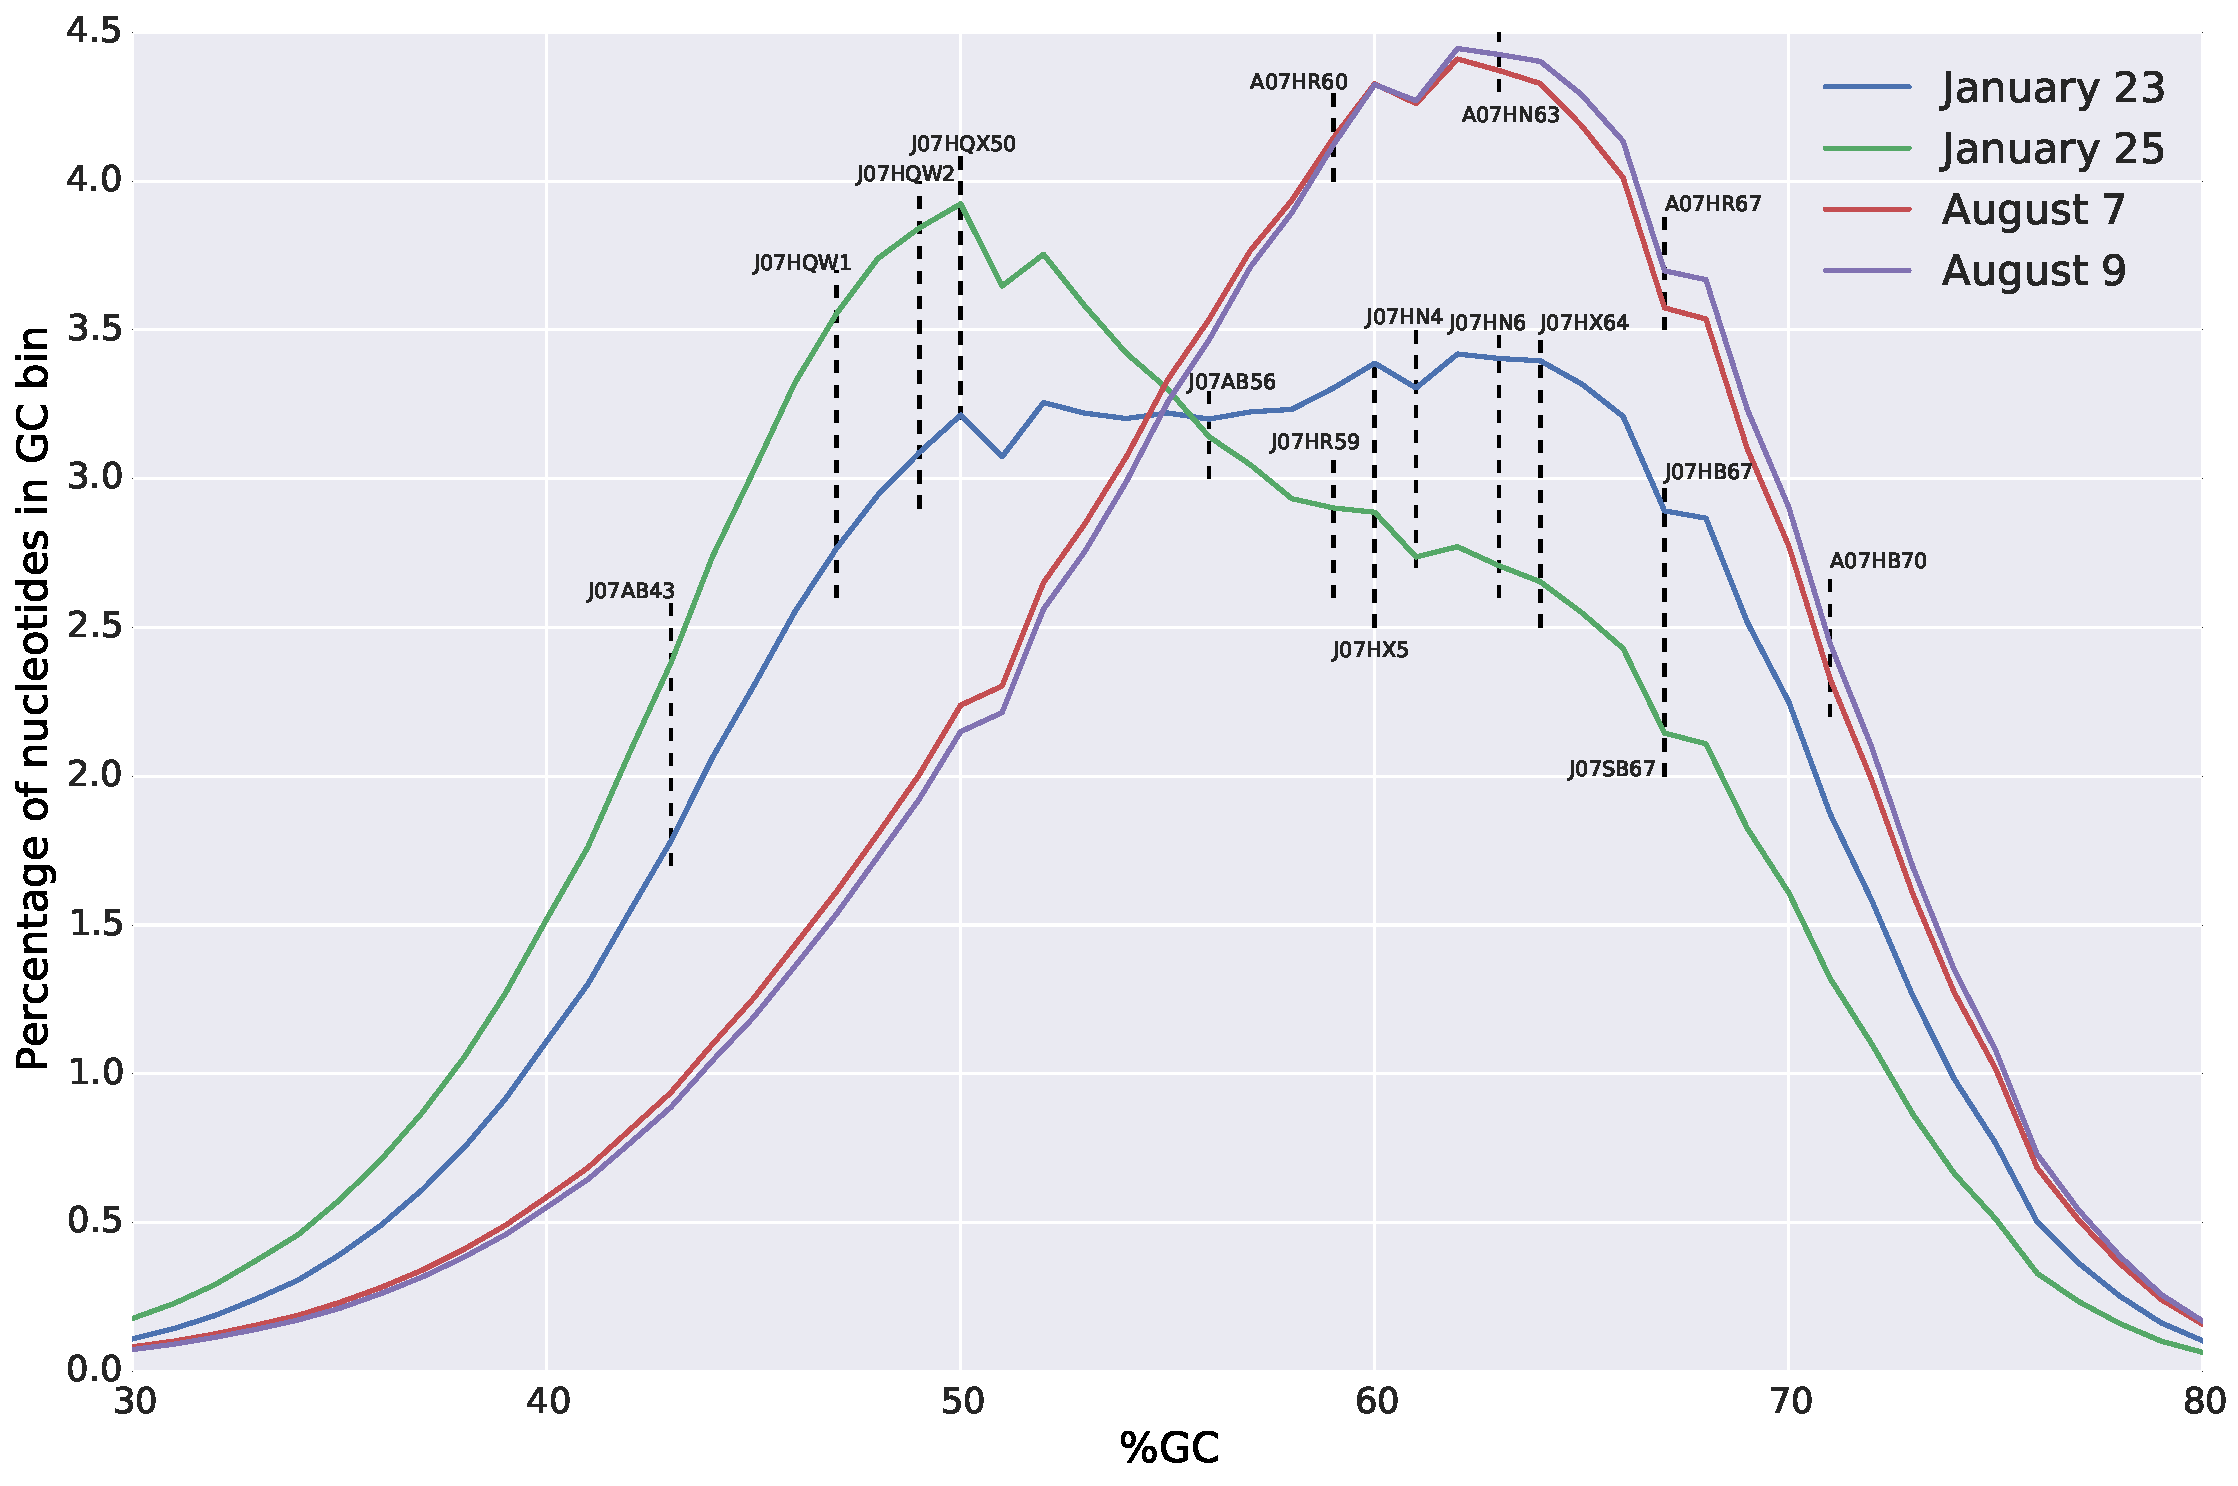
\includegraphics[width=\textwidth]{Chapter5/Figures/GC_content_HiSeqLibs.pdf}
  \caption{Percentage of nucleotides versus G+C content in each of the four sequenced libraries, where each G+C bin has a size of 1\%. Dashed lines indicate the position, based on G+C content, for each of the reference genomes isolated from this community, and that will be used for read mapping (Table \ref{GenomeTable})}
  \label{ReadsGCplot}
\end{figure}
%End of figure

%Table on a new page with facing caption
\clearpage
\thispagestyle{facingcaption}
\begin{table}[h]
\captionsetup{labelformat=prev-page}
\caption{\textbf{Table \ref{LT_chemical}:} Physical and chemical composition of the Lake Tyrrell water samples. Concentrations are given in units of \si{\milli\mole\per\liter}}
\label{LT_chemical}
\end{table}
\clearpage

\begin{sidewaystable}[h]
\ContinuedFloat
\captionsetup{labelformat=empty}
\centering

\begin{tabular}{cccccccccc}

\textbf{Sample} & \textbf{Temp \si{\degreeCelsius}} & \textbf{Total ionic strength} & \textbf{Na} & \textbf{K} & \textbf{Mg} & \textbf{Ca} & \textbf{Cl} & \textbf{Cl} & \textbf{SO42} \\
\hline
\textit{Jan 23} & 21.6 & pH & 5,721 & 4,338 & 32 & 298 & 10 & 5,345 & 123.6 \\
\textit{Jan 25} & 27.9 & 7.09 & 5,950 & 4,163 & 43 & 419 & 11 & 5,291 & 170.5 \\
\textit{Aug 6} & 9.9 & 7.00 & 4,403 & 3,724 & 19 & 126 & 15 & 4,298 & 50 \\
\textit{Aug 8} & 11.5 & 7.01 & 4,060 & 3,557 & 18 & 117 & 14 & 3,830 & 47 \\

\end{tabular}
\end{sidewaystable}

%%%%End of table

%END OF SECTION
\clearpage
\subsection{Read Mapping using Habitat-Specific genomes}

All the reads that passed the quality filters were mapped against the set of habitat-specific genomes (Table \ref{GenomeTable}), from the Lake Tyrrell community. The results indicate differences in the number of reads that each genome recruited, both comparing between samples and between genomes (Table \ref{ReadRecruitmentGenome}). 

In the January samples, the genomes that recruited the most number of reads were the associated with \textit{Haloquadratum} (J07HWQ1 and J07HWQ2), which agrees with previous observations regarding the abundance of these organisms in the Lake Tyrrell community \cite{Podell:2013kx}. The raw number of reads do not provide the best criteria to estimate the relative abundance of each genome in the overall dataset, as these genomes vary in their size. Looking at the coverage of each genome (Table \ref{ReadCoverageGenome}), provides a better proxy for these estimations. The overall coverage, shows similar relative abundances, compared to previous observations \cite{Podell:2013kx}, but it is important to highlight that the number of mapped reads and the coverage do not necessary reflect the real abundance of each organism in the community. Given the strict criteria used for mapping, it is likely that sequences that could be recruited into some of the genomes could be missing. For example, this stringent criteria could explain the low number of reads and low coverage to the genome of \textit{Candidatus} Halobonum turrellensis (G22). This particular organism is an interesting case, because is the only genome that was obtained from an isolate (cultured from August 2007 samples) \cite{Ugalde:2013hb}, but its abundance in the community appears to be very low compared to the other genomes that were recovered via metagenomic assembly. This is a clear example on how in many situations, isolates from an environment are not representative of the most abundant members of a microbial community.

We can estimate how stringent were the mapping criteria, by looking at the sequence identity of each read compared to the mapped genome, and quantify this for each library and genome (Figure \ref{GenomeReadIdentity}). With the exception of the G22 genome, for all genomes and libraries the majority of the reads mapped at a 100\% sequence identity, and it was never lower than 85\%. This already provides an overview on the level of genetic heterogeneity that is present in some of these populations. For example, for the \textit{Haloquadratum} genomes, the majority of the reads mapped at 95\% sequence identity, while in the case of the \textit{Nanohaloarchaea} genomes, we can see that the sequence identity of the recruited reads goes down to 89\%.

%%TABLES AND FIGURES
%Table, reads recruited
\begin{table}[ht!]
  \caption{Total number of recruited reads to each reference genome.}
  \begin{tabularx}{\textwidth}{L{2.2cm}R{2cm}R{3cm}R{3.2cm}R{2cm}}
  \hline
    \textbf{Genome} & \textbf{Jan 23} & \textbf{Jan 25} & \textbf{Aug 07} & \textbf{Aug 09} \\
    \hline
     \textit{J07HWQ1} & 9,712,976 & 10,347,084 & 1,802,421 & 1,385,337 \\
     \textit{J07HWQ2} & 7,311,175 & 9,428,490 & 1,628,137 & 1,301,141 \\
     \textit{J07HQX50} & 922,138 & 1,041,326 & 501,477 & 330,307 \\
     \textit{J07AB56} & 565,197 & 266,831 & 194,445 & 165,278 \\
     \textit{J07AB43} & 760,203 & 486,360 & 63,209 & 64295 \\
     \textit{J07HN4} & 2,149,204 & 2,249,692 & 1,306,287 & 1,089,673 \\
     \textit{J07HN6} & 592,818 & 831,367 & 1,027,472 & 911,341 \\
     \textit{J07HX64} & 4,167,113 & 1,819,023 & 1,202,103 & 1,144,206 \\
     \textit{J07HX5} & 2,106,559 & 1,382,371 & 673,972 & 539,843 \\
     \textit{J07HB67} & 1,124,816 & 1,128,191 & 125,973 & 84,643 \\
     \textit{J07HR59} & 839,856 & 310,496 & 2,105,598 & 1,693,772 \\
     \textit{A07HB70} & 550,429 & 277,030 & 1,970,106 & 1,866,967 \\
     \textit{A07HR67} & 563,043 & 270,602 & 2,166,129 & 1,680,150 \\
     \textit{A07HN63} & 547,808 & 786,856 & 1,126,032 & 1,003,322 \\
     \textit{A07HR60} & 2,126,700 & 758,549 & 5,405,933 & 4,362,857 \\
     \textit{G22} & 62,983 & 39,696 & 72,261 & 66,778 \\
     \textit{J07SB} & 797,957 & 211,306 & 737,471 & 673,630 \\     
  \textit{Unmapped} & 45,344,829 & 31,913,858 & 51,012,461 & 44,849,506 \\
  \end{tabularx}
  \label{ReadRecruitmentGenome}
\end{table}

%Table, reads coverage
\begin{table}[ht!]
  \caption{Genomes coverage (expressed as X-fold) in each of the libraries.}
  \begin{tabularx}{\textwidth}{L{2.2cm}R{2cm}R{3cm}R{3.2cm}R{2cm}}
  \hline
    \textbf{Genome} & \textbf{Jan 23} & \textbf{Jan 25} & \textbf{Aug 07} & \textbf{Aug 09} \\
    \hline
     \textit{J07HWQ1} & 274.9 & 292.7 & 51.0 & 39.2 \\
     \textit{J07HWQ2} & 200.2 & 258.0 & 44.5 & 35.6 \\
     \textit{J07HQX50} & 30 & 33.9 & 16.3 & 10.7 \\
     \textit{J07AB56} & 45.5 & 21.5 & 15.6 & 13.2 \\
     \textit{J07AB43} & 61.2 & 39.1 & 5.1 & 5.2 \\
     \textit{J07HN4} & 72.4 & 75.7 & 44.0 & 36.7 \\
     \textit{J07HN6} & 22.8 & 31.9 & 39.4 & 35.0 \\
     \textit{J07HX64} & 135.5 & 59.1 & 39.1 & 37.2 \\
     \textit{J07HX5} & 100.5 & 65.9 & 32.1 & 25.7 \\
     \textit{J07HB67} & 40.9 & 41.0 & 4.6 & 3.1 \\
     \textit{J07HR59} & 38.6 & 14.2 & 96.7 & 77.7 \\
     \textit{A07HB70} & 22.1 & 11.1 & 79.1 & 74.9 \\
     \textit{A07HR67} & 18.8 & 9.0 & 72.2 & 56.0  \\
     \textit{A07HN63} & 22.2 & 31.9 & 45.7 & 40.7 \\
     \textit{A07HR60} & 72.0 & 25.7 & 183.1 & 147.7 \\
     \textit{G22} & 1.6 & 1.0 & 1.9 & 1.7 \\
     \textit{J07SB} & 40.1 & 10.6 & 37.1 & 33.8 \\     
  \end{tabularx}
  \label{ReadCoverageGenome}
\end{table}


%Figures for this section

%Figure, Genome Identity Plots
\begin{figure}[!hbtp]
  \centering
  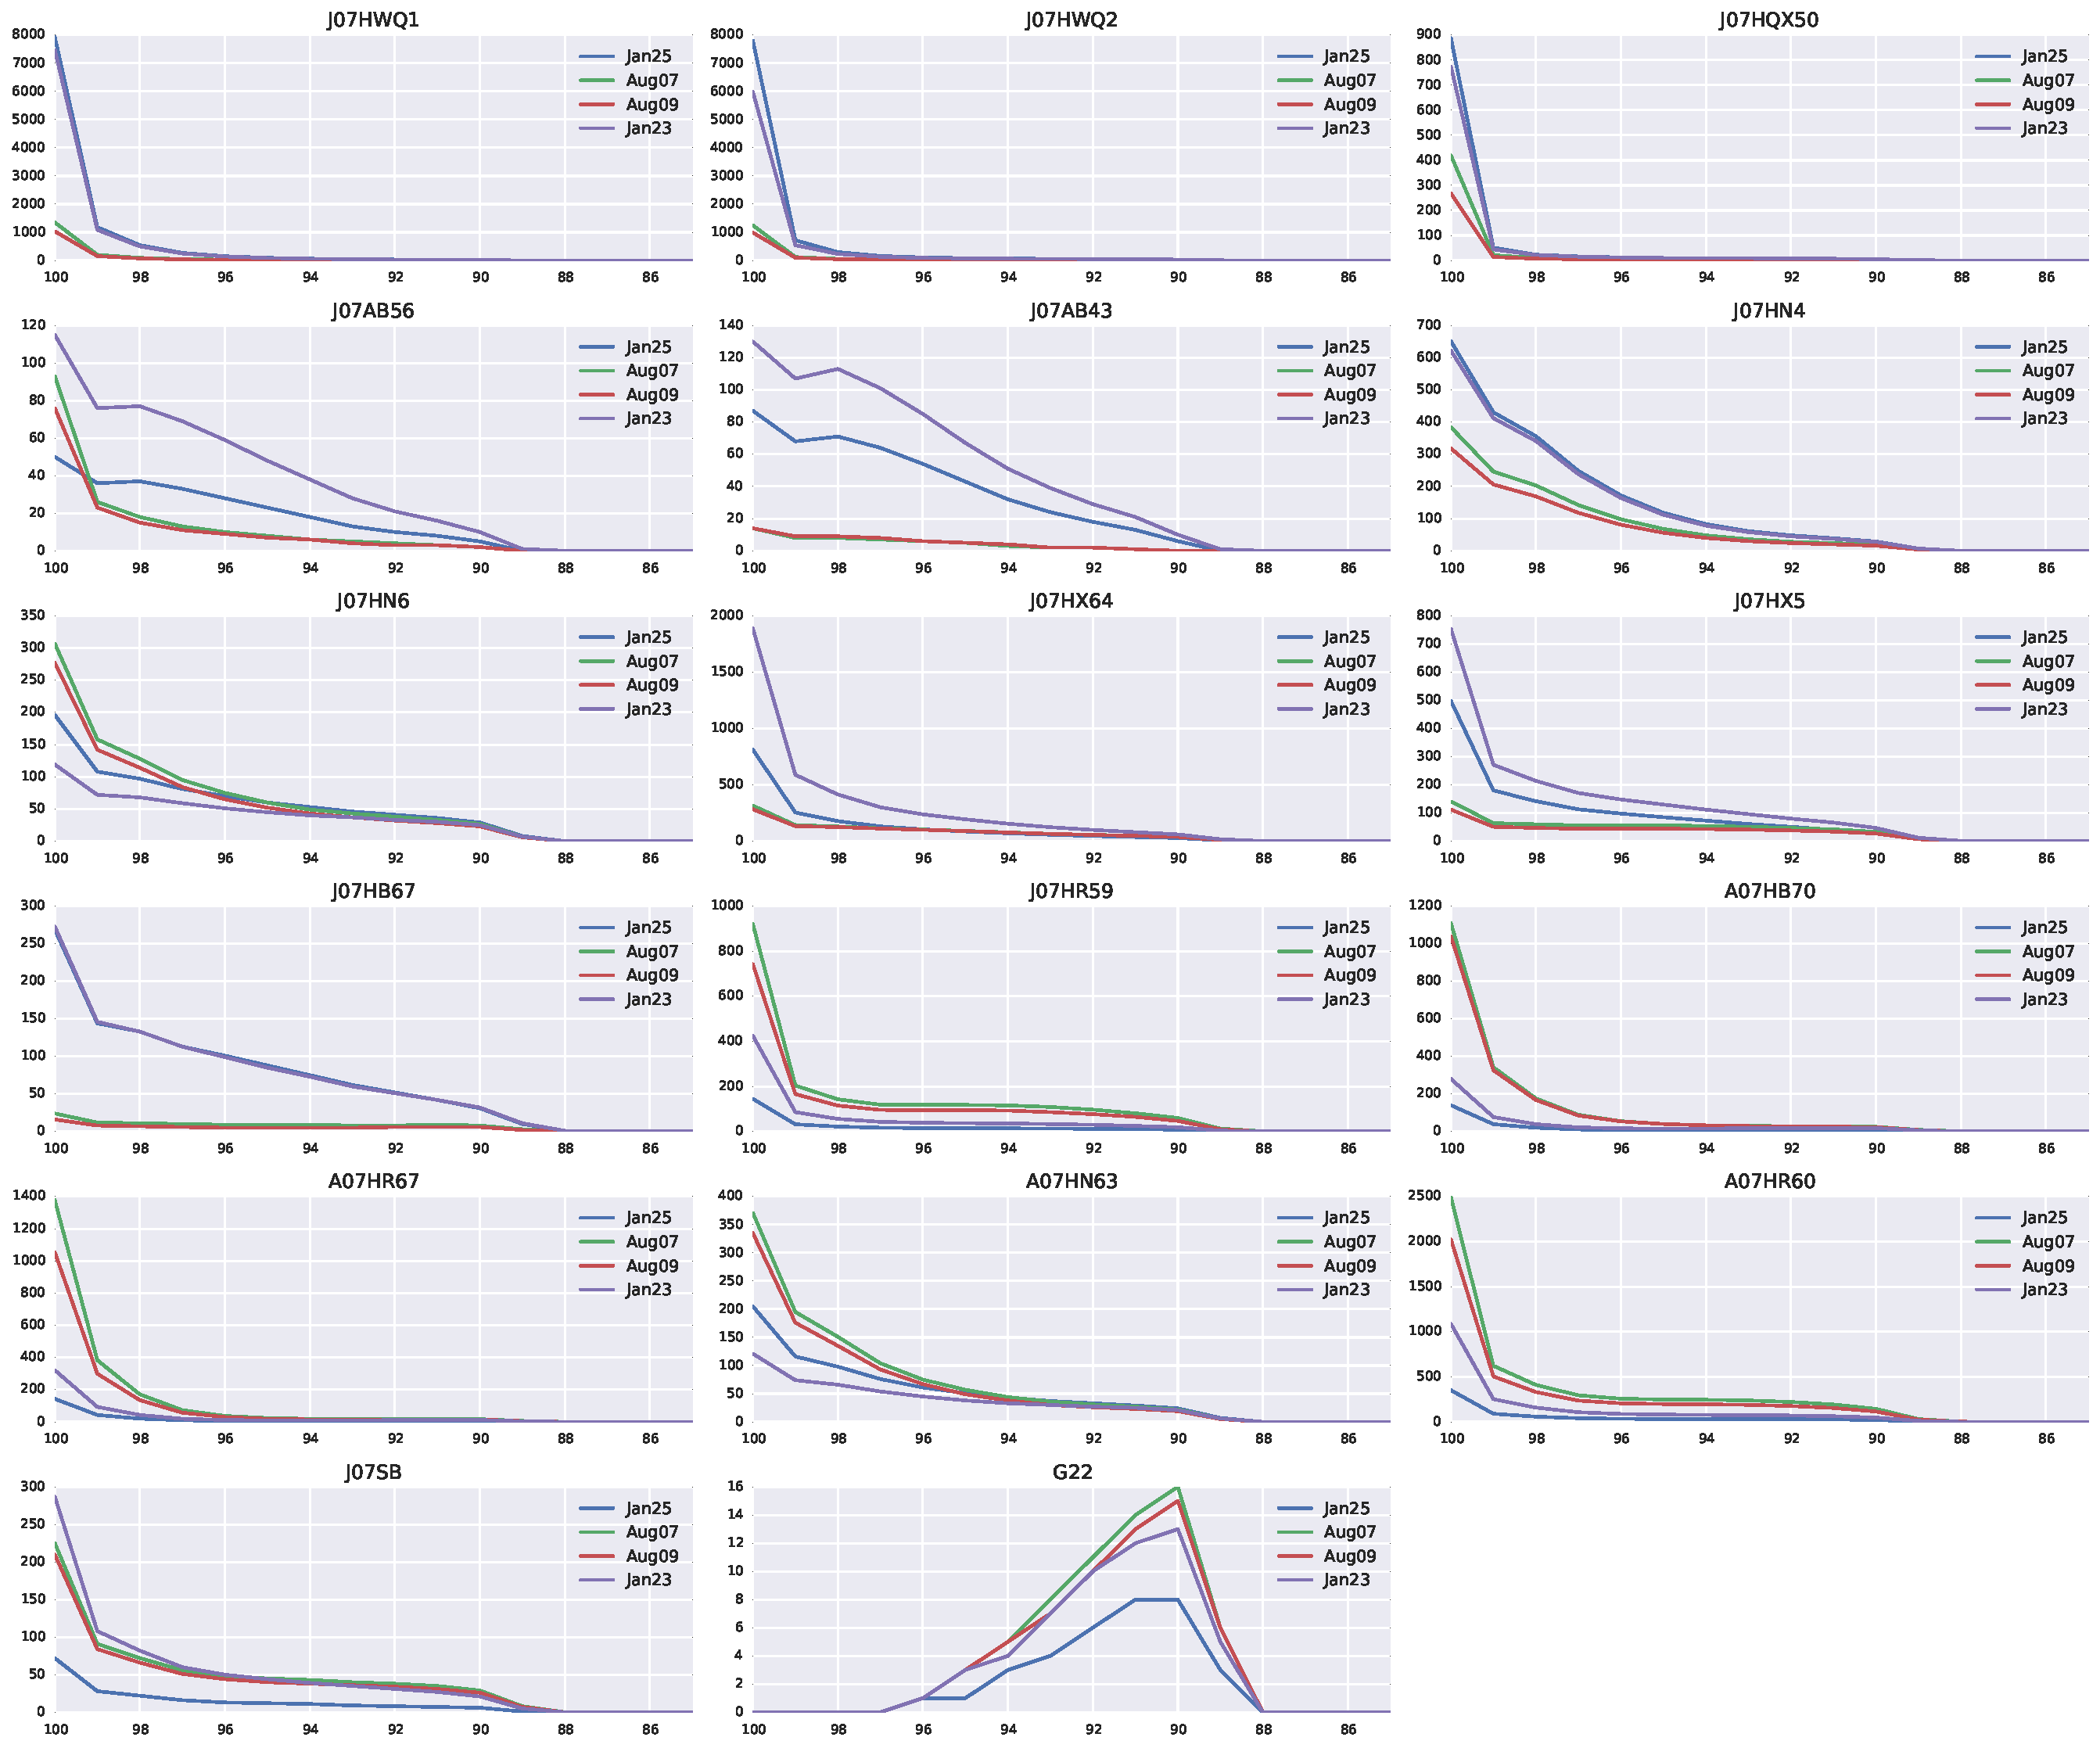
\includegraphics[width=\textwidth,height=0.9\textheight,keepaspectratio]{/Users/juan/Dropbox/GeneticVariationLT/Figures/GenomeIdentityPlots.pdf}
  \caption{Total number of recruited reads, grouped by sequence identity. The X axis shows the identity of the read to the reference genome (\%), while the \textbf{Y} axis shows the number of reads recruited at that identity (thousands of reads).}
  \label{GenomeReadIdentity}
\end{figure}


%%%NEW SUBSECTION
\clearpage
\subsection{Taxonomic Classification of Mapped and Unmapped Reads}

Before going on a more detailed analysis of the genetic heterogeneity present in the Lake Tyrrell microbial community, we need to address the results of the read mapping to the reference genomes. With the deep level of coverage of the community achieved with the four libraries (~6 billion nucleotides in each library), this dataset represents not only the most abundant members of the community, as represented in the reference genomes used for mapping, but also allows the possibility of discovering novel organisms in the unmapped sequences \cite{Narasingarao:2012kp,Albertsen:2013gpa}. To provide an overview of the differences between the set of mapped and unmapped reads, the software Phylosift  \cite{Darling:2014ej} was used to generate a taxonomic classification of both sets of reads, based on presence of phylogenetic markers. An example of these results is shown on Figure \ref{Jan23_Tax}, for the sample collected on January 23. In the case of the mapped reads (Figure \ref{Jan23Mapped}), as expected the majority of the reads were classified as \textit{Haloquadratum}, followed by the \textit{Nanohaloarchaea}. There are also hits to organisms that were not present in the reference genomes, such as \textit{Natronema}, something that can be explained by the size of the reads (100 nt. long), which could generate spurious hits with other related organisms. In contrast, the set of unmapped reads (Figure \ref{Jan23Unmapped}) shows a broad diversity of taxonomic groups, including groups not present in the reference genomes, such as \textit{Natronomonas}, but also groups that are present, like \textit{Salinibacter} and the \textit{Nanohaloarchaea}. This suggests that the diversity of these groups is higher than expected, and is not represented only by what is present on the reference genomes used for mapping. This also highlights the potential for the recovery of novel genomic sequence, either from this group, or from novel representatives from other Archeal genera.

To evaluate the differences in taxonomic composition between the set of mapped and unmapped reads, the Phylosift results were evaluated using an edge principal component analysis (EPCA), which takes in account the phylogenetic composition (similar to Unifrac distances) \cite{Matsen:2011wn}. Looking at the first two components (Figure \ref{EPCA_results}), shows that based on the predicted taxonomic composition of all the libraries, the reads separate between the mapped and unmapped groups, in addition of a separation by sample (January versus August) in the case of the unmapped reads. Technical problems limited the analysis of two of the datasets from the mapped reads, so the only comments that can be currently made with certainty are about the separation between the unmapped and mapped reads.

As mentioned earlier, the taxonomic analysis suggests that indeed there are novel groups in the unmapped reads, that are not represented in the reference genomes. This also includes the presence of viral sequences, which were not taking in account in the taxonomic analysis, and could compromise a large percentage of the sequences present in each of libraries \cite{RodriguezBrito:2010in,Emerson:tk}. Further work, should include viral markers in the taxonomic classification, as well as mapping the sequences against available viral genomes. Nevertheless, by using the current set of reference genomes, some of the most abundant members of this community are being explored, and this information can be used to explore the genetic diversity present in the community, by using a set of already validated habitat-specific genomes.

%Figure Phylosift results
\begin{figure}[!hbtp]
\centering
\subfloat[Mapped reads]{
    \label{Jan23Mapped}
    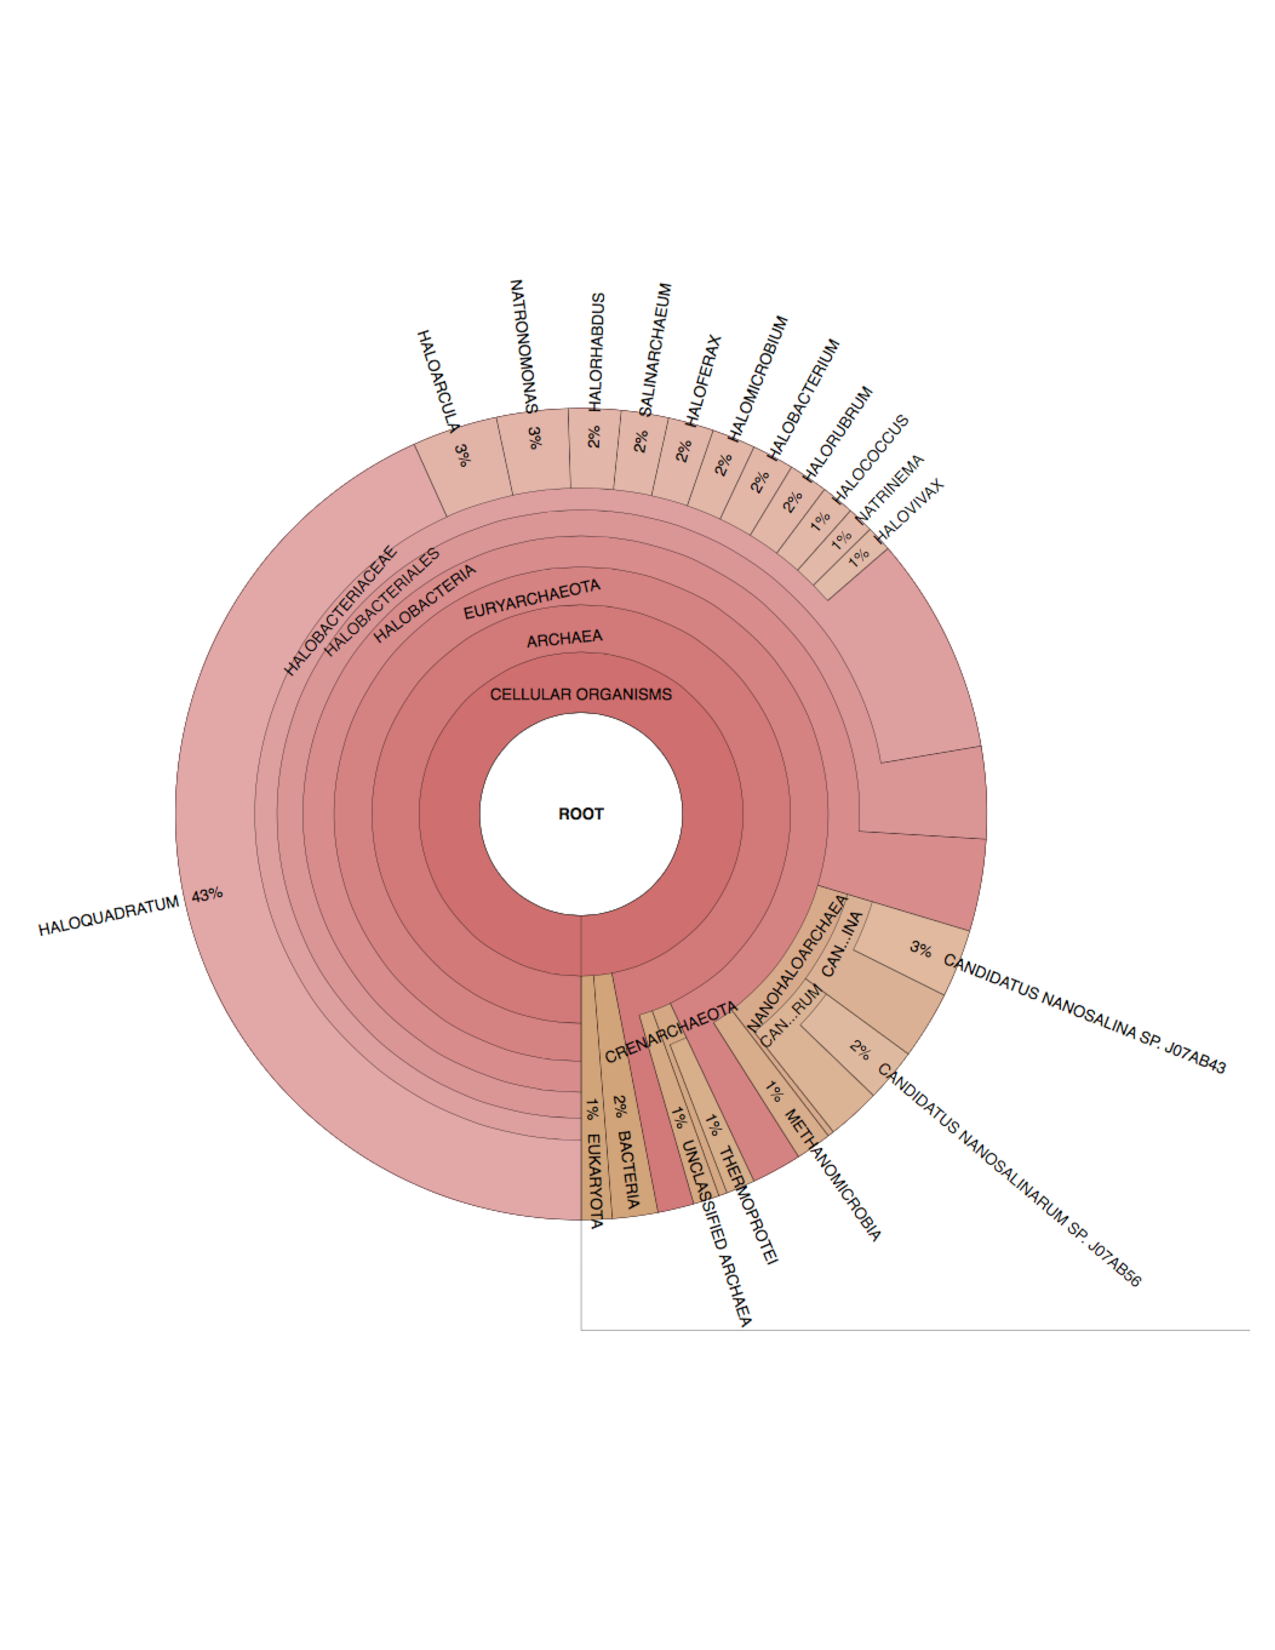
\includegraphics[width=0.7\textwidth]{Chapter5/Figures/Jan23_Mapped.pdf}
    }
    \hfill
\subfloat[Unmapped reads]{
    \label{Jan23Unmapped}
    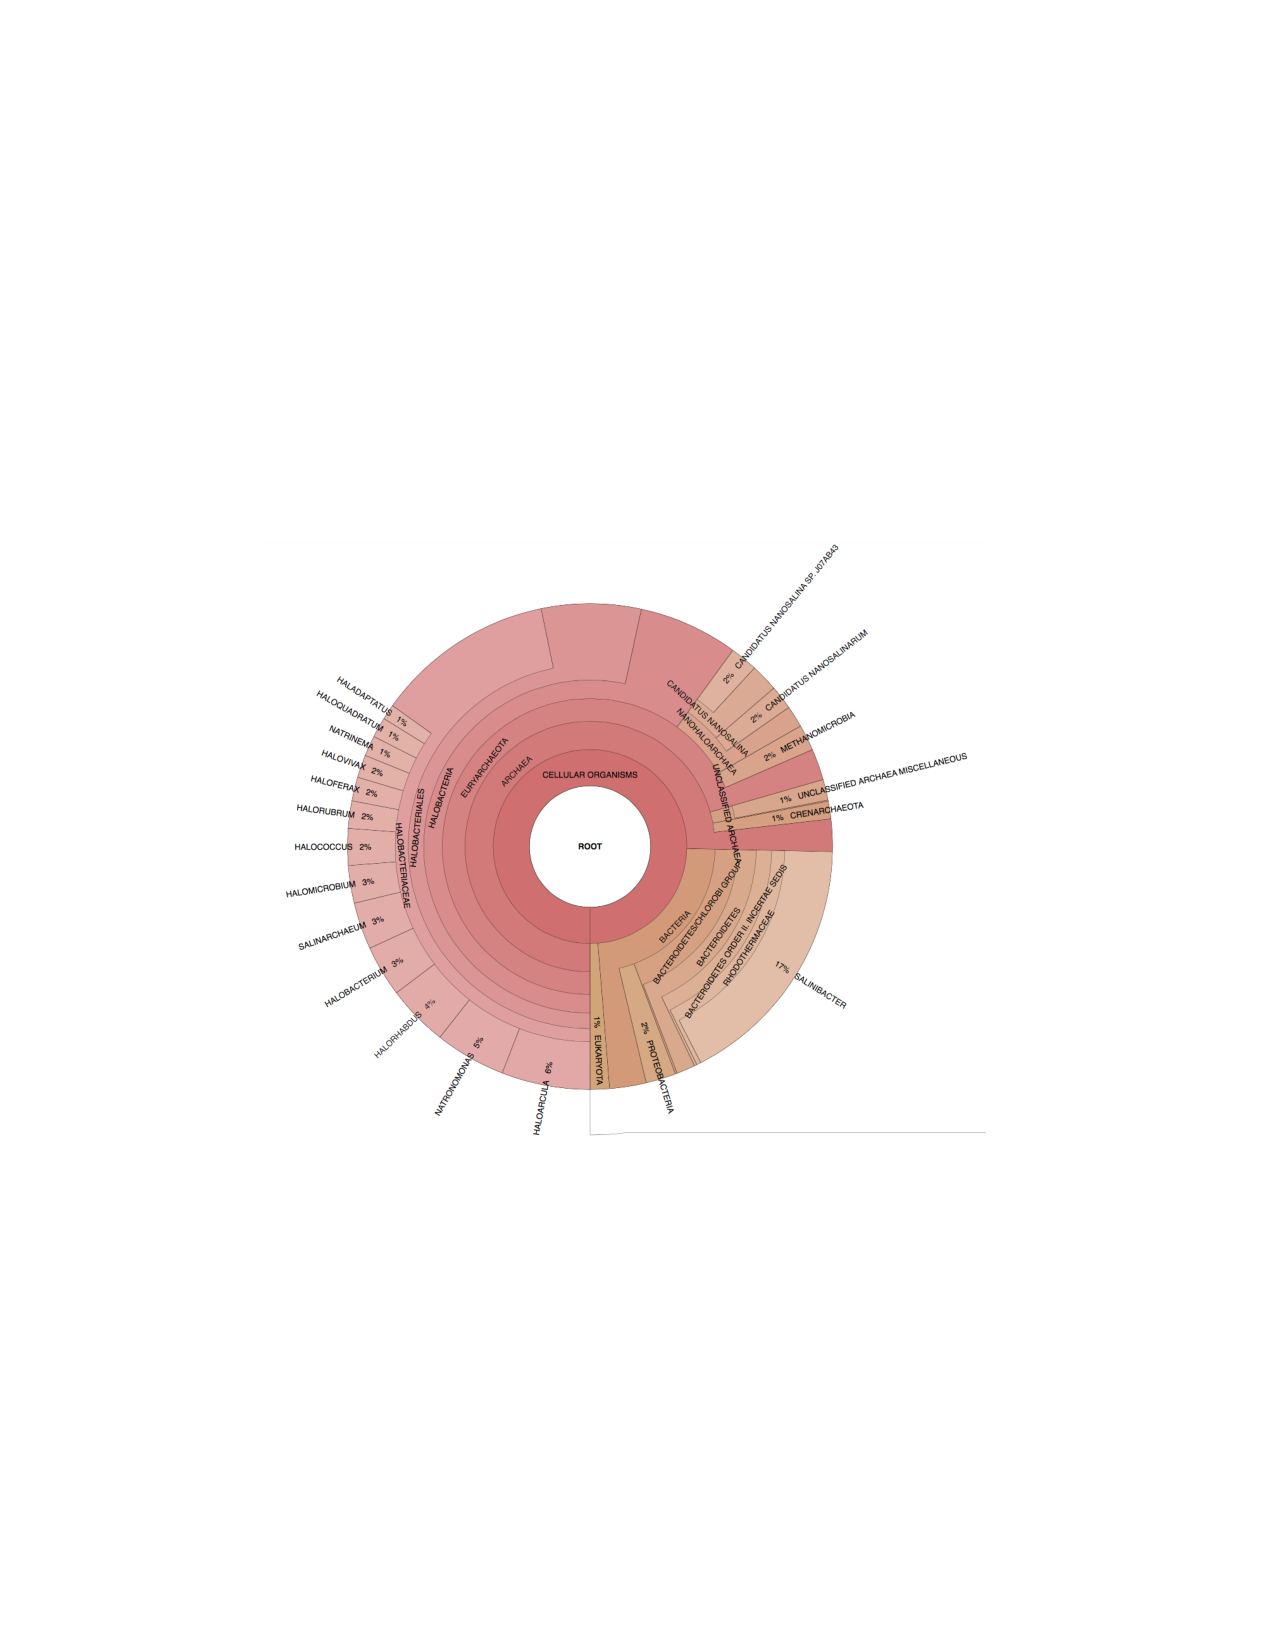
\includegraphics[width=0.7\textwidth]{Chapter5/Figures/Jan23_Unmapped.pdf}
    }
    \caption{Taxonomic classification of the mapped and unmapped reads using Phylosift \cite{Darling:2014ej}}
    \label{Jan23_Tax}
\end{figure}

%Figure Phylosift EPCA
\begin{figure}[hbt]
  \centering
  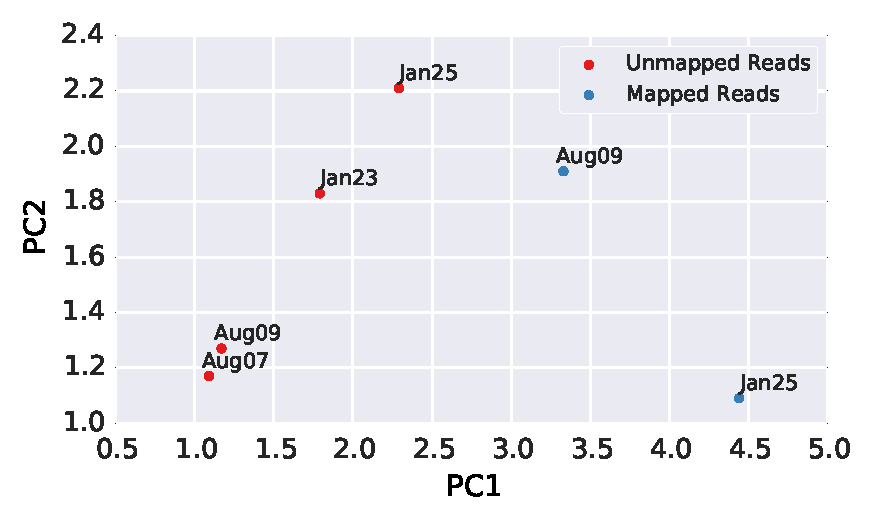
\includegraphics[width=\textwidth]{Chapter5/Figures/Unmapped_Mapped_EPCA.pdf}
  \caption{Edge principal component analysis (EPCA) of the taxonomic classification of each library.}
  \label{EPCA_results}
\end{figure}


%%%%%%%%%%%%%%%%%%%%%%
\clearpage
\subsection{Differential coverage of genomes and genes}

As mentioned in the previous sections, the number of mapped reads to each of the reference genomes and the genome coverage (Tables \ref{ReadRecruitmentGenome} and \ref{ReadCoverageGenome}), suggests differences in the relative abundance of some of the populations between sampling times (January versus August). For example, the genomes of \textit{Haloquadratum} microorganisms (J07HWQ1 and J07HWQ2), recruited more reads from the January samples than from the August sample. By comparison, the reference genomes that were assembled from August samples \cite{Podell:2013fp}, like A07HR60, recruited more reads from the August libraries. However, by just looking at the total coverage of a genome, does not provide a complete picture, because it is possible that some regions have higher coverage than other ones.

This differential coverage can be analyzed from two perspectives, if we consider the comparison between January and August samples (combing the two individual dates for each season). From the analysis within each month, some regions may show depths of coverage that are lower than the rest of the genome. This suggest the presence of multiple strains within that particular organism, where only some of the members of the population have that particular region \cite{Pasic:2009bo,Legault:2006kh,Allen:2005dg}. This has been shown in the case of \textit{Haloquadratum} \cite{Legault:2006kh} and \textit{Salinibacter} \cite{Pasic:2009bo}, using reference genomes and mapping reads from different environments, showing the presence of these metagenomic islands. The second perspective, is to compare the coverage of each genome between the January and August samples, looking for regions of differential coverage (higher in one sample, versus the other).

To evaluate this differential coverage within and between samples, the identity and coverage of all the reads along each one of the reference genomes was evaluated. This was done for both January and August samples (Appendix \ref{AppendixCoverage}). This approach allows to identify regions with low coverage, suggesting a region only present on a subset of the strains of the populations, as well as the differential coverage between January and August. In addition, changes in the relative abundance of each gene were incorporated, with the goal of identifying differential covered genes (not only regions). By looking at the individual genes this allows to identify possible functional processes that are more abundant in one sample versus the other.

As expected, the coverage plots indicates that for some of the reference genomes, there are difference in the coverage along the genomic sequence (Appendix \ref{AppendixCoverage}. For example, in the case of the \textit{Nanohaloarchaea} J07AB56 (Figure \ref{J07AB56coverage}), there are two regions that appear with a higher coverage in the August samples, with genes that have a differentially higher coverage in this sample. Looking in more detail, within the first region, genes encoding for hypothetical proteins (several of them with homology to halophages), DNA-primases and replication proteins, were found. This region is located within the largest scaffold of the J07AB56 genome, suggesting that is indeed part of the genome. A possible hypothesis is that this region constitute a halovirus that is carried as a prophage, but was released on the August sample (maybe due to environmental changes) \cite{Porter:2007jw}. The second region, has genes encoding for defense mechanisms, such as ABC transporters, oxidoreductases, besides the usual hypothetical proteins.

A summary of the differential recruitment of the reads at the gene level is shown on Figure \ref{CoverageGenes}), which indicates that in the case of the reference genomes that were recovered from the January samples, the majority of its genes indeed recruited to reads from the January Illumina libraries. Some exceptions to this are in the \textit{Halonotius} J07HN6 genome, that has a large fraction of the genes recruiting more reads from the August libraries than from the January ones. It is possible that indeed this organism is present and abundant in the August samples, but it was not previously assembled. Also the \textit{Halonotius} J07HN6 and A07HN63 are very similar \cite{Podell:2013fp}, which could also explain the higher differential coverage.

The idea of looking at the differential coverage of the genomes, and comparison between multiple samples, is not new in the literature \cite{DyallSmith:2011tu,Pasic:2009bo}, but provides an broad picture of the possible strain variation that is present for each of the population under study. To our knowledge, the idea of using RPKM values, commonly used in gene expression studies \cite{Mortazavi:2008jj}, and apply it to comparisons to metagenomic samples, is indeed a novel one. Although a broad picture of the differences was presented in here, further work will focus in specific populations, such as the \textit{Haloquadratum} genomes, including also the use of available isolate genomes \cite{DyallSmith:2011tu}.

%Figure Gene differences season
\begin{figure}[!hbtp]
  \centering
  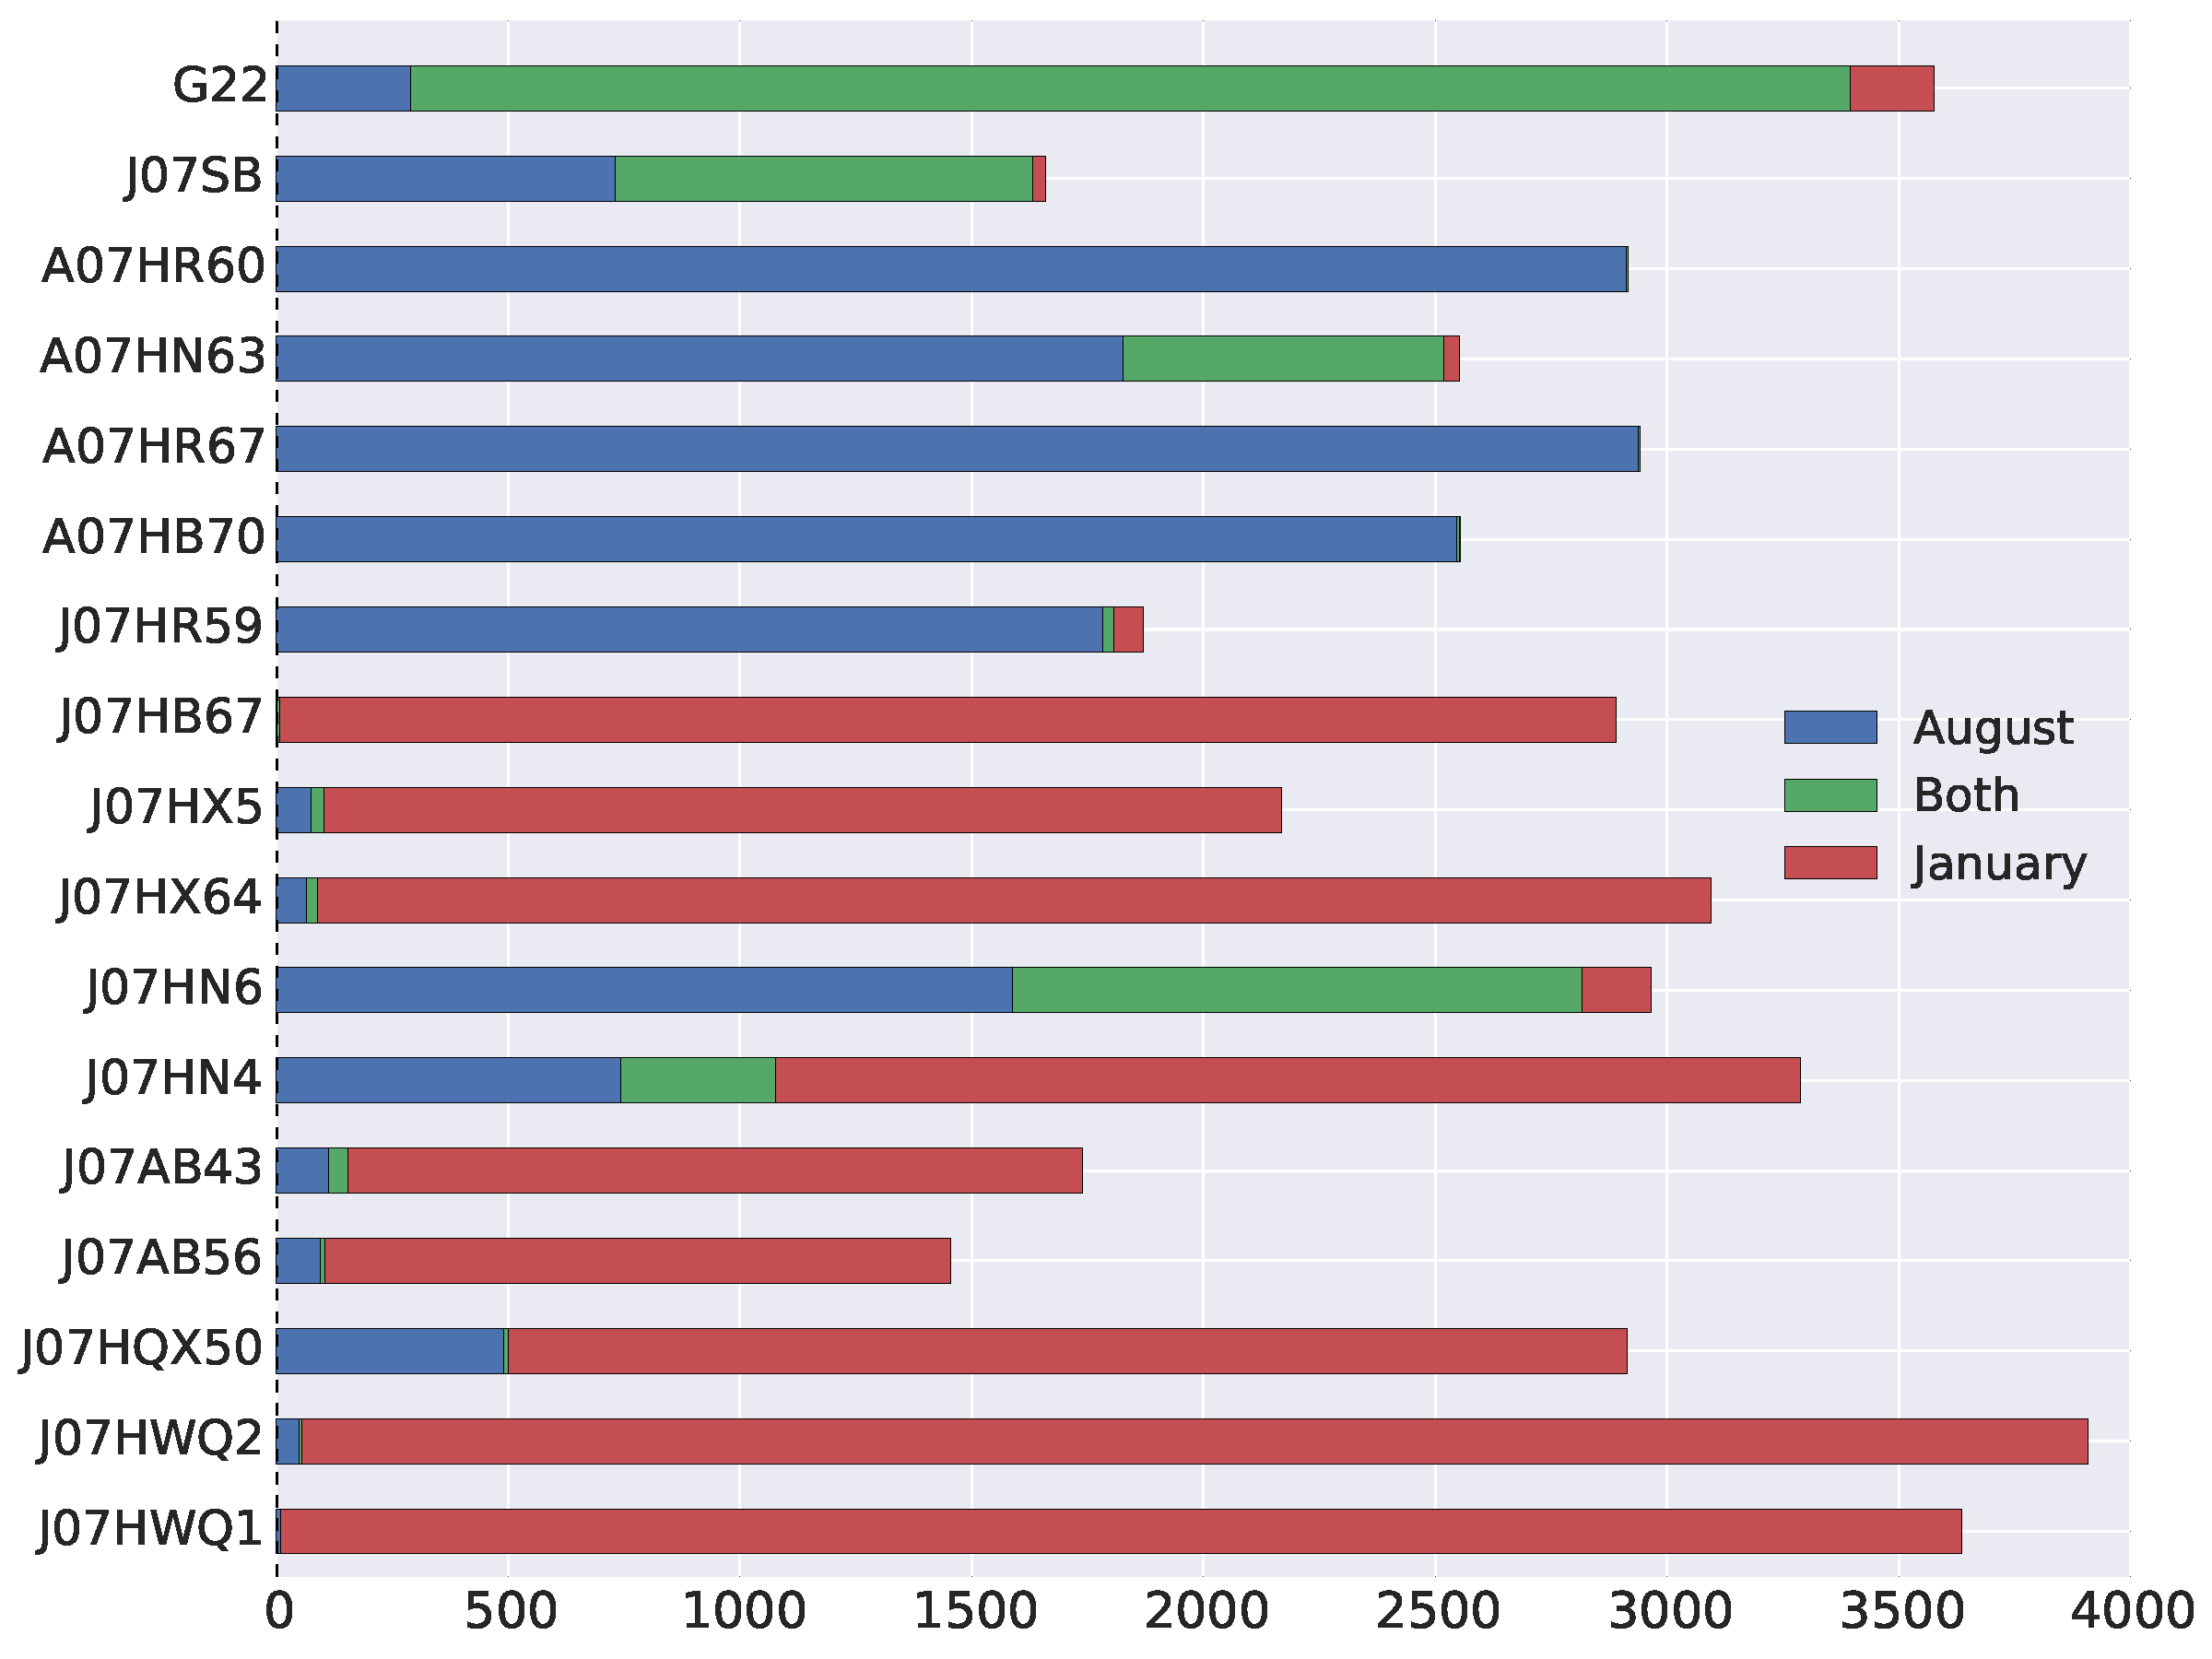
\includegraphics[width=0.7\textwidth]{Chapter5/Figures/GeneDifferencesSeason.pdf}
  \caption{Number of genes that differentially recruited reads from either the January or August libraries, in each of the reference genomes. A two-tailed Fisher Exact test (p-value $<$ 0.05) was used to determined the differences between samples. \textit{Both}, indicates genes that were not found to be significantly more abundant in either of the samples.} 
  \label{CoverageGenes}
\end{figure}

%%%%%%%%%%%%%End of Section
\clearpage
\subsection{Fine-scale Genetic Variation: Single Nucleotide Polymorphisms (SNPs)}

The genetic heterogeneity that is present in each of the reference populations, can be explored in more detail by leveraging on the information provided by the reads and the high depth of coverage of each of the genomes (with the exception of G22). With this, it is possible to quantify the nucleotide variation in each genome (single nucleotide polymorphisms, SNPs) and evaluate the effects of such variation at the functional level. Other types of variations, such as insertions, deletions and structural variants, can be analyzed as well, but the current goal is to evaluate the evolutionary forces that are generating such variation, so the emphasis will be on the polymorphisms that act on protein-coding sequences.

For variant calling, only high-quality SNPs were considered in the analysis, filtering the alignment files previous to SNP calling with Freebayes. Only those sites with a quality score of 20 or more and mapping quality score of 30 or more were selected in the analysis, similar as how it has been done in other studies \cite{Schloissnig:2012hx}

The number of SNPs/Kb on each of the genomes is shown on Table \ref{SNPS_KB}, indicating differences on the number of SNPs when comparing the different references. Within each of the genomes, there are small differences within each season sample (January 23 \& January 25, August 7 \& August 9), but there are differences between the January and August samples. The \textit{Nanohaloarchaea} genomes, exhibit the largest number of SNPs/Kb among all the genomes, in the January libraries, but is lower on the August libraries. Comparing the number of SNPs/Kb found on each library, we can visualize that all four of them are within similar ranges (Figure \ref{BoxplotSNPsKB}), with averages between 4-5 SNPs/Kb.

Although from the visual inspection of Table \ref{SNPS_KB}, it does not appear that there is any relationship between those genomes that recruited more reads and the number of SNPs, this needs to be evaluated. When comparing the depth of coverage of each reference genome, versus the number of SNPs/Kb found in each of the libraries (Figure \ref{SNPsCoverage}), there is no relationship between these two variables. This was confirmed by testing with the Spearman correlation coefficient for the combined libraries (0.16, \textit{pvalue}:0.21). This strongly suggests that the differences in SNPs numbers are due to the genetic diversity found in each of these reference genomes, where organisms like the \textit{Nanohaloarchaea} J07AB43 and J07AB56, have higher rates of genetic diversity (more strain diversity) compared to organisms like J07HWQ1 or J07HWQ2.

The effect of each variation within the genome, can be evaluated in more detail by quantifying those SNPs that were intergenic or located within a coding region. In the latter case, this variation could be either synonymous (no amino acid change) or non-synonymous (change in the resulting amino acid). For each of the genomes, no differences between libraries in the percentage of intergenic, non-synonymous and synonymous SNPs (Figure \ref{SNPsummary}) were observed, with the exception of the G22 genome, but the overall coverage and percentage of SNPs for this genome is low. The distribution of SNPs for all the genomes (Figure \ref{BoxPlotSNP}), shows that the majority of the SNPs are located in coding sequences, and are synonymous. Also it is interesting to observe the dispersion on the data, where for the case of the non-synonymous SNPs, the distribution goes between 20-30\%, while in the case of intergenic SNPs moves between 15-37\%. These can be observed more in detail on Table \ref{TypeSNP_SummaryGenome}, where on one extreme we have genomes from the \textit{Haloquadratum} group with over ~30\% of the SNPs within intergenic regions, and on the other side the \textit{Nanohaloarchaea}, with ~10\% of the SNPs within intergenic regions. This can be explained by the differences in genome size, where \textit{Haloquadratum} organisms have large genomes (over 3 Mb.), and the \textit{Nanohalorachaea} have smaller genomes (1.8 Mb), with reduced intergenic space \cite{Narasingarao:2012kp,Podell:2013kx}. Overall, the percentage of non-synonymous substitutions for all the genomes was similar, something expected given the chararacteristics of this type of change, which modifies the amino acid sequence and can led to non-functional organisms. Compared to values observed in other metagenomic studies (focusing only on a few species), the trends observed are similar, with higher rates of synonymous substitutions compared to non-synonymous ones \cite{Simmons:2008by}.

The sampling strategy allows us to ask two different questions in terms of the temporal variation between the samples. First, a variation within each sampling month (January and August), between the samples collected two days apart. The second comparison is between the two different seasons (January vs August). By looking at the SNPs found on each of the samples, we can look if the SNPs found are unique to each one of the libraries, or there are similarities between time points. We can visualize the differences using Venn diagramas, comparing the different sampling dates. The comparison between the January dates (23 versus 25) (Figure \ref{VennJan}), shows that in all the reference genomes, the majority of the SNPs is shared between the two samples days. G22 is an exception, due to its low coverage. A similar trend is observed in the comparison of the August 7 and August 9 libraries (Figure \ref{VennAug}), but in here the \textit{Nanohaloarchaea} genomes (J07AB56 and J07AB43) have differences between the two dates. These suggests that different populations of these organisms may be found in these two samples, but further analysis (focusing only in these two populations), is needed to answer this question, and evaluate if these differences are indeed due do difference in population structure for these organisms \cite{Schloissnig:2012hx,Shapiro:hi,Vos:2011ux}. Both dates (January versus August) were compared using the combined set of SNPs. This is the sample comparison where the attention will be focused in the rest of this Chapter. Interestingly, the majority of the SNPs appear to be shared between the two samples, with small differences in the case of the \textit{Nanohaloarchaea}, with unique SNPs present in the January sample. This suggests that the populations found in January could be very similar to the ones present in August \cite{Doolittle:2012hf}, the same strains could be present, but what changes is the abundance of the members of the community, something that is supported by the previous analysis of the reads that mapped to each reference genome. Exploring this phenomenon requires focusing on a few organisms, comparing not only these assembled genomes, but also genomes from other environments and/or isolates if available. In particular, measurements of nucleotide diversity, fixation index and McDonald-Kreitman tests \cite{Schloissnig:2012hx,Simmons:2008by} to evaluate differences at the population level between the members of the community. Nevertheless, the idea of both population being similar, with only differences in their abundances, is an interesting one. The slow growth reate of some of the organisms found in hypersaline communities \cite{DyallSmith:2011tu} (at least in laboratory studies), may suggest that samples of seven months apart is not long enough to provide a temporal picture of the evolution of the population structure within this ecosystem, which contrasts with has been observed for viral communities in hypersaline communities, where temporal variation has been observed in different hypersaline ecosystems \cite{RodriguezBrito:2010in,Emerson:2012gh}.

%%Tables and Figures

%Table count of snps
\begin{table}[ht]
  \caption{Count of number of SNPs per kilobase in each of the Illumina libraries for the reference genomes.}
  \begin{tabularx}{\textwidth}{L{2.2cm}R{2cm}R{3cm}R{3.2cm}R{2cm}}
  \hline
    \textbf{Genome} & \textbf{Jan 23} & \textbf{Jan 25} & \textbf{Aug 07} & \textbf{Aug 09} \\
    \hline
     \textit{J07HWQ1} & 3.83 & 3.81 & 3.75 & 3.70 \\
     \textit{J07HWQ2} & 2.51 & 2.52 & 3.28 & 2.46 \\
     \textit{J07HQX50} & 1.44 & 1.44 & 1.42 & 1.39 \\
     \textit{J07AB56} & 10.10 & 9.71 & 4.95 & 5.21 \\
     \textit{J07AB43} & 10.75 & 10.64 & 7.30 & 7.19 \\
     \textit{J07HN4} & 9.09 & 9.09 & 9.01 & 9.01 \\
     \textit{J07HN6} & 2.87 & 2.61 & 2.85 & 2.81 \\
     \textit{J07HX64} & 9.52 & 9.43 & 9.35 & 9.26 \\
     \textit{J07HX5} & 9.26 & 9.17 & 9.09 & 9.01 \\
     \textit{J07HB67} & 9.09 & 9.17 & 6.45 & 5.24 \\
     \textit{J07HR59} & 1.36 & 1.15 & 1.54 & 1.51 \\
     \textit{A07HB70} & 7.19 & 7.04 & 7.30 & 7.30 \\
     \textit{A07HR67} & 5.85 & 5.71 & 5.92 & 5.92 \\
     \textit{A07HN63} & 1.72 & 1.98 & 2.12 & 2.10 \\
     \textit{A07HR60} & 3.79 & 3.69 & 3.91 & 3.89 \\
     \textit{G22} & 0.04 & 0.03 & 0.03 & 0.03 \\
     \textit{J07SB} & 6.06 & 5.65 & 6.10 & 6.10 \\     
  \end{tabularx}
  \label{SNPS_KB}
\end{table}

%TABLE SUMMARY TYPE OF SNPs

\begin{table}[ht]
  \caption{Summary of type of SNP on each genome}
  \begin{tabularx}{\textwidth}{L{2.1cm}R{2.3cm}R{3cm}R{3.8cm}}
  \hline
    \textbf{Genome} & \textbf{Intergenic} & \textbf{Synonymous} & \textbf{Non-Synonymous}\\
    \hline
     \textit{J07HWQ1} & 36.90 & 38.56 & 24.55 \\
     \textit{J07HWQ2} & 37.31 & 34.48 & 28.22 \\
     \textit{J07HQX50} & 31.32 & 36.95 & 31.73 \\
     \textit{J07AB56} & 10.67 & 65.96 & 23.37 \\
     \textit{J07AB43} & 10.30 & 64.02 & 25.68 \\
     \textit{J07HN4} & 15.27 & 66.28 & 18.45 \\
     \textit{J07HN6} &  19.98 & 55.62 & 23.40\\
     \textit{J07HX64} & 18.98 & 51.18 & 29.84 \\
     \textit{J07HX5} & 20.72 & 53.88 & 25.41 \\
     \textit{J07HB67} & 12.06 & 60.65 & 27.29 \\
     \textit{J07HR59} & 23.78 & 53.89 & 22.33 \\
     \textit{A07HB70} & 22.38 & 49.23 & 28.40 \\
     \textit{A07HR67} & 20.75 & 55.58 & 23.67 \\
     \textit{A07HN63} & 21.55 & 54.69 & 23.76 \\
     \textit{A07HR60} & 26.79 & 49.54 & 23.67 \\
     \textit{G22} & 15.86 & 65.34 & 17.80 \\
     \textit{J07SB} & 15.67 & 59.60 & 24.74 \\     
  \end{tabularx}
  \label{TypeSNP_SummaryGenome}
\end{table}

%FIgures. SNPs versus depth of coverage
\begin{figure}[h]
  \centering
  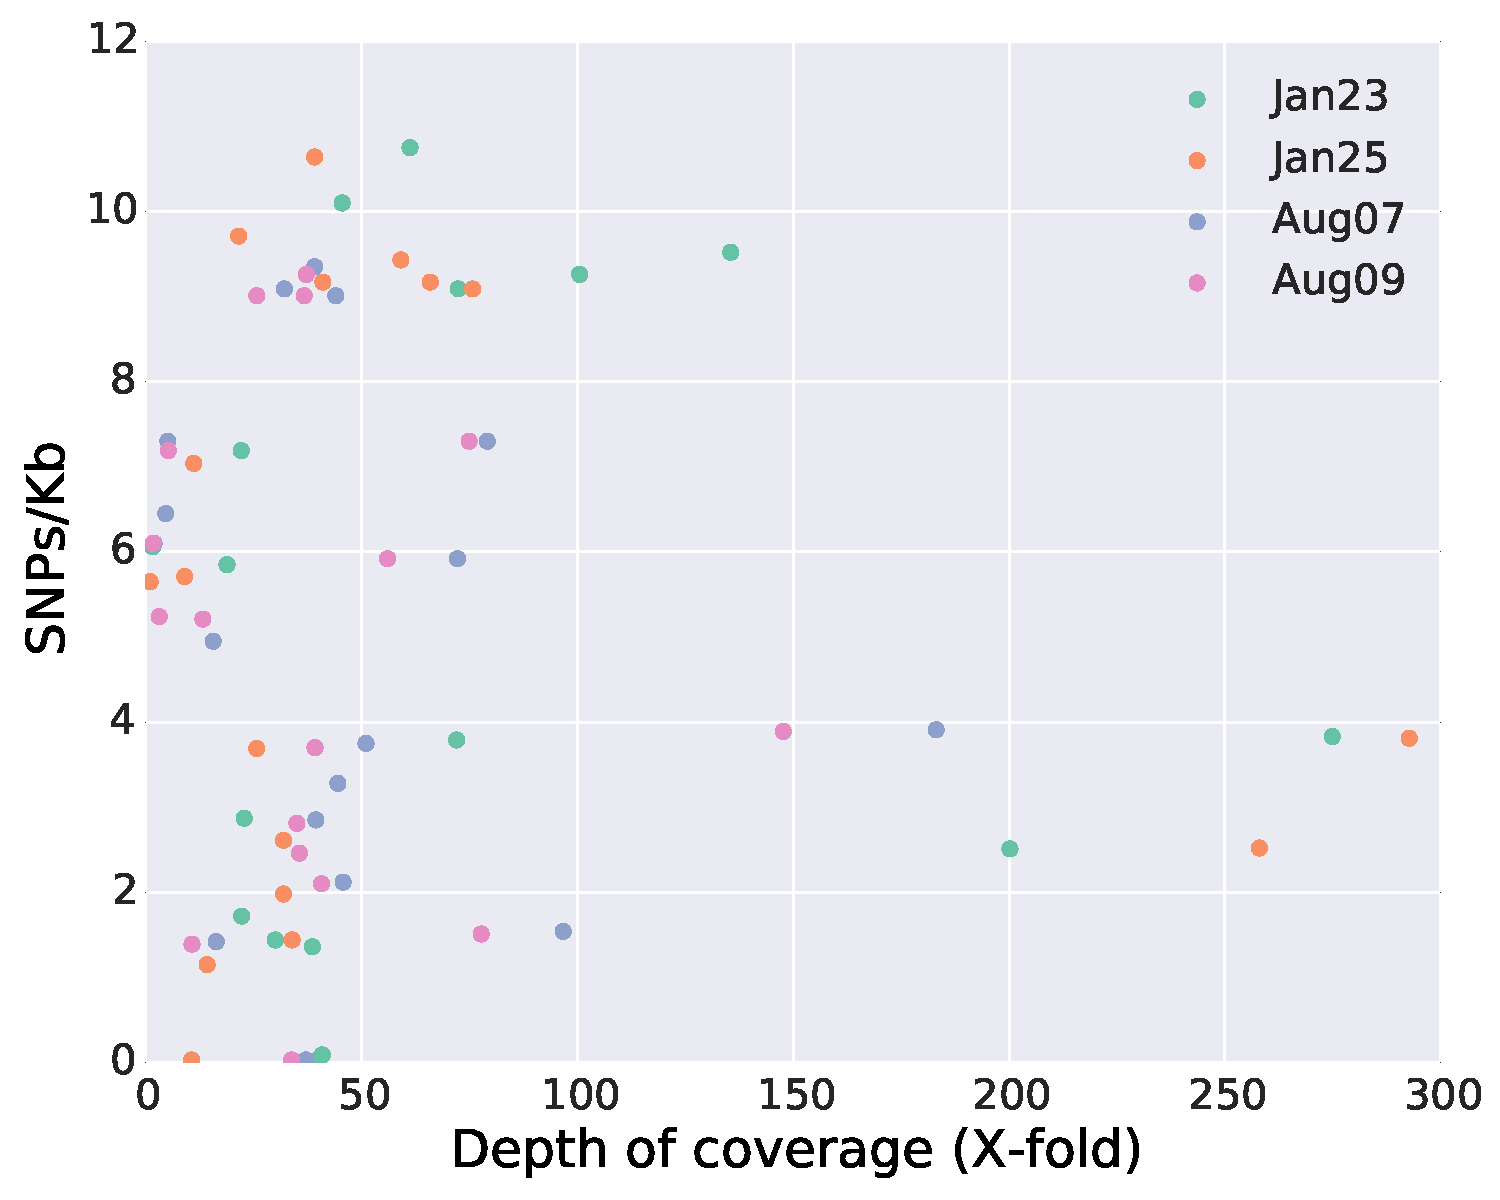
\includegraphics[width=0.7\textwidth,height=\textheight,keepaspectratio]{Chapter5/Figures/DepthCoverage_VS_SNPsKB.pdf}
  \caption{Scatterplot of depth of coverage versus SNPs/Kb for each of the reference genomes for the four libraries.}
  \label{SNPsCoverage}
\end{figure}

%
%%FIgures. Boxplot, SNPsKB
\begin{figure}[h]
  \centering
  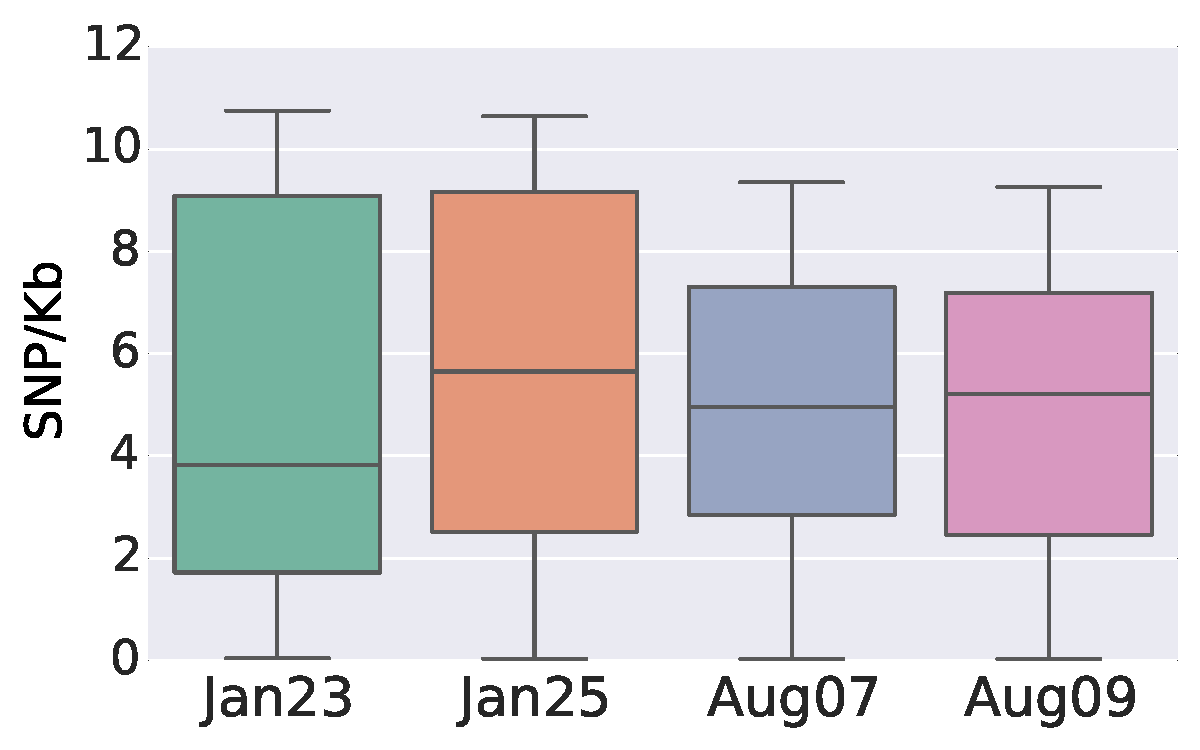
\includegraphics[width=0.6\textwidth,height=\textheight,keepaspectratio]{Chapter5/Figures/Boxplot_SNPsKB.pdf}
  \caption{Boxplot summarizing the number of SNPs/Kb for each genome, in each of the sequence libraries.}
  \label{BoxplotSNPsKB}
\end{figure}


%FIgures. SNP summary
\begin{figure}[h]
  \centering
  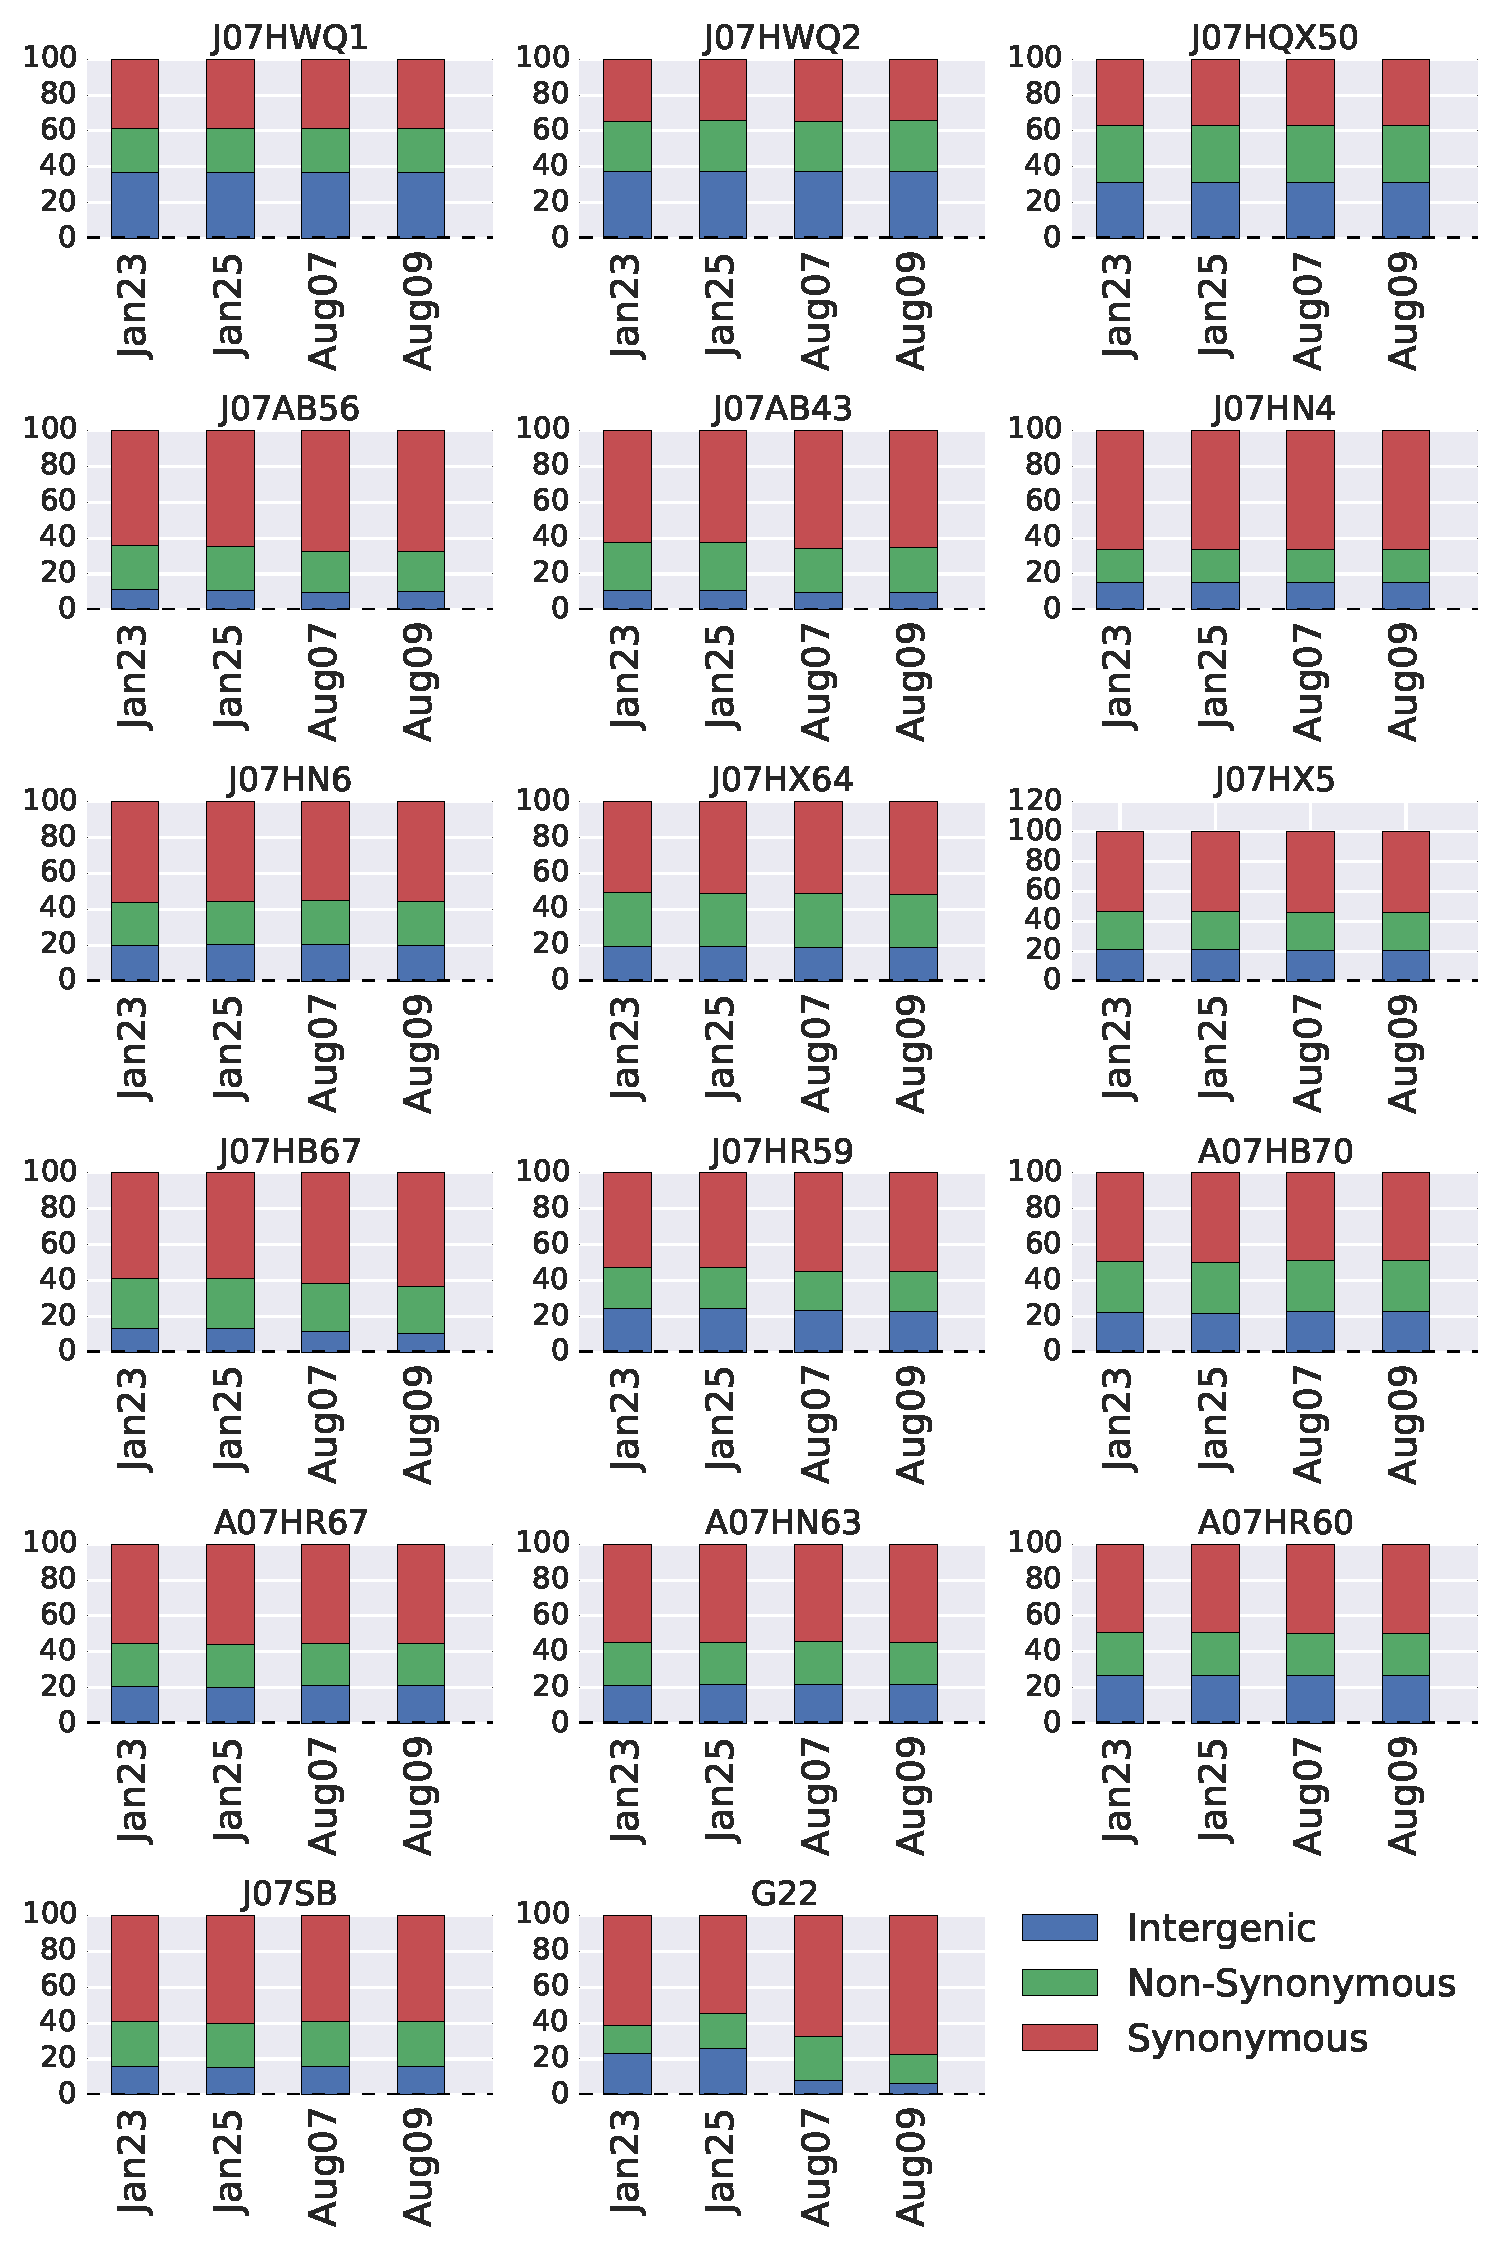
\includegraphics[width=\textwidth,height=0.8\textheight,keepaspectratio]{Chapter5/Figures/SNPsummary.pdf}
  \caption{Percentage of intergenic, non-synonymous and synonymous SNPs in each genome, for all the sequence libraries.}
  \label{SNPsummary}
\end{figure}

%Boxplot, type of SNPs
\begin{figure}[ht]
  \centering
  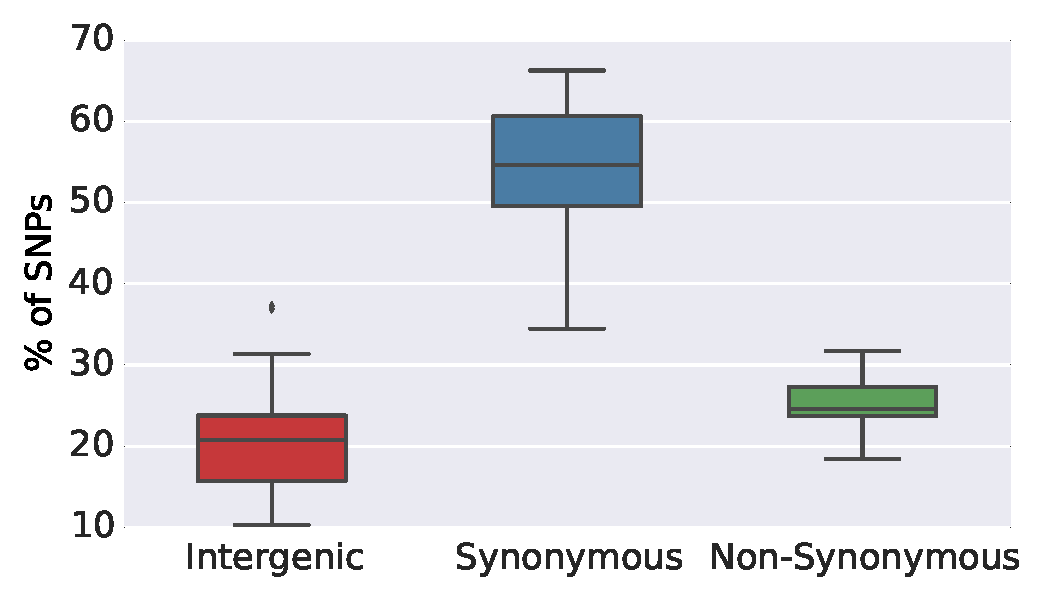
\includegraphics[width=0.7\textwidth,keepaspectratio]{Chapter5/Figures/BoxPlot_TypeofSNPs.pdf}
  \caption{Boxplot summarizing the distribution of type of SNPs (intergenic, synonynous, non-synonymous) for all the genomes and samples.}
  \label{BoxPlotSNP}
\end{figure}

%Figure VENN diagram January
\begin{figure}[!hbtp]
  \centering
  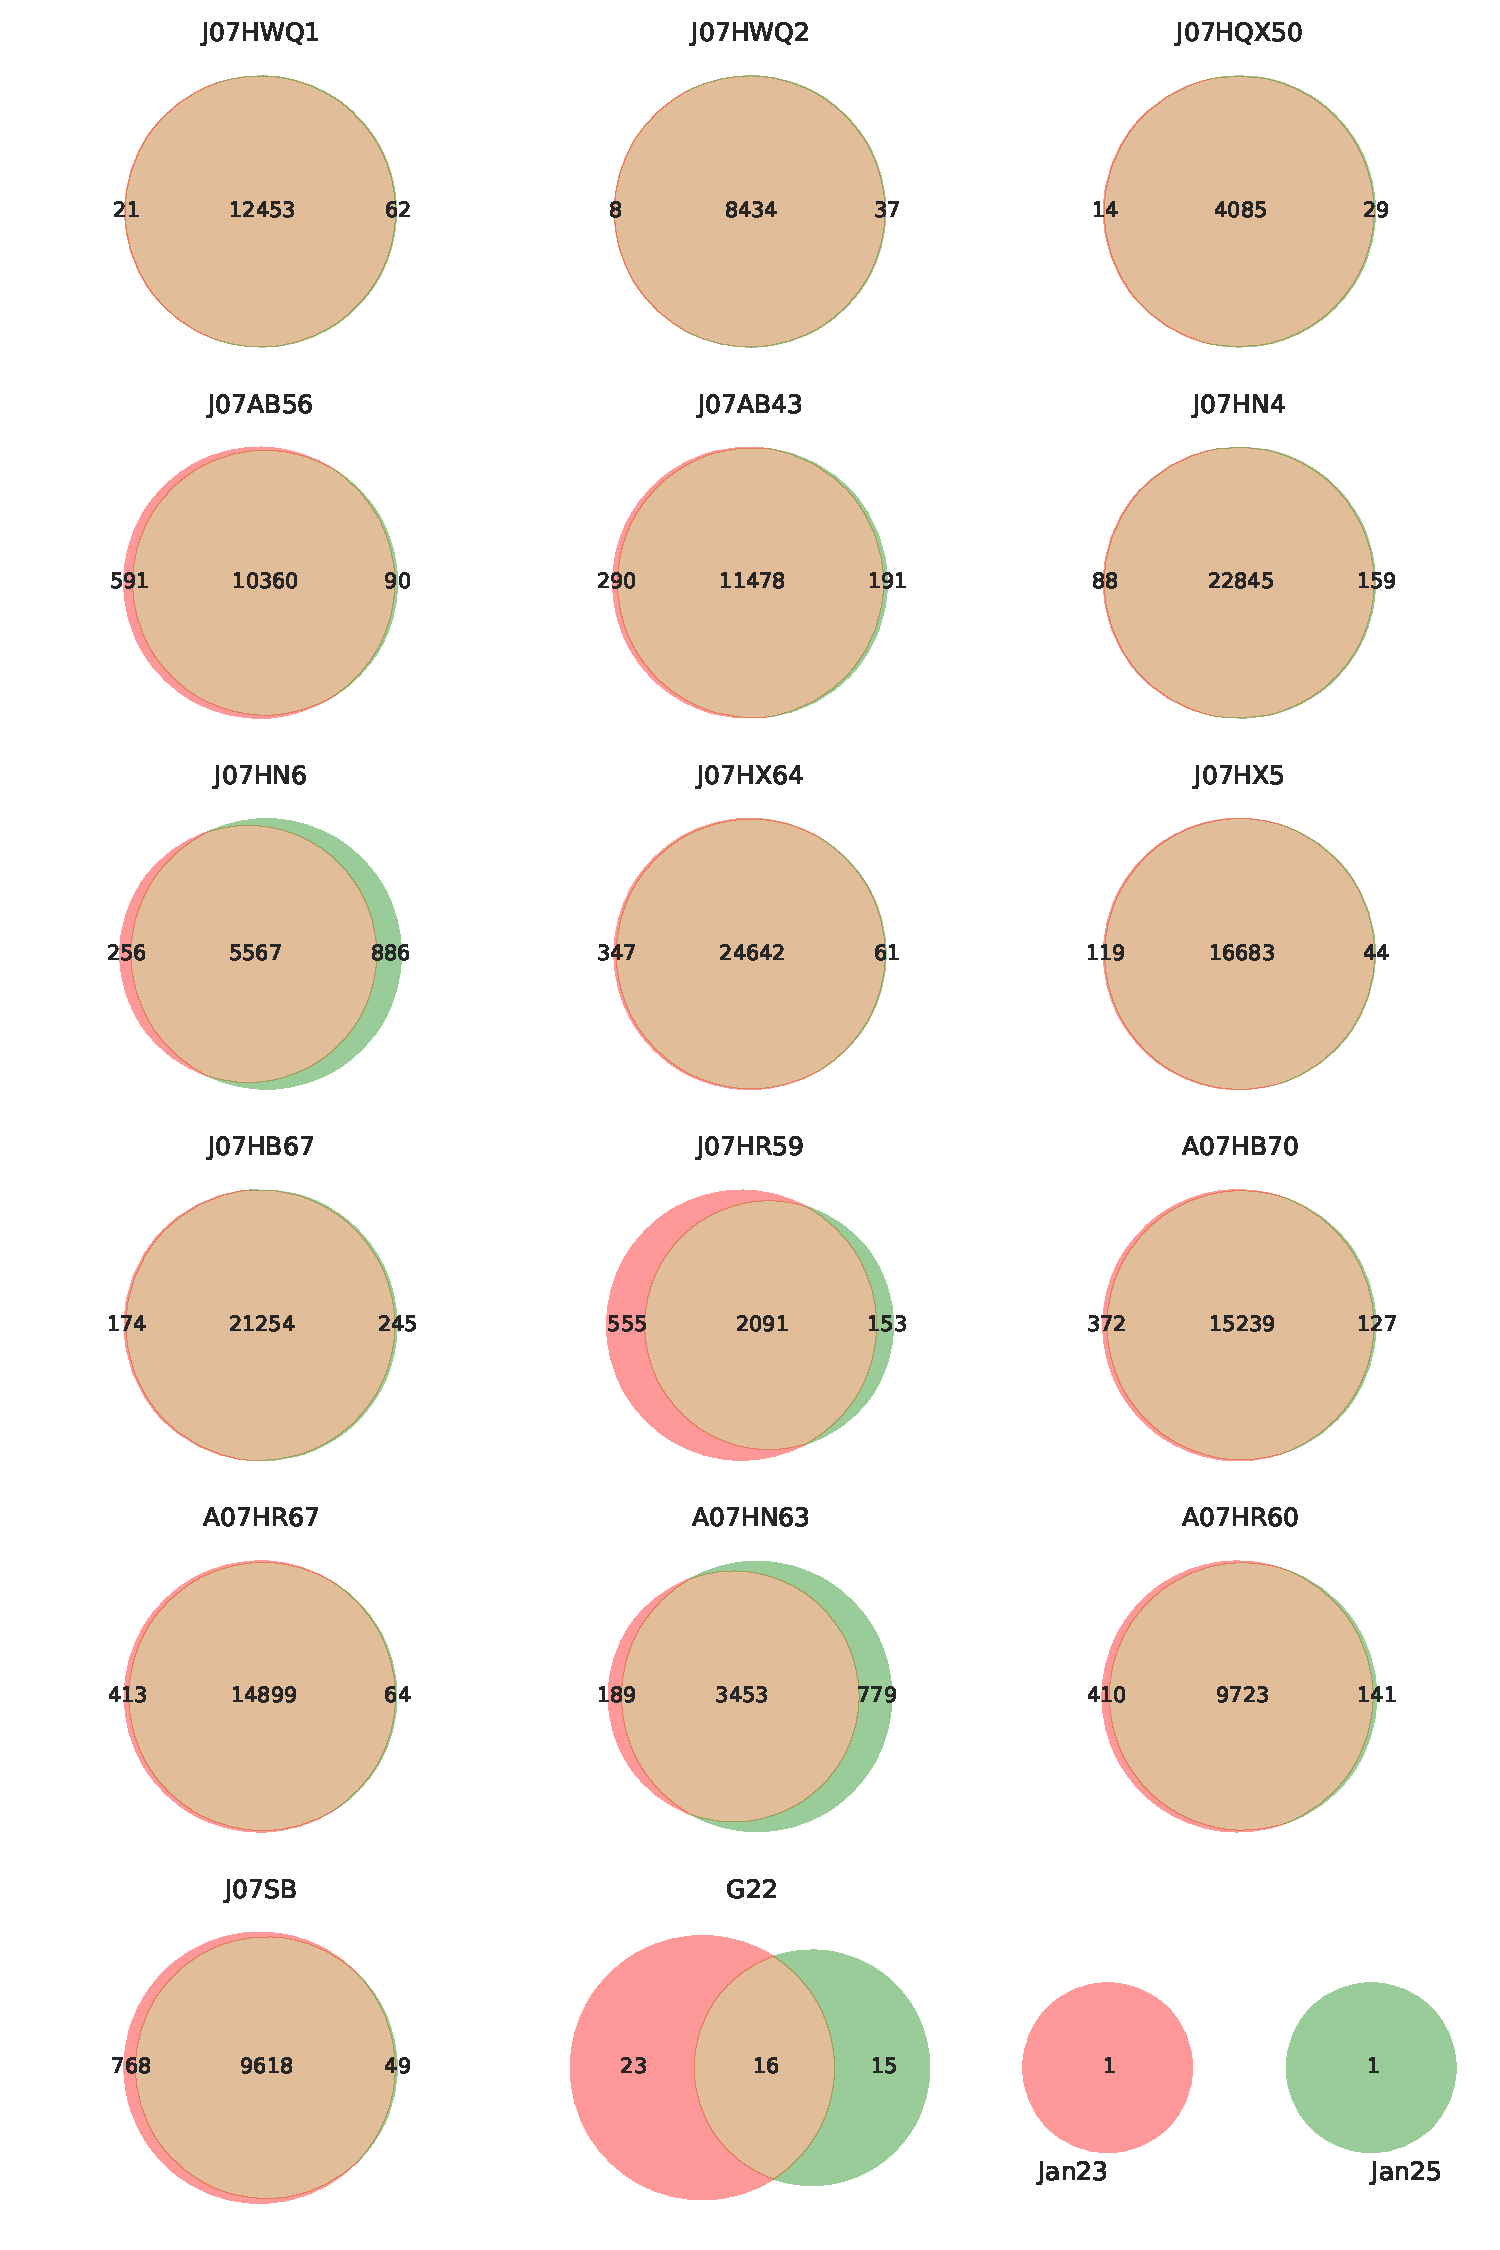
\includegraphics[width=\textwidth,height=0.9\textheight,keepaspectratio]{Chapter5/Figures/Venn_JanuarySNPs.pdf}
  \caption{Venn diagram comparing the SNPs found in the January 23 versus January 25 libraries.}
  \label{VennJan}
\end{figure}

%VENN diagram August
\begin{figure}[!hbtp]
  \centering
  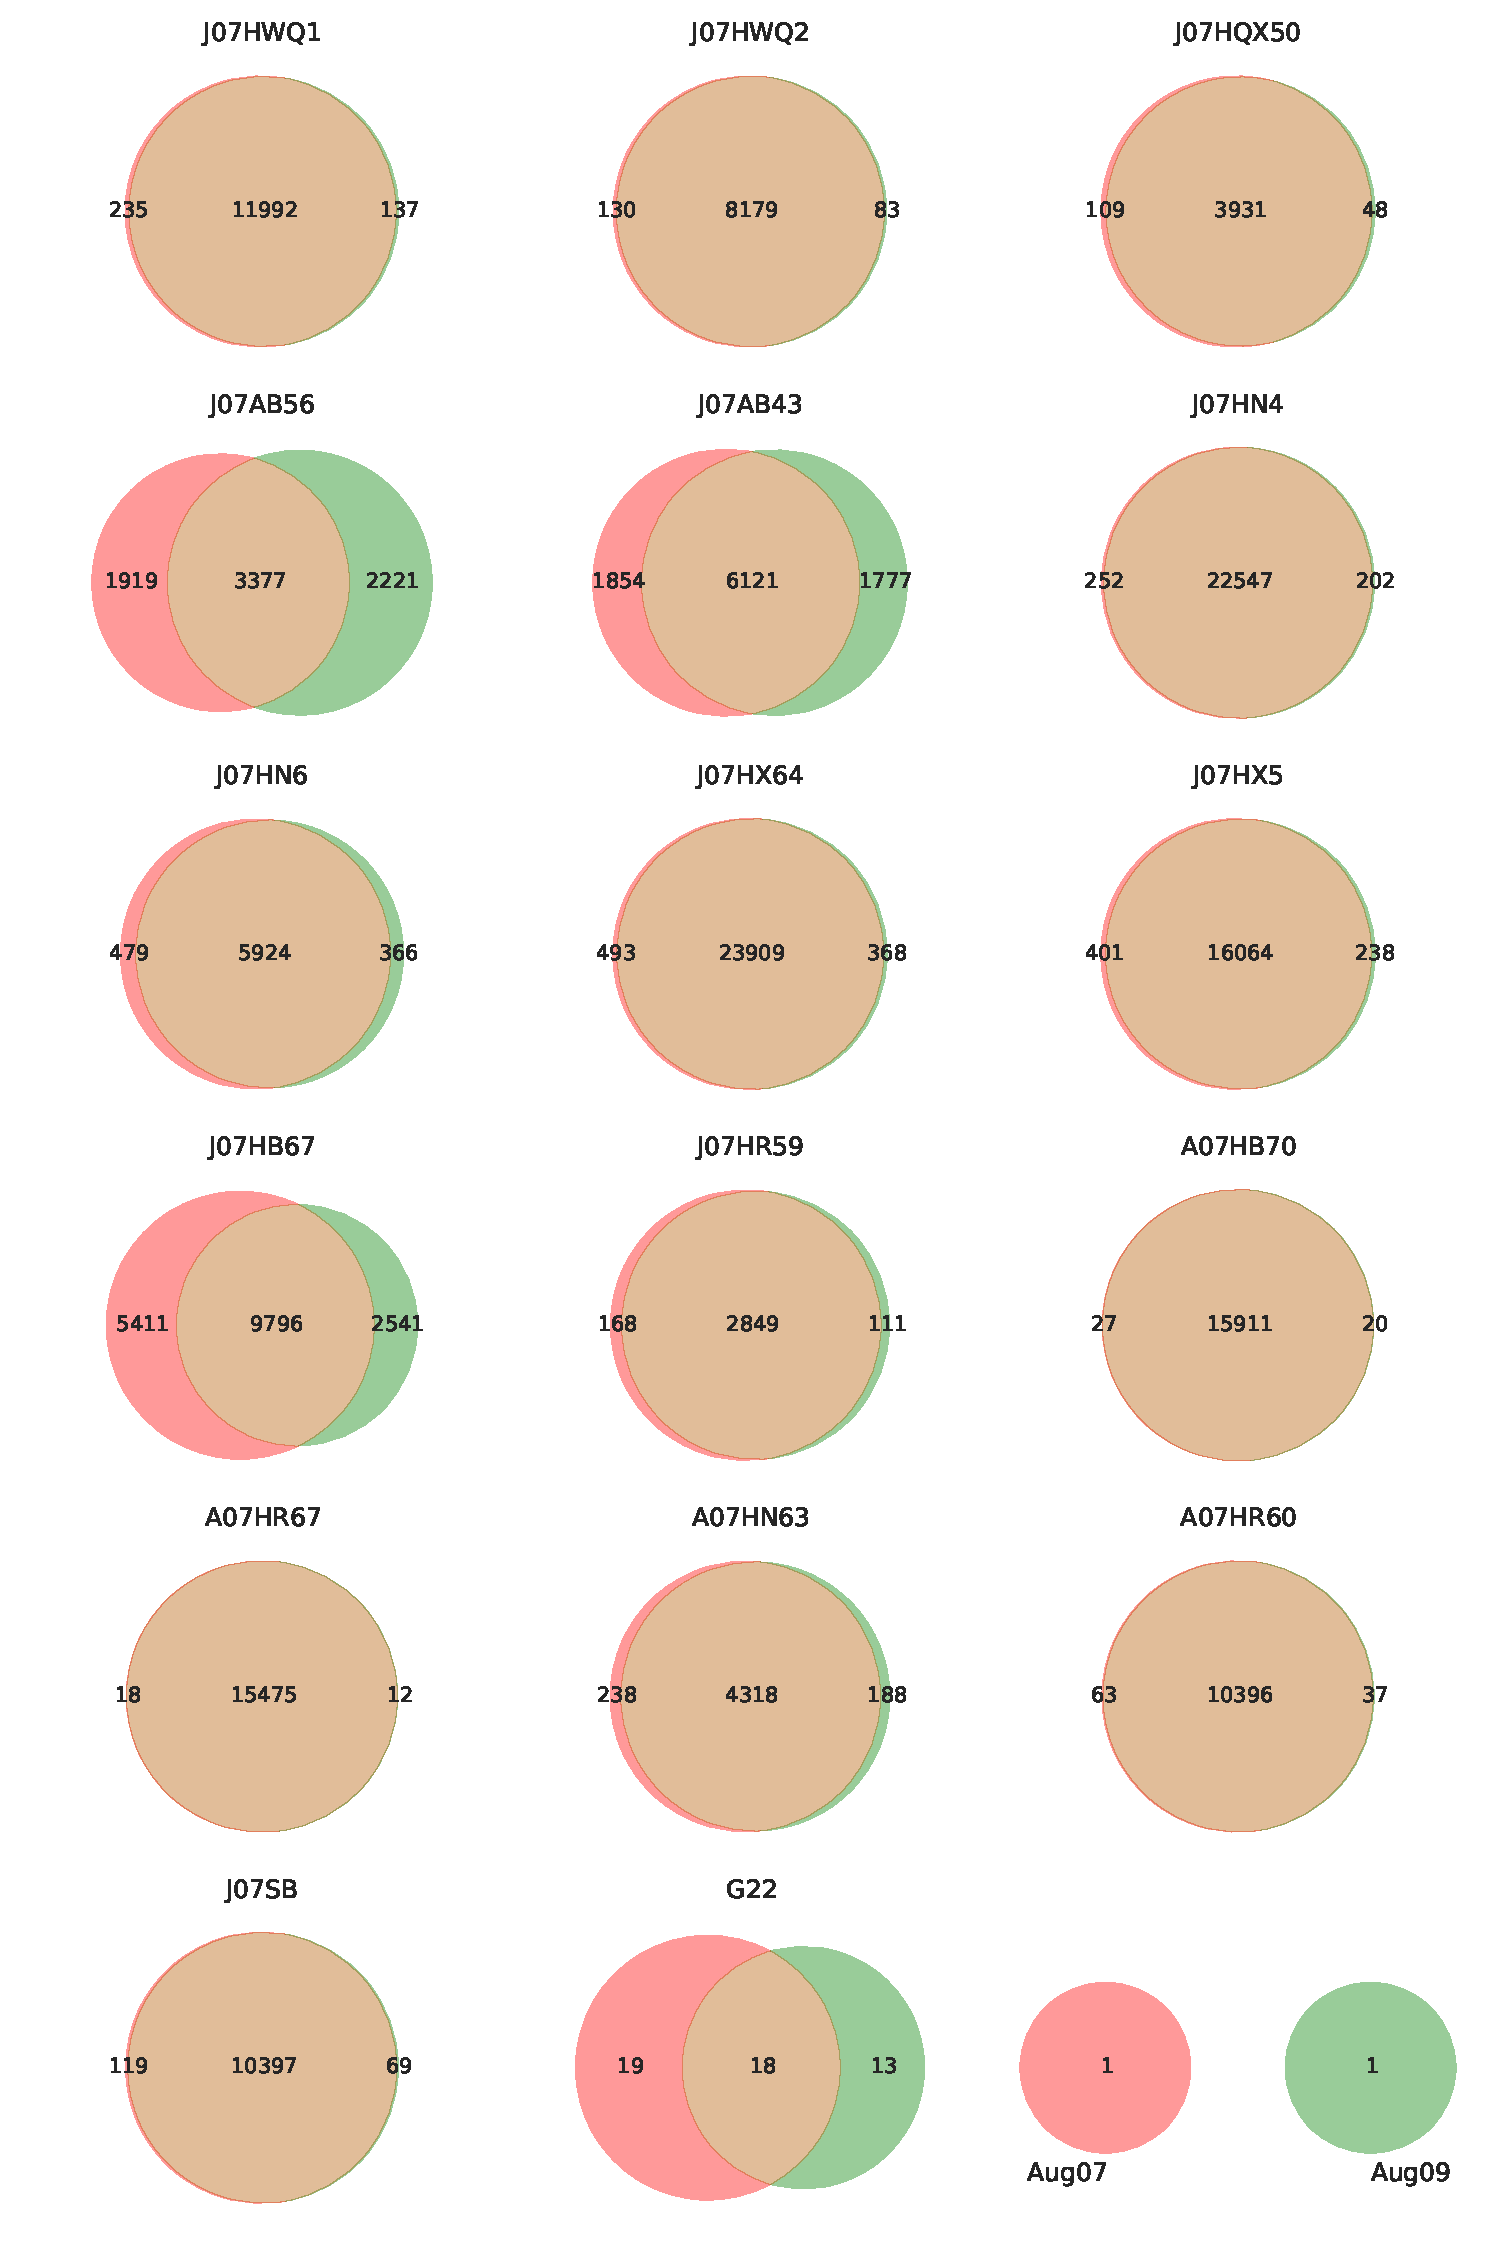
\includegraphics[width=\textwidth,height=0.9\textheight,keepaspectratio]{Chapter5/Figures/Venn_AugustSNPs.pdf}
  \caption{Venn diagram comparing the SNPs found in the August 7 versus August 9 libraries.}
  \label{VennAug}
\end{figure}

%VENN digram both
\begin{figure}[!hbtp]
  \centering
  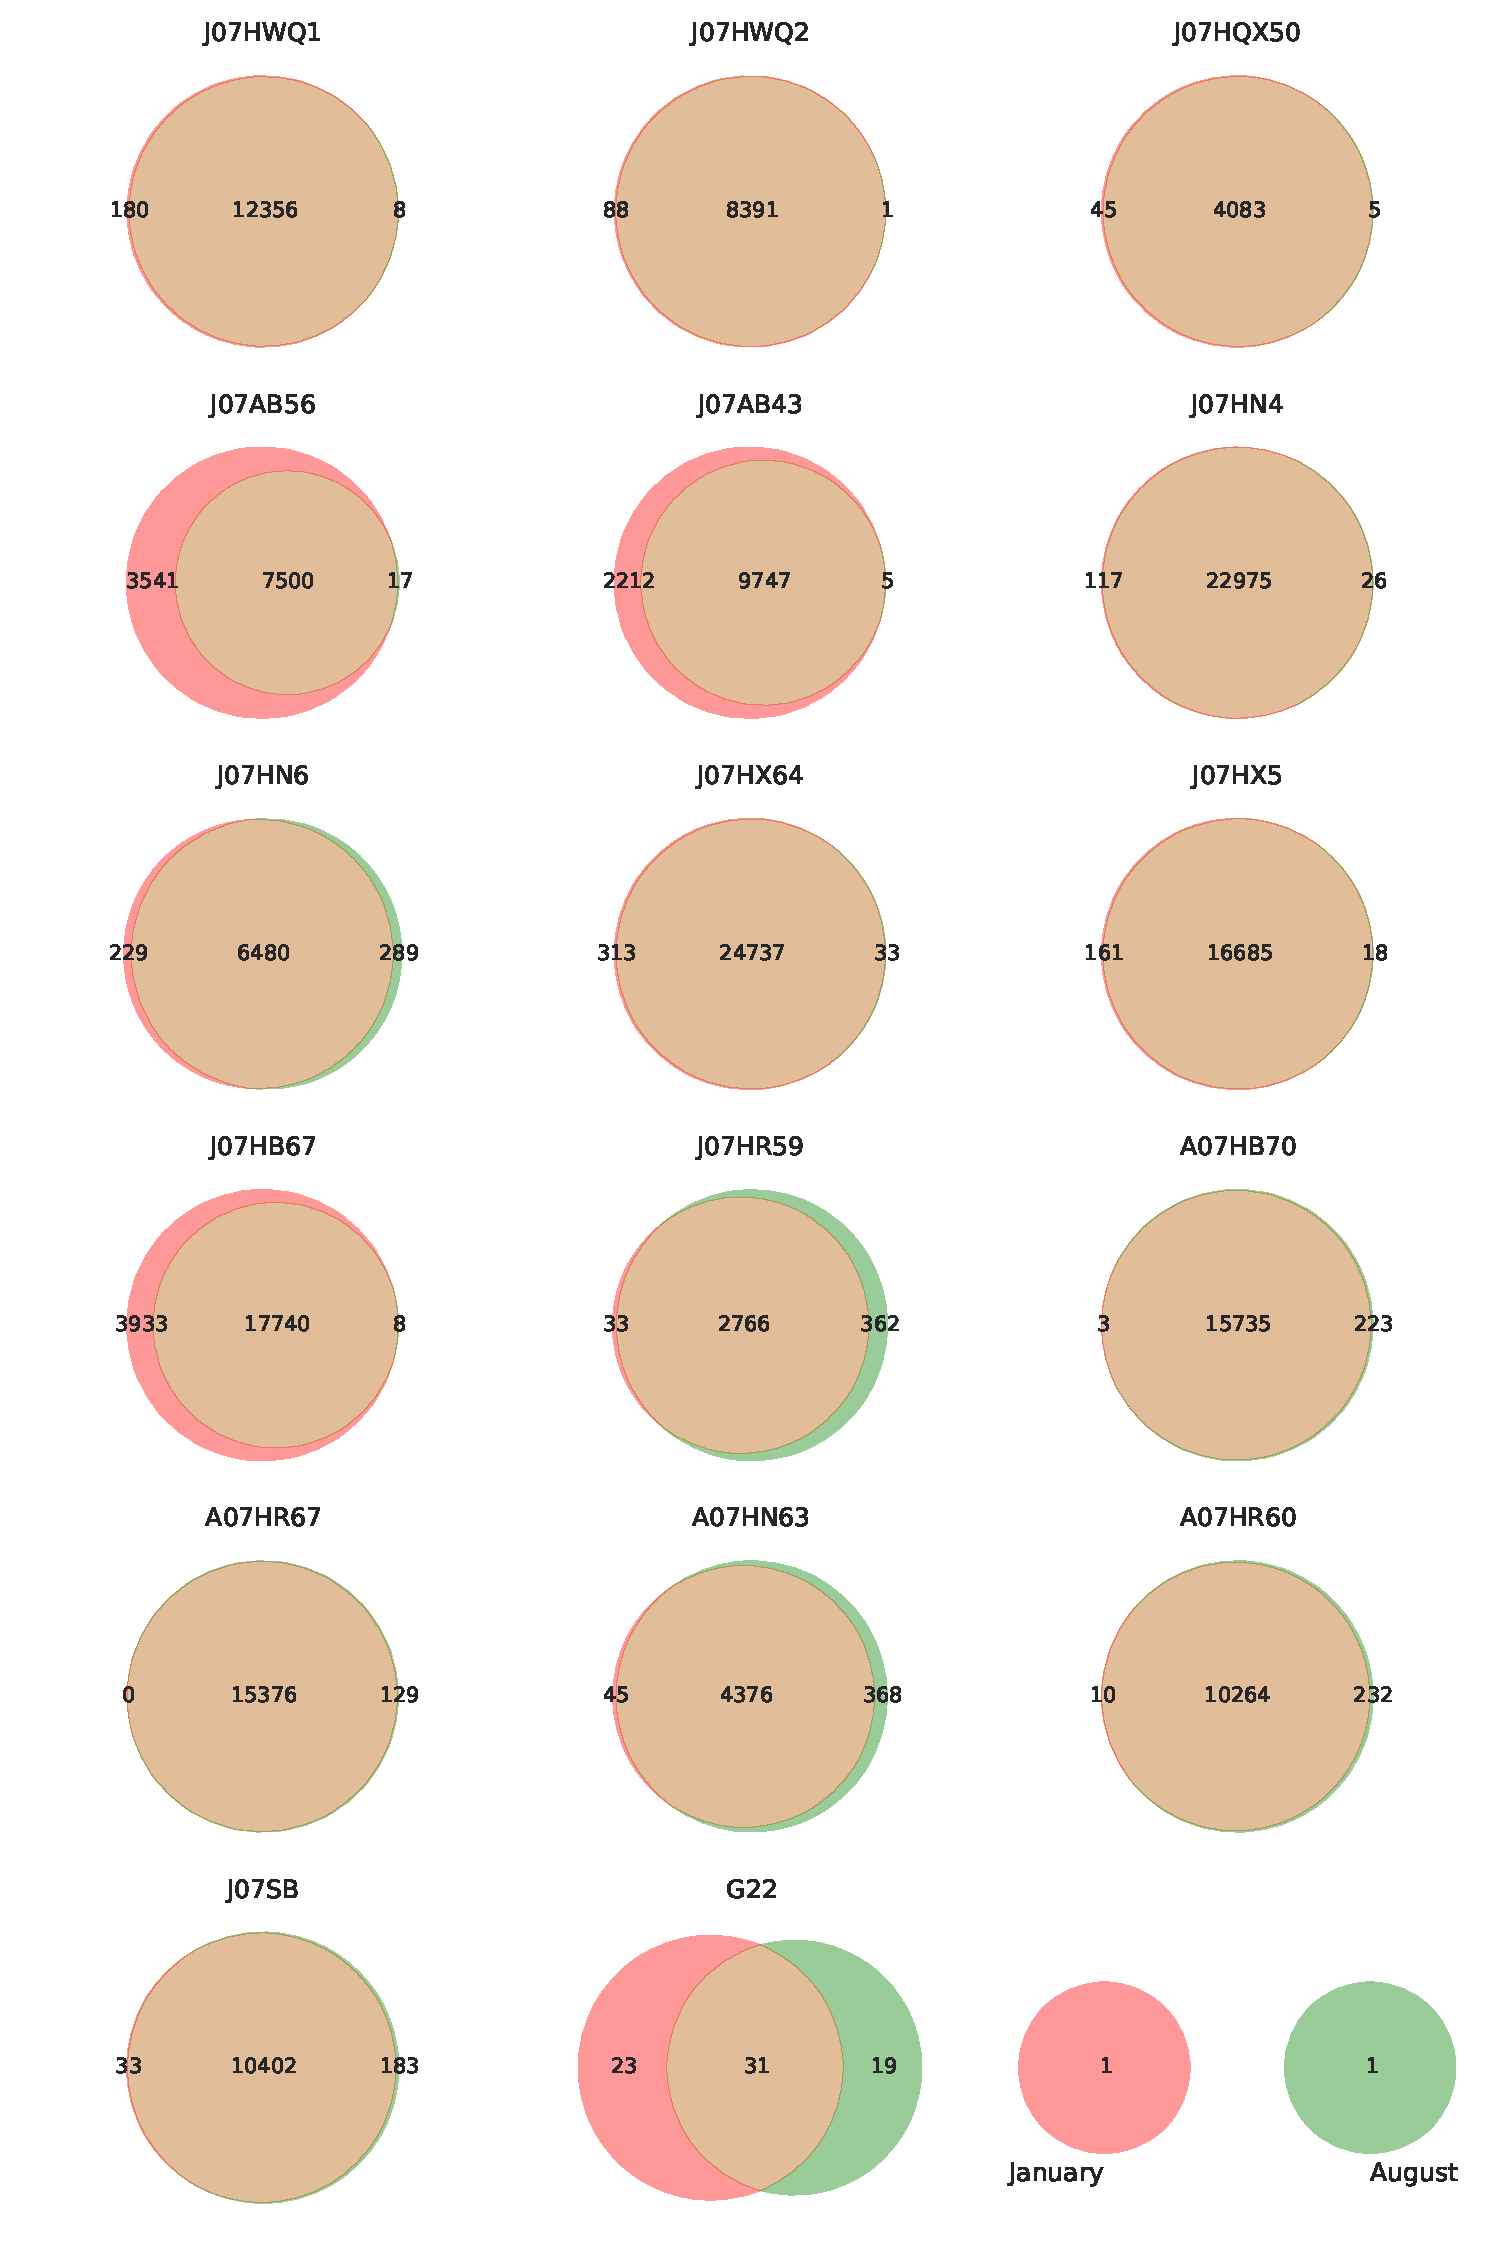
\includegraphics[width=\textwidth,height=0.9\textheight,keepaspectratio]{Chapter5/Figures/Venn_JanAugSNPs.pdf}
  \caption{Venn diagram comparing the SNPs found in the January versus the August libraries}
  \label{VennBoth}
\end{figure}


%%%%%%%%%%%%%%%%%%%%%%%
\clearpage
\subsection{Genes under positive selection}

The results from the variant analyses, allows to evaluate the role that natural selection is playing in the evolution of individual genes within the population. One approach to do this, is to look at the ratio between non-synonymous to synonymous substitution on each individual genes. This is defined as the dN/dS ratio \cite{McDonald:1991hj}, which compares genes between individual species. Similarly, the pN/pS ratio compares this effect at the population level, which is the case in here, where we do not have individual isolates that are being under study, but a complex sample \cite{Egea:2008jo,Schloissnig:2012hx}. Using the pN/pS ratio, we can identify genes that under the effects of positive selection (pN/pS $>$ 1), where natural selection is favoring diversification at the amino acid level \cite{Hurst:2002ht}. On the other extreme, purifying selection (pN/pS $<$ 1) occurs when fewer amino acid changes occur that the one expected by chance \cite{Hurst:2002ht}.

There are multiple methods for detecting molecular adaptation based on pN/pS ratios \cite{Yang:2000hh}. Because short reads are being used to identify polymorphisms in the genomes, is not possible to link multiple polymorphisms. This makes statistical approaches, such as maximum likelihood methods and bayesian methods, difficult to implement for our data \cite{Yang:2000hh}. Instead, a pairwise method was used, quantifying the polymorphisms site by site, using a strategy based on previous work by Tai \textit{et al.} \cite{Tai:2011jo} (Figure \ref{MappingStrategy}). 

\subsubsection{Average pN/pS values for each genome}

First, the average pN/pS values were calculated for each of genomes, to determine overall patterns of selection between samples. Figure \ref{Genome_comp_pNpS} shows a comparison of the average pN/pS value for each genome, between the months of January and August. Besides the extreme value of G22, no large differences are observed between the two months. This suggest that the overall values of pN/pS for the genes are similar between the two sampling dates.


\subsubsection{pN/pS values and uniquely selected genes}

The pN/pS values were calculated for all the coding regions in each of the reference genomes. To facilite the comparisons, the analysis was limited to the comparisons between the January and August datasets, merging each individual time point within the same sampling month. An overview of each genome (Appendix \ref{Appendix_pNpS}), shows that visually it does not appear to be hotspots of selection across the genomes. For example, in the genomes of J07HWQ1 (Figure \ref{example_J07HWQ1_pNpS}) and J07HWQ (Figure \ref{example_J07HWQ2_pNpS}), no striking differences between January and August were observed. Also, the genes under selection are located sparsely along the genome.

Comparing more in detail January versus August, for each reference genome, the results (Table \ref{PSgenes}) indicate that in both samples the number of genes under positive selection (pN/pS $>$ 1) is similar within each of the reference genomes. Comparing across the genomes, we can see that the percentage of genes under selection in each of the genomes, varies between ~1.5\% up to 7\% (without considering G22). This is similar to values observed in comparisons for isolate genomes of \textit{Salinibacter} \cite{PeNtildeA:2010ie}, as well in other similar metagenomic studies in \textit{Synechococcus} populations \cite{Tai:2011jo}. A very interesting result, that is similar to what was observed by just looking at the number of shared SNPs between sampling months, is that for several of the genomes, the same genes are under selection in January versus August. Although more formal population analysis needs to be done to be sure about this, this strongly suggests that for some organisms like \textit{Haloquadratum} (J07HWQ1, J07HWQ2 and J07HQX50) and \textit{Halonotius} (J07HN4 and J07HN6), among others, the strain variation present in January is similar to the one in August \cite{Vos:2011ux}. For organisms like \textit{Nanohaloarchaea} (J07AB56 and J07AB43), the differences suggest the opposite, that there are difference in the strain diversity present in January versus August. By focusing in the genes that are different between sampling months, we can look more in detail at this variation, providing examples of some of the encountered differences.

In the case of J07HWQ1, the single gene that is unique in the August sample, codifies for a predicted cobalamin biosynthesis protein (according to the COG prediction), and has a von Willebrand factor, type A domain. This protein family has a wide range of functions, and in the case of the J07HWQ1 genome is located next to a predicted ATPase associated diverse cellular activities. The annotation of both of this protein does not suggest a particular role for the positive selected gene, as it may fall into a wide variety of roles, including DNA repair, transcription, ribosomal and membrane transport, cell adhesion, among other roles \cite{Whittaker:2002ug,Makarova:2010bi}.

For J07HWQ2, the gene that is under positive selection in January, codifies for an hypothetical protein that is rich in serine residues. No function is associated with this sequence, but recent evidence from studies in Dictyostelid amoebae, suggest that this domains are frequently present and functional in eukaryote genomes \cite{Tian:2013jv}. In the August sample, the gene under selection codifies for an amino acid transporter.

The other example that will be explored here, is the other extreme, the genomes of the \textit{Nanohaloarchaea} (J07AB56 and J07AB43), where we observe differences in the genes that are under positive selection. In J07AB56, the January genes codify for hypothetical proteins, transcriptional regulators, chaperones, among other functions. Interestingly, a large number of proteins related to transmembrane functions was found, including transporters and transmembrane proteins. In contrast, the functions enriched in August, tend to be more hypothetical proteins and some proteins involved in beta-lactamase functions. 

For J07AB43, the differences are hard to pinpoint to specific functional roles, as in both cases over 70\% of the functions are annotated as hypothetical proteins. An interesting protein that is under selection in the January sample encodes for a photolyase, involved in light-drive DNA repair \cite{Weber:2005fk}. This could be related to the different environmental conditions, in particular light intensity and temperature, between the two sampling dates.

\subsubsection{Differences between pN/pS values between sampling dates}

Even when for some of the analyzed genomes, the same genes appeared to be under positive selection comparing the January and August samples, even in genes that are under selection in both samples, differences in their pN/pS values (Figure \ref{Gene_pN_pS}), can be observed. In some of the organisms like the \textit{Haloquadratum} genomes, only a few genes show different values in one of the samples. On the other hand, in the \textit{Nanohaloarchaea}, there is a broad dispersion of the values, indicating differences in the nucleotide diversity of some of these genes, which could be translated into different number of strains for these organisms. This also supports the idea that the J07AB43 populations that are present in the January sample, are different from the one present in the August sample \cite{Vos:2011ux}. A similar  pattern is observed in the J07HB67 genome, and to a lower degree in the A07HN63 genome.


\subsubsection{pN/pS values and functional classification}

One of the limitations of the analysis of pN/pS values, is that unless experimental evidence is available for some of the candidate genes, in most of the cases the associated functions tend to be hypothetical proteins \cite{Tai:2011jo}. At the same time, this is one of the powerful things in the analysis, as it can provide candidates for further experimental studies, at least where isolates are available \cite{Fricke:2011gy}.

To narrow some of the functions that could be under selection, the COG (cluster of orthologous groups) functional categories were used. All the genes that had a COG number assigned were analyzed, and COG categories that could be enriched in genes under selection were evaluated, by comparing them with the classification of the complete genome (Appendix \ref{Appendix_COGselection}). These results were validated by calculating the odds ratio (the difference between the categories with genes under selection, versus the rest of the annotated cogs for the genome), with a one-tailed Fisher exact test (pvalue $<$ 0.05). This analysis provided some functional information on some of the genomes and the genes that are under selection. 

For example, in the case of J07HQX50, the cell wall/membrane/envelope biogenesis category, has three genes that are under positive selection. Looking at these genes in more detail, all of them are involved in lipopolysaccharide synthesis, two of them with functions related to the surface layer modification, and the other as a sugar transferase. Considering that these genes are under selection both in January and August, these could suggest that J07HQX50 is under some type of selective pressure to modify its membrane composition, which could be due to multiple factors, including phage predation \cite{RodriguezValera:2009cr}.

Another interesting example can be found on J07AB56 (Table \ref{January_COG_Selection_J07AB56}), where in the January sample, the cell motility category is enriched in genes under positive selection. Looking in detail there are four genes in these group, all of them encoding secretion system proteins. Three of them encode for VirB11 components of the type IV secretory pathway, which could play a role in DNA uptake or protein secretion \cite{Chandran:2009fg}. In the August sample, a different category is enriched, intracellular trafficking, secretion and vesicular transport, but a detailed look of the genes, shows that most of them encode for type IV secretory systems, or protein export component, suggesting a similar role as in the January case, where the genes involved in protein secretion are under positive selection. It has been observed in Bacteria that secreted proteins have rapid evolution rates \cite{Nogueira:2012gv}, and some of these proteins could be involved with interaction with the outside environment, as they could be attached to the cell wall, and include functions such as protection against grazing \cite{Matz:2005ik} and competitions against other microbial groups \cite{Kirkup:2004hj}.


%Figure Mapping
\begin{figure}[!hbtp]
  \centering
  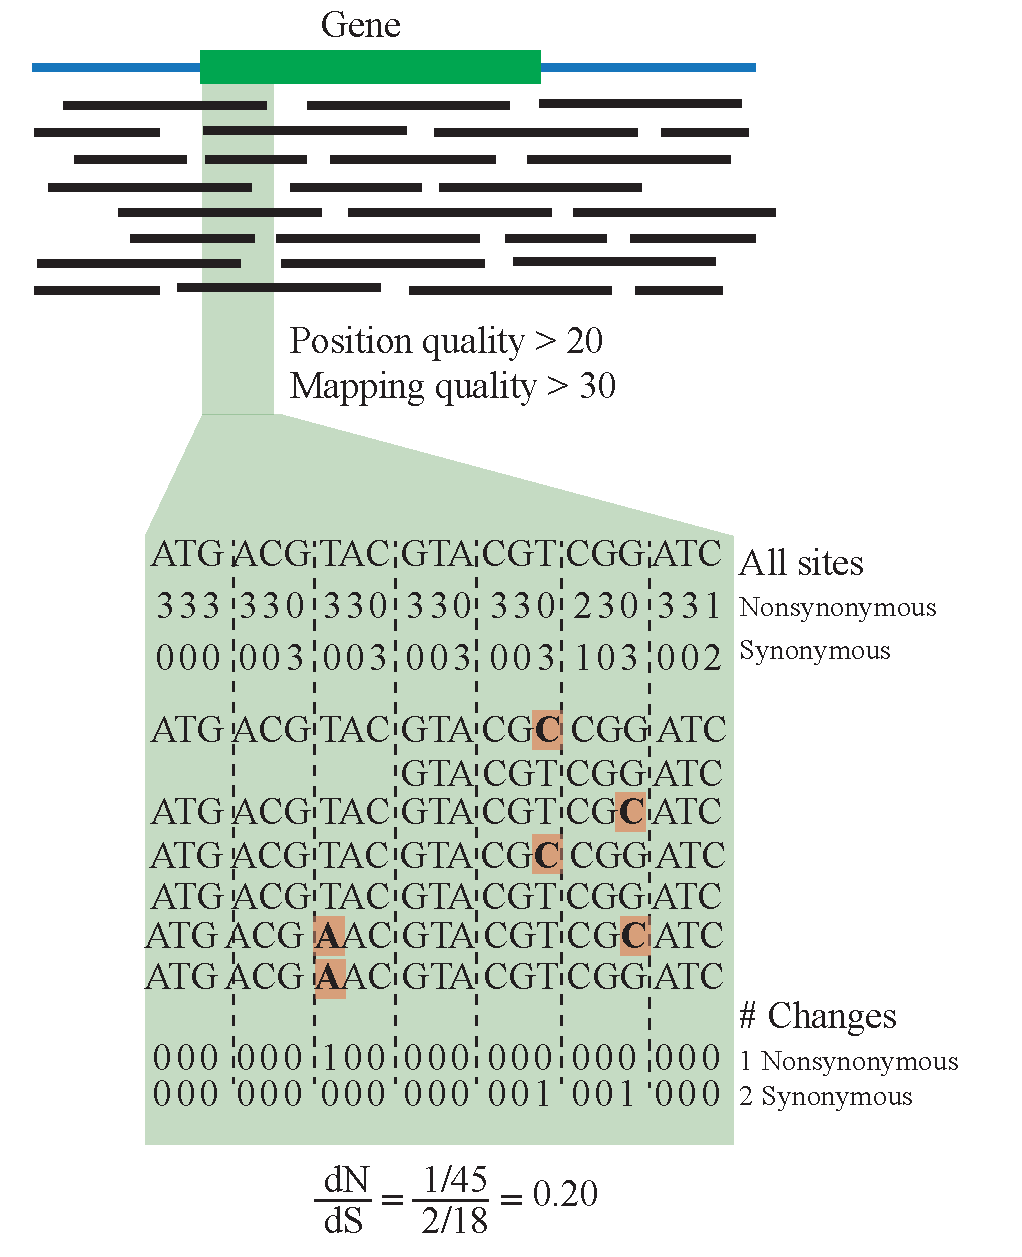
\includegraphics[width=0.7\textwidth]{Chapter5/Figures/MappingStrategy.pdf}
  \caption{Overview of the strategy used to quantify the SNPs differences on each gene, and calculate the ratio of non-synonymous to synonymous substitutions (pN/pS) on each of the reference genome. Figure based on \cite{Tai:2011jo}.}
  \label{MappingStrategy}
\end{figure}

%Table Genes positive selection
\begin{table}[hbt]
  \caption{Count of Genes under positive selection (pN/pS $>$ 1). Data where pS/pS = 0/0 or pS = 0, was not included.}
  \begin{tabularx}{\textwidth}{L{2.2cm}R{2cm}R{3cm}R{3.2cm}R{2cm}}
  \hline
    \textbf{Genome} & \textbf{CDS} & \textbf{January} & \textbf{August} & \textbf{Unique (Jan/Aug)} \\
    \hline
     \textit{J07HWQ1} & 3,584 & 61 (1.7) & 62 (1.7) & 0/1 \\
     \textit{J07HWQ2} & 3,856 & 46 (1.2) & 46 (1.19) & 1/1 \\
     \textit{J07HQX50} & 2,872 & 19 (0.7) & 19 (0.7) & 0/0 \\
     \textit{J07AB56} & 1,411 & 96 (6.8) & 79 (5.6) & 37/20 \\
     \textit{J07AB43} & 1,678 & 96 (5.7) & 87 (5.2) & 25/16 \\
     \textit{J07HN4} & 3,230 & 198 (6.1) & 196 (6.1) & 3/1\\
     \textit{J07HN6} & 2,914 & 59 (2.1) & 64 (2.2) & 3/8 \\
     \textit{J07HX64} & 3049 & 191 (6.2) & 189 (6.2) & 3/1 \\
     \textit{J07HX5} & 2,139 & 137 (6.4) & 137 (6.4) & 1/1 \\
     \textit{J07HB67} & 2,847 & 196 (6.8) & 168 (5.9) & 54/26 \\
     \textit{J07HR59} & 1,841 & 27 (1.4) & 33 (1.8) & 0/6 \\
     \textit{A07HB70} & 2,514 & 154 (6.1) & 156 (6.2) & 1/3 \\
     \textit{A07HR67} & 2,891 & 167 (5.8) & 171 (5.9) & 0/4 \\
     \textit{A07HN63} & 2,507 & 42 (1.7) & 50 (2.0) & 4/12 \\
     \textit{A07HR60} & 2,861 & 83 (2.9) & 87 (3.1) & 2/6 \\
     \textit{G22} & 3,525 & 0 (0) & 0 (0) & 1/1 \\
     \textit{J07SB} & 1,641 & 91 (5.6) & 91 (5.5) & 2/2\\     
  \end{tabularx}
  \label{PSgenes}
\end{table}

%Figure COG pNpS average
\begin{figure}[]
  \centering
  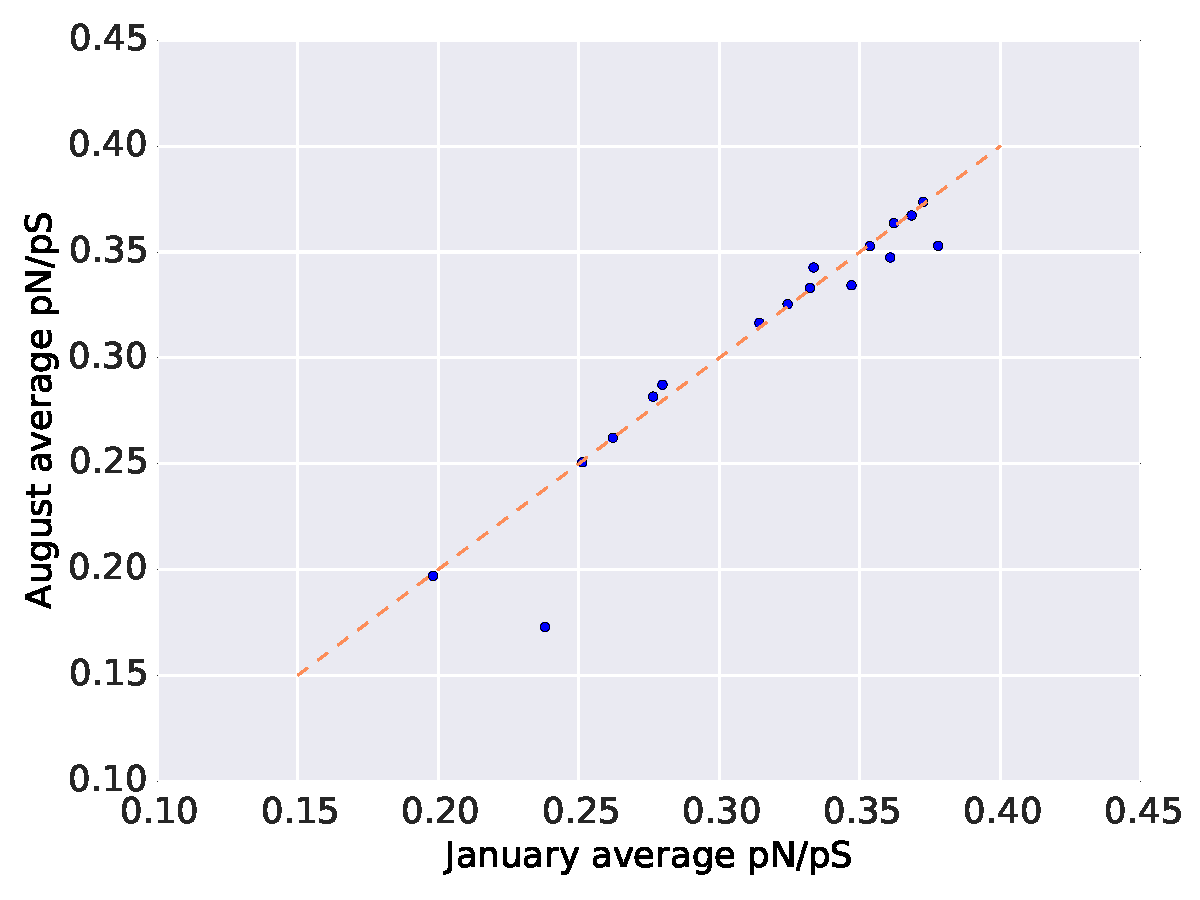
\includegraphics[width=0.75\textwidth,height=\textheight,keepaspectratio]{Chapter5/Figures/Scatter_Genomes_pNpS.pdf}
  \caption{Scatterplot of average pN/pS ratios in January versus August, for each of the reference genomes used in the analysis. The extreme value in the right bottom of the plot, corresponds to G22.}
  \label{Genome_comp_pNpS}
\end{figure}


%Figure COG pNpS average
\begin{figure}[]
  \centering
  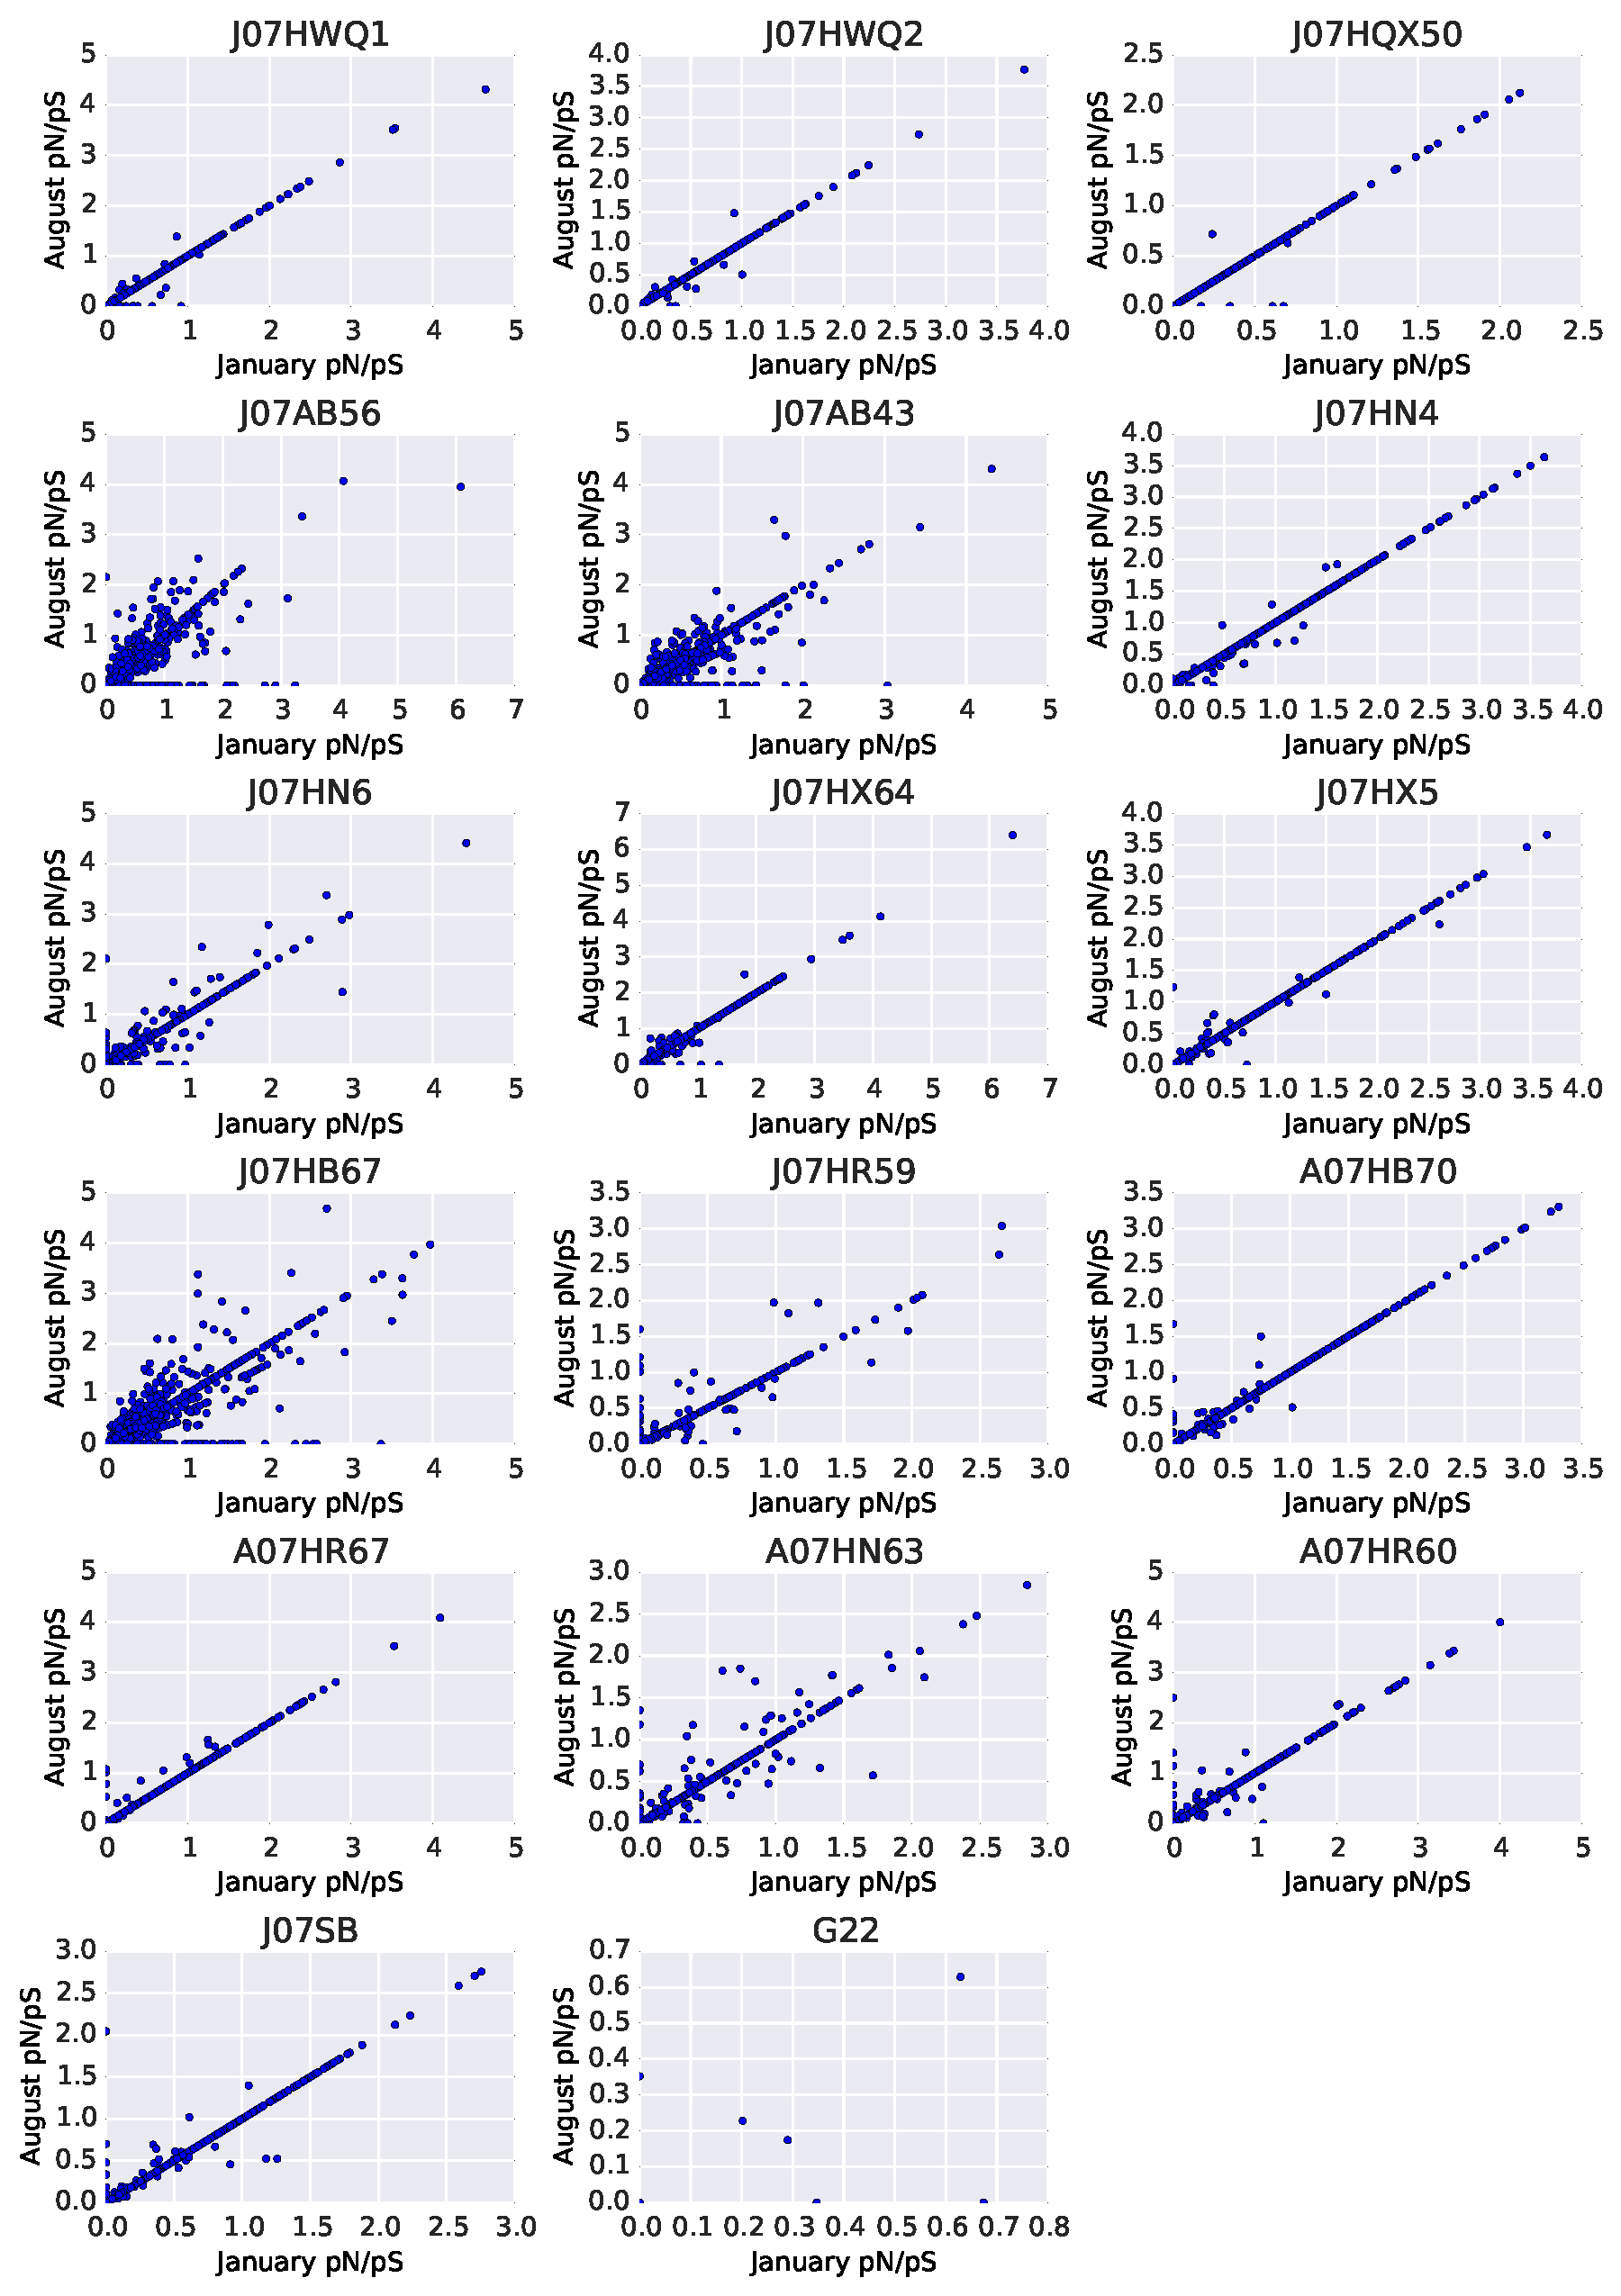
\includegraphics[width=\textwidth,height=0.8\textheight,keepaspectratio]{Chapter5/Figures/Gene_pN_pS.pdf}
  \caption{Scatterplot of the pN/pS values for each of the reference genomes, comparing the pN/pS values in January versus August.}
  \label{Gene_pN_pS}
\end{figure}

%Figures pn/ps along genome
\begin{figure}[p]
  \centering
  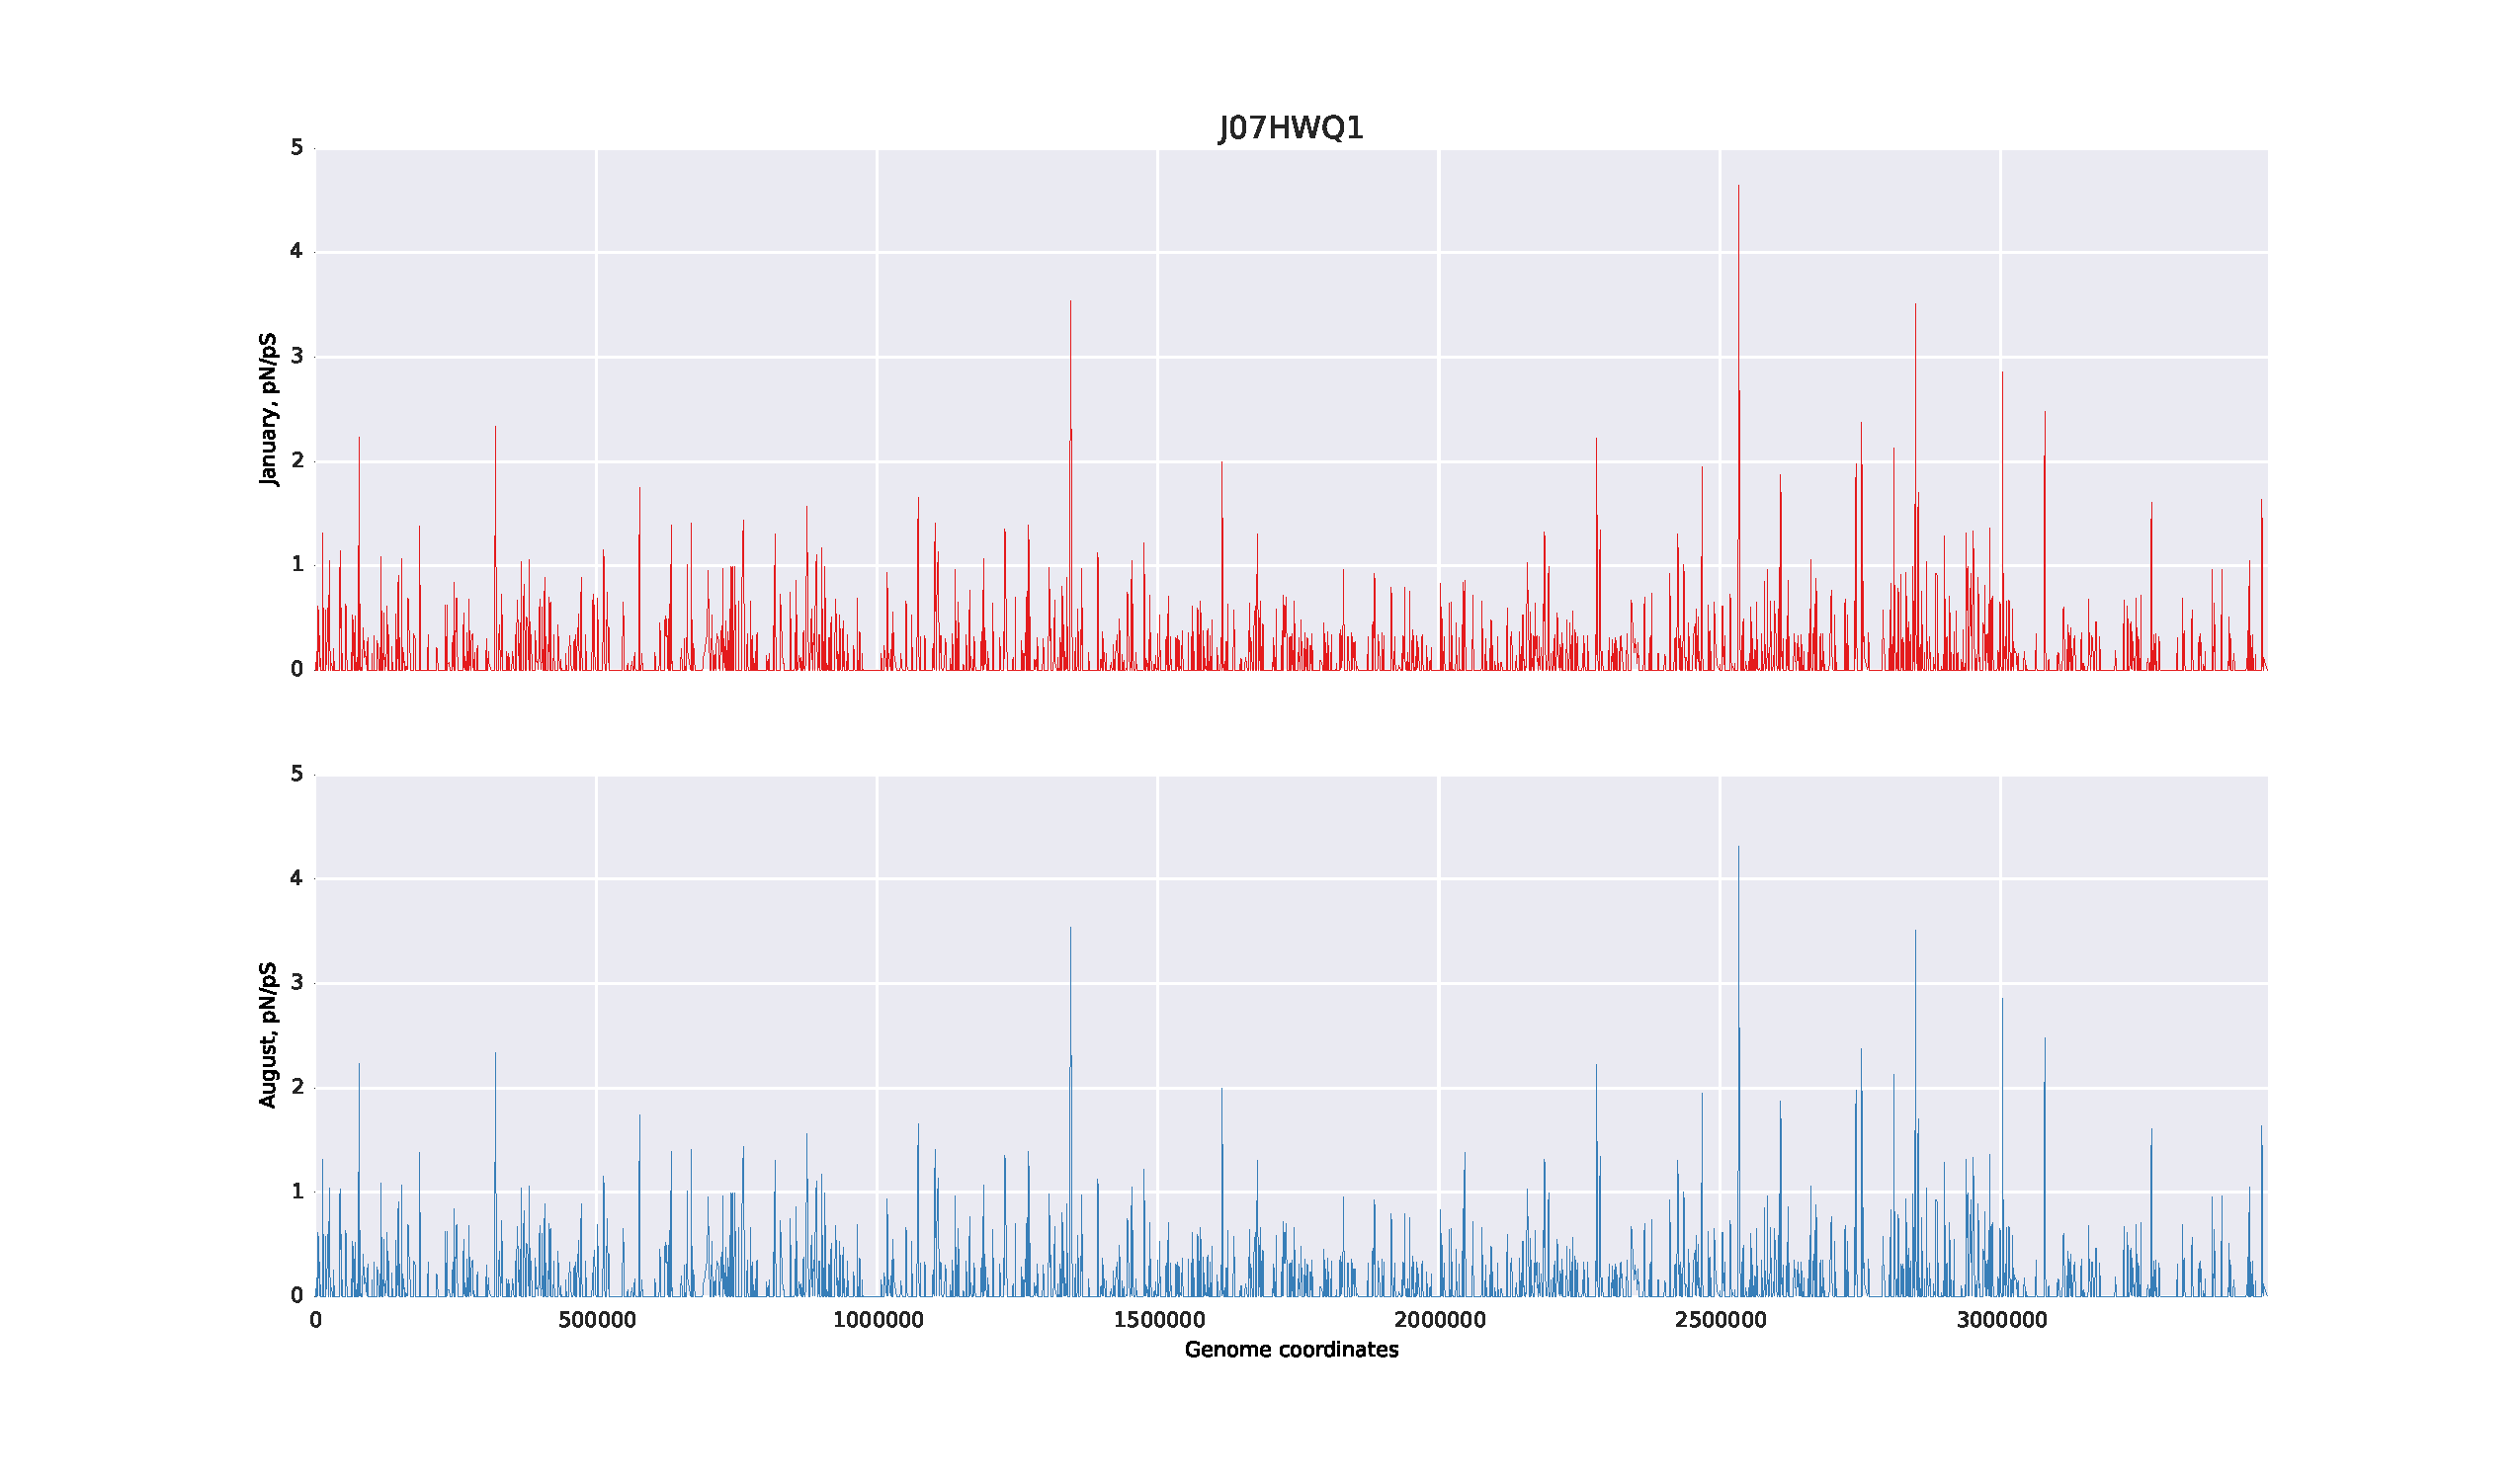
\includegraphics[width=\textwidth,height=\textheight,keepaspectratio]{Chapter5/Figures/pn_ps_plots/J07HWQ1_pNpS_density.pdf}
  \caption{pN/pS values for each gene in the J07HWQ1 genome. Top panel shows the values using the reads from the January samples. Bottom panel shows the values using the reads from the August sample.}
  \label{example_J07HWQ1_pNpS}
\end{figure}

\begin{figure}[p]
  \centering
  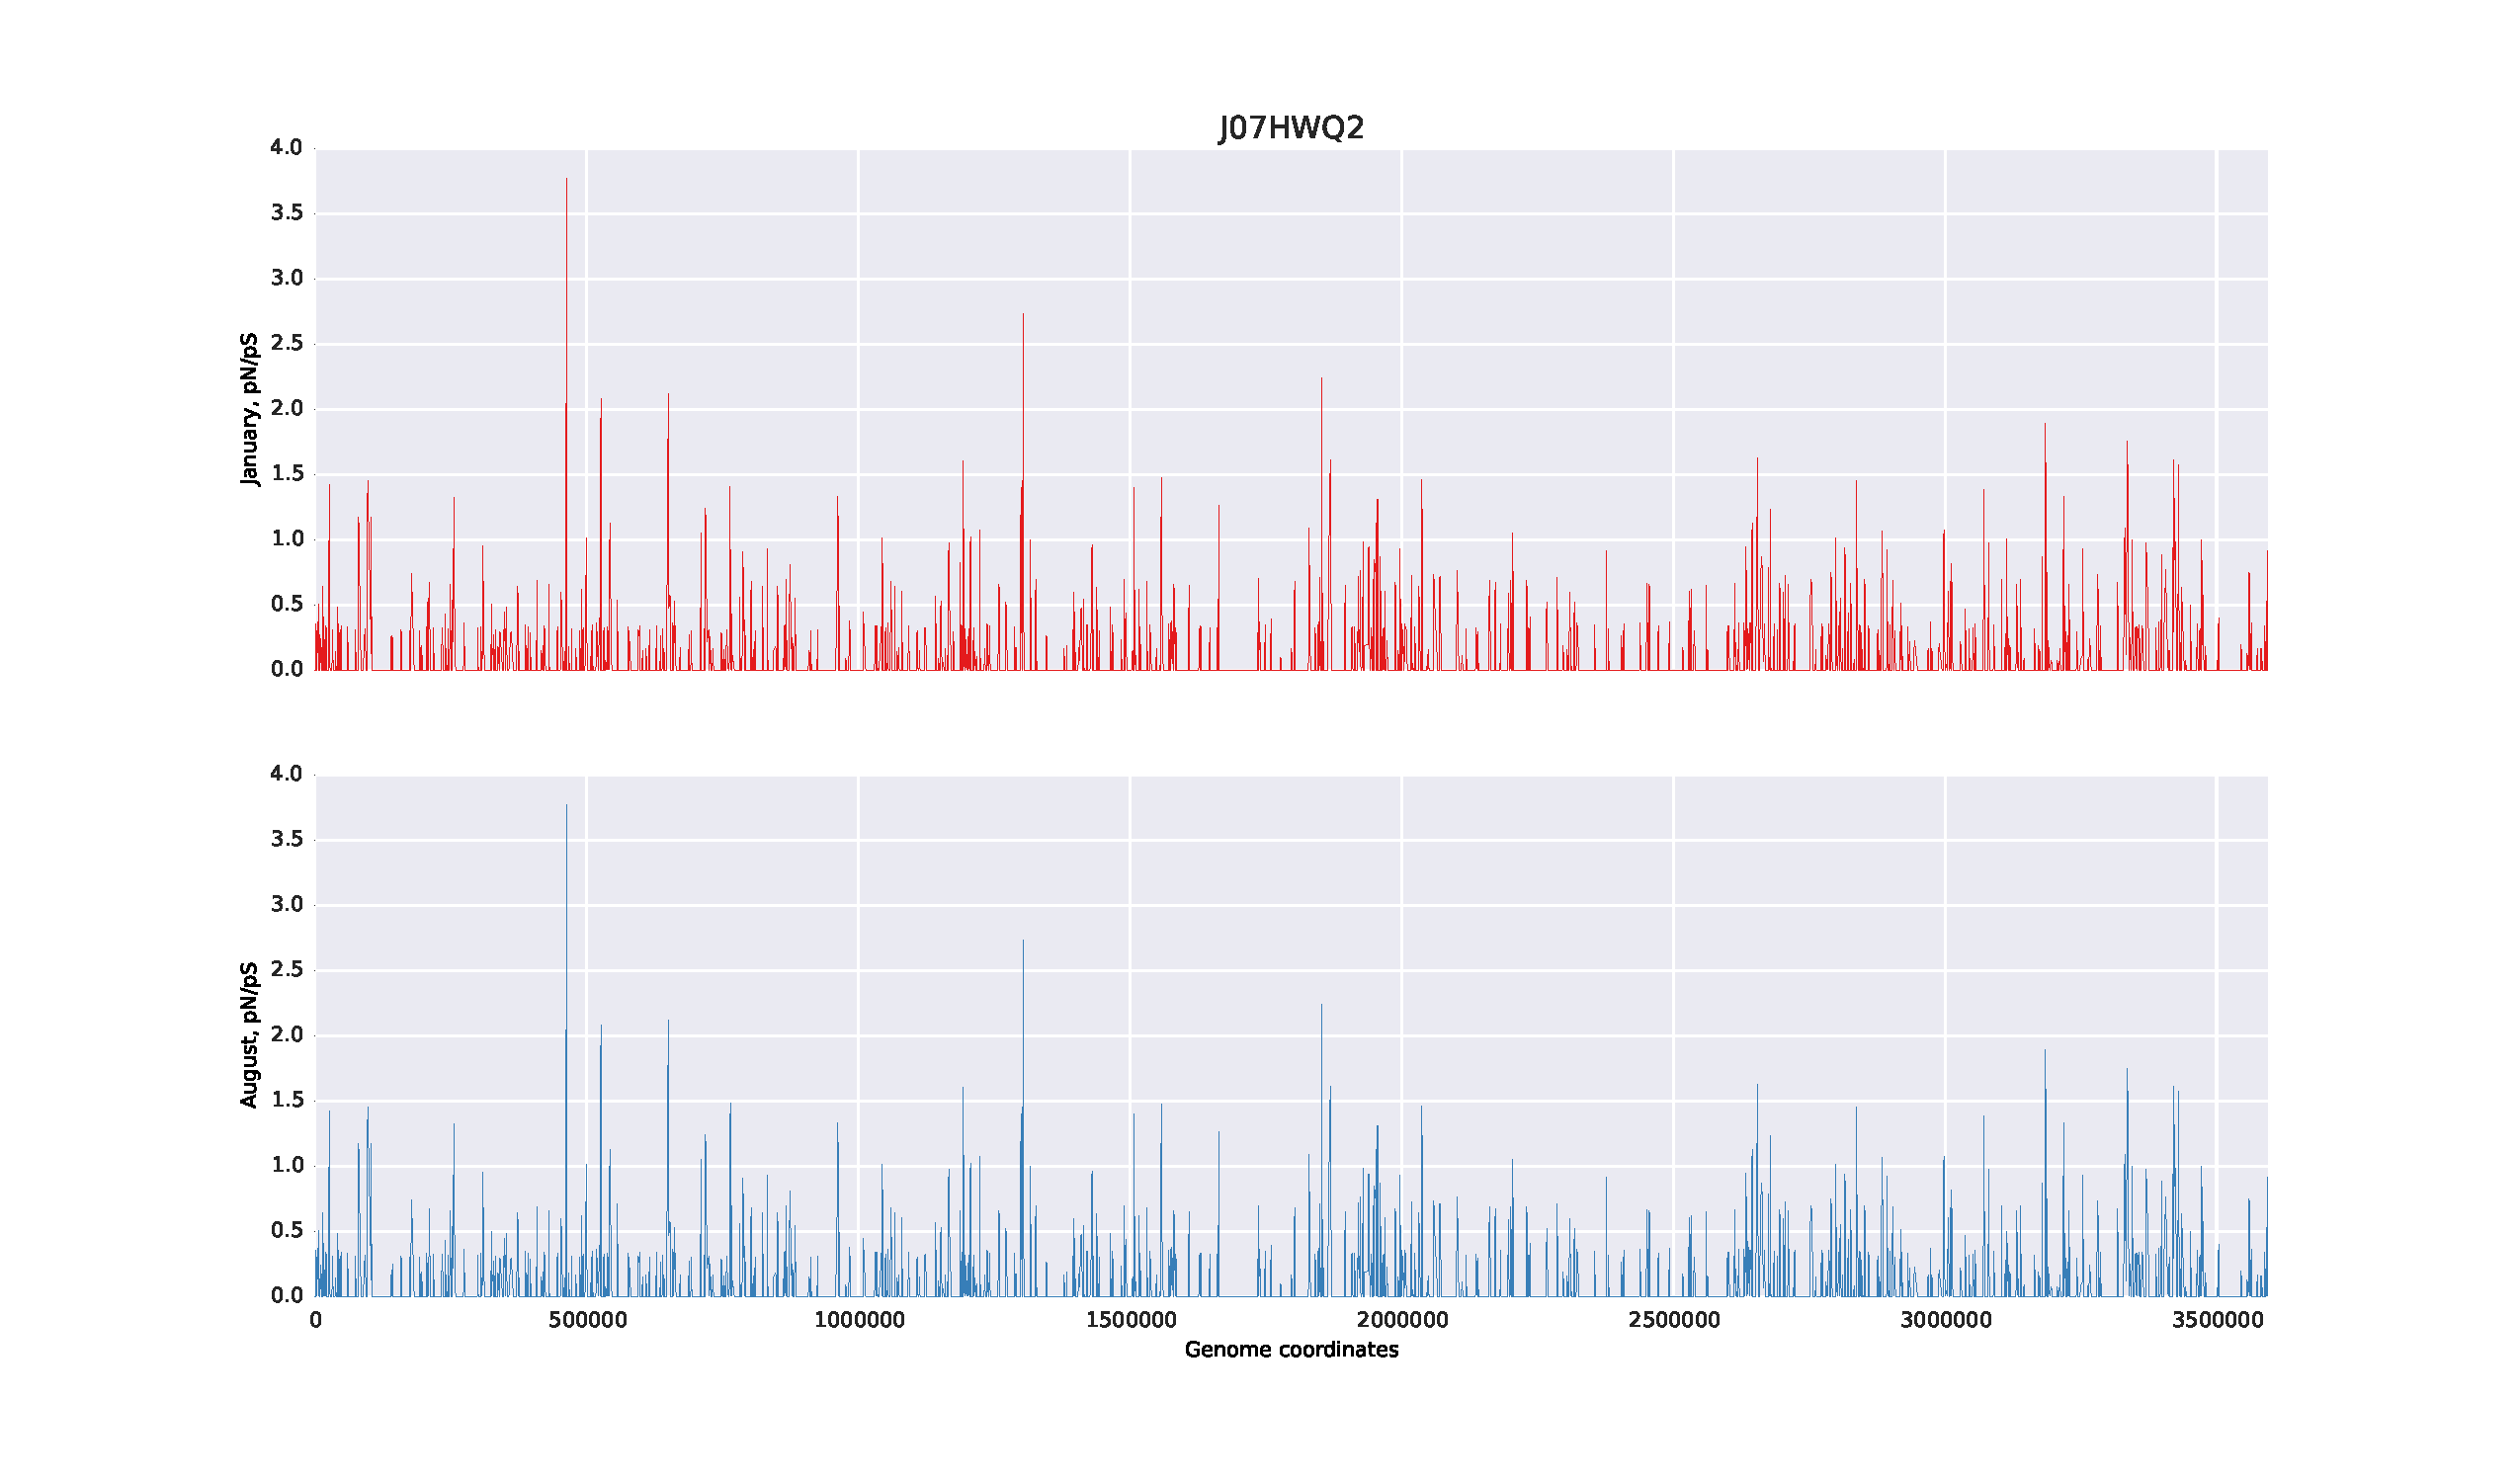
\includegraphics[width=\textwidth,height=\textheight,keepaspectratio]{Chapter5/Figures/pn_ps_plots/J07HWQ2_pNpS_density.pdf}
  \caption{pN/pS values for each gene in the J07HWQ2 genome. Top panel shows the values using the reads from the January samples. Bottom panel shows the values using the reads from the August sample.}
  \label{example_J07HWQ2_pNpS}
\end{figure}


\clearpage
\section{General Discussion}

The main goal in this Chapter, was to provide a big picture analysis of the relative abundance and fine-scale genetic diversity that is present in the Lake Tyrrell microbial community. The resulting data shows that the combination of high-throughput data, with habitat-specific genomes assembled from metagenomic datasets from the same environment \cite{Narasingarao:2012kp,Podell:2013kx,Podell:2013fp}, provides an opportunity to evalute the relative abundance of the members of the microbial community, and allows the exploration of the genetic diversity that exists in the population.

As it was mentioned in the text, some of the limitations of the current approach, is the stringent parameters used in the analysis. Depending on the goal in mind, these may need to change. A clear example of this, is that during the analysis, the G22 genome usually recruited a low number of reads (its coverage was no larger than 1.2X). This also highlights the issue of isolates and their real abundance in natural microbial communities. G22 was isolated from water samples collected in August of 2007, and chosen for genome sequencing based on similarities with the A07HB70 genome \cite{Ugalde:2013hb}. Based on the results presented here, it seems that not only this is a different species (maybe even more distant) than A07HB70, but also that its abundance in the Lake Tyrrell community is low. 

Another element that needs to be taking in consideration is the viral component of the community. Recently, several assembled viral genomes from members of this community were described \cite{Emerson:2012gh,Emerson:2013ck}. Although the filtering strategy (direct water into a Sterivex) did not enriched for viruses, using these genomes will allows us to evaluate the relative abundance of the viruses within the sequence dataset, and in addition provide an overview of the fine-scale genetic diversity that could be present on these phage genomes. It is possible that the low variation between the January and August samples, that was observed in the Archaeal and Bacterial genomes, is different in viral populations, as it has been suggested in other hypersaline ecosystems \cite{RodriguezBrito:2010in}.

One of the most interesting results, is the possibility that some of the populations that are present in the January community are the same that are present in August, such as the \textit{Haloquadratum} groups, and what it changes over time is the relative abundance of the genomes. To validate these observations, a more detailed population analysis need to be performed \cite{Schloissnig:2012hx,Kryazhimskiy:2008hq,Whitaker:2006gf}.

A large percentage of the genes found to be under positive selection, were found to be hypothetical proteins, similar to what has been observed in similar studies \cite{Tai:2011jo,Hemme:2010ds}. The potential of this type of analysis, both in isolate genomes and metagenomes, is that it provides a list of candidate genes for study, with the idea that even if the candidate is an hypothetical protein, the evidence that is under selection can be used to prioritize it for further studies. Along this lines, future work will include a more detailed analysis of each of the genes, including hypothetical proteins. For example, the incorporation of structure modelling may provide some additional information, by mapping those sites that are under selection, to the three-dimensional structure of the protein. In addition, this list can constitute possible markers to look for in further metagenomic surveys of this community.

One element that was not incorporated in the current analysis is the role of horizontal gene transfer and its relationship to natural selection \cite{Wiedenbeck:2011ena}. It has been suggested that horizontally transferred genes evolve faster than duplicated genes in Bacteria \cite{Treangen:2011ca}. This suggests that some of the genes that were under positive selection, could have been acquired from other organisms.

Moving from away from the broad comparison, the attention can also be focused on individual species groups. One of the best candidate for this analysis is \textit{Haloquadratum}. Besides the two genomes assembled from the Lake Tyrrell community, there are two genome sequences from isolates that are publicly available \cite{Bolhuis:2006gm,DyallSmith:2011tu}. A pan-genome analysis of the four genomes, could help to explain some of the results for the positive selected genes. For example, it has been suggested that core genes have lower rates of selection, compared to the non-core genes (the pan-genome) \cite{Jordan:2002by,RodriguezValera:2012cg}.

Finally, most of the effort was focused on the study of the positive selected genes, as the results provide a small dataset to focus on. But, also looking at those genes under purifying selection could provide interesting information about the organisms. It should be expected that housekeeping genes will be under purifying selection, as any changes could lead to lethal mutations for the organisms \cite{Palenik:2009kx,Schloissnig:2012hx}. Also, in \textit{Eschericha coli} it has been shown that synonymous mutations alter the rates of gene expression, so is not only the role of natural selection on changing the amino acid sequence of a protein, but also on how it affects the expression of the gene.

\section{Conclusions}

The results presented in this Chapter, provide the preliminary framework of analysis to quantify and evaluate the relative abundance and fine-scale genetic variation that is present in natural microbial communities. The genes and functions identified in this Chapter to be under positive selection, can be used in the future as markers for the study of microbial communities, in particular for future work in the Lake Tyrrell ecosystem. 

The methods and results described here, represent one of the few studies where habitat-specific genomes are used to quantify the genetic diversity present in a community. This work provides the first overview of this genetic diversity, generating the necessary data that will be required for further detailed analysis. In addition, the methods developed here, can be applied to other microbial communities, and are not limited to the study of the Lake Tyrrell hypersaline community.

\section{Acknowledgments}
I would like to thank Sheila Podell for discussions on the analysis and ideas for this Chapter. Also, funding from Fulbright-Conicyt and NSF XXXX is acknowledged, and to Amazon Web Services for an education grant that allowed the use of the EC2 infrastructure.




%%%%%%%%%%%%%%%%%%%%%%%


%\todo{Modify reference SNPs section}
%\subsection{Genome information and reference SNPs}
%To generate a list of reference SNPs,  11 archaeal genomes obtained from the assembly of the metagenomic samples were analyzed. The results (Table \ref{GenomeTable}), shows the total number of SNPs identified in each of the genomes. Although the low depth of the analysis does not allow to make any assumptions about the levels of genetic heterogeneity present on each population, still can provide a valid picture that can be contrasted with the Illumina data. Figure \ref{ReferenceSNPsType}, shows a comparison of the location and type of variation found among the genomes. Most of the identified polymorphisms are synonymous, meaning that they do not produce any changes in the amino acid sequence. Comparing among the populations, most of the polymorphisms fall into coding regions, with some extreme cases such as in \textit{Nanosalina} sp. J07AB43 and \textit{Nanosalinarum} sp. J07AB56, where only 5\% and 8\%, respectively, of the polymorpshism are found in intergenic regions. This reflects the streamlined nature of these genomes, and their reduced intergenic space \cite{Narasingarao:2012kp}. An interesting situation occurs in the case of \textit{Nanosalina} sp. J07AB43, which has a high number of polymorphisms classified as other (mostly frameshifts), close to a 51\%. This could be either result from assembly problems, or a reflection on the true genetic variability that is present in this population, but a higher level of resolution is needed to resolve this question.
%
%By looking at the annotation of each gene, we can begin to explore the possible functional effects of the found SNPs on each microbial population (Figure \ref{COG_TotalSNPs}). The averages values for each functional classification (Cellular Processes and Signaling: 19.1\%, Information Storage and Processing: 22.6\%, Metabolism: 39.9\% and Poorly characterized: 18.4\%), shows a higher percentage of SNPs (in average) in the metabolic functions. This can easily be explained by the larger number of genes that fall in this category. Even with this in mind, J07HQX50 shows a higher percentage of SNPs associated in the Cellular Processes and Signaling category, while J07AB43 and J07AB56 (members of the \textit{Nanohaloarchaea}) have a higher number of polymorphic sites in genes in the Information Storage and Processing and the Metabolic categories.
%
%Another important way to characterize the effects of the SNPs on each genomes is to look at the non-synonymous substitutions that are occurring across the genome, because the effect of this polymorphisms is to modify the resulting amino acid in the protein. The averages for each functional classification (Cellular Processes and Signaling: 18.1\%, Information Storage and Processing: 23.1\%, Metabolism: 38.5\% and Poorly characterized: 20.13\%), shows very similar values to the total count of SNPs (\ref{COG_NonSynSNPs}). Although the number of total and non-synonymous SNPs found in this part of the analysis is low to draw any conclusions about the effect on the overall microbial population, we observe that in the case of J07HR59 there are no non-synonymous polymorphisms associated with Cellular Processes and Signaling, while most fall in the Information category.
%
%To look more in detail at the effect of these non-synonymous SNPs, we can look more in detail at the functional classifications provided by COG. In the Cellular Processes and Signaling group, we can observe differences for the microbial populations (Figure \ref{ReferenceSNPs_NS_CellularProc}), which could be related to the low coverage observed for this reference SNPs, in particular in the case of J07HQX50, which has most of its SNPs associated with signal transduction mechanisms. Overall, the classification of these non-synonymous SNPs, shows that the majority falls in categories such as cell wall/membrane/envelope biogenesis, post-translational modifications and signal transduction mechanisms. These are functions that are related to the interaction of the organisms with the environments, such as phage infection and resistance mechanisms (REF), transporters (REF) and overall functions where it could be expected that changes in the amino acid sequences could be beneficial for the persistence of the microbial population in the environment. A similar situation can be observed in the case of the Information Storage and Processing category (Figure \ref{ReferenceSNPs_NS_Information}), where the more abundant in functions such as translation, ribosomal structure and biogenesis, and in proteins classified in the replication, recombination and repair group. Later in this chapter, we will explore the environmental adaptations of each microbial population, by using a deep-sequencing approach.
%
%In the case of functions that are part of the Metabolism group in the COG classification (Figure \ref{ReferenceSNPs_NS_Metabolism}), the trend is not as clear as in the other groups. The only two exceptions are J07HQX50 that has most of its polymorphisms associated with the inorganic ion transport and metabolism category, and J07HR59 that has most polymorphisms in the nucleotide transport and metabolism category. 
%
%Overall, this preliminary overview provides a set of expectetions on further analysis on the genetic heterogeneity of some of the microbial populaitons present in the Lake Tyrrell habitat. More important, by deconstructing the assembly of the Sanger reads, we can obtain a set of reference SNPs, which can be used for further population studies. This becomes very important consdiering that none of the organisms that were reocvered from the metagenoms is in culture, so targeting their genomes directly for SNP validation is not feasible, and other proxies need to be used. This dataset will be used for validation of the results of the mapping and variation detection in the following sections of this chapter.
%
%%TABLES
%
%\begin{table}[!htdp]
%\caption{Genome and reference SNPs}
%\begin{center}
%\resizebox{\textwidth}{!}{%
%\begin{tabularx}{\textwidth}{lp{2cm}p{2cm}p{3cm}}
%\hline
%%\textbf{Genome} & \textbf{Scaffold (JGI ID)} & \textbf{Length} & \textbf{SNPs} & \textbf{Change rate} \\
%\textbf{Genome}  & \textbf{Length} & \textbf{SNPs} & \textbf{Change rate} \\
%
%\hline \hline
%\multirow{2}{*}{\textit{Halonotius} sp. J07HN4} & 547,037 & 963 & 568\\
%& 2,341,623 & 7,985 & 293 \\
%\hline
%
%\multirow{6}{*}{\textit{Halonotius} sp. J07HN6} & 61,036 & 603 & 101 \\
% & 89,290 & 558 & 160 \\
% & 185,112 & 1,482 & 124 \\
% & 424,200 & 2,761 & 153 \\
% & 873,166 & 6,463 & 135 \\
%& 896,196 & 5,455 & 164 \\
%\hline
%
%uncultured archaeon sp. J07HX64 & 2,982,938 & 5,468 & 545 \\
%\hline
%\multirow{3}{*}{\textit{Halobaculum} sp. J07HB67} & 110,024 & 62 & 1,744 \\
%& 254,249 & 145 & 1,753 \\
%& 2,285,274 & 2,855 & 800 \\
%\hline
%
%\multirow{2}{*}{\textit{Haloquadratum} sp. J07HQX50} & 1,543,888 & 28 & 55,138 \\
%& 1,476,021 & 131 & 11,267 \\
%\hline
%
%\multirow{4}{*}{\textit{Halorubrum} sp. J07HR59} & 72,446 & 1 & 72,466 \\
%& 49,857 & 29 & 1,719 \\
%& 184,023 & 7 & 26,289 \\
%& 1,672,266 & 255 & 6,557 \\
%\hline
%
%\textit{Haloquadratum walsbyi} J07HQW1 & 3,475,501 & 24,743 & 140 \\
%\hline
%
%\textit{Haloquadratum walsbyi} J07HQW2 & 3,594,539 & 13,897 & 258 \\
%\hline
%
%uncultured archaeon J07HX5 & 2,040,945 & 2,047 & 997 \\
%\hline
%
%\multirow{7}{*}{\textit{Nanosalina} sp. J07AB43} & 54,503 & 295 & 184 \\
%& 111,825 & 1,037 & 107 \\
%& 65,032 & 876 & 74 \\
%& 32,088 & 304 & 105 \\
%& 112,863 & 2,296 & 49 \\
%& 52,428 & 1,288 & 40 \\
%& 798,418 & 11,578 & 68 \\
%\hline
%
%\multirow{3}{*}{\textit{Nanosalinarum} sp. J07AB56} & 195,424 & 1,540 & 127 \\
%& 60,285 & 196 & 307 \\
%& 959,093 & 6,837 & 140 \\
%\hline
%
%
%\end{tabularx}
%}
%\end{center}
%\label{GenomeTable}
%\end{table}
%
%
%%FIGURES
%
%\begin{figure}[!htbp]
%	\centering
%	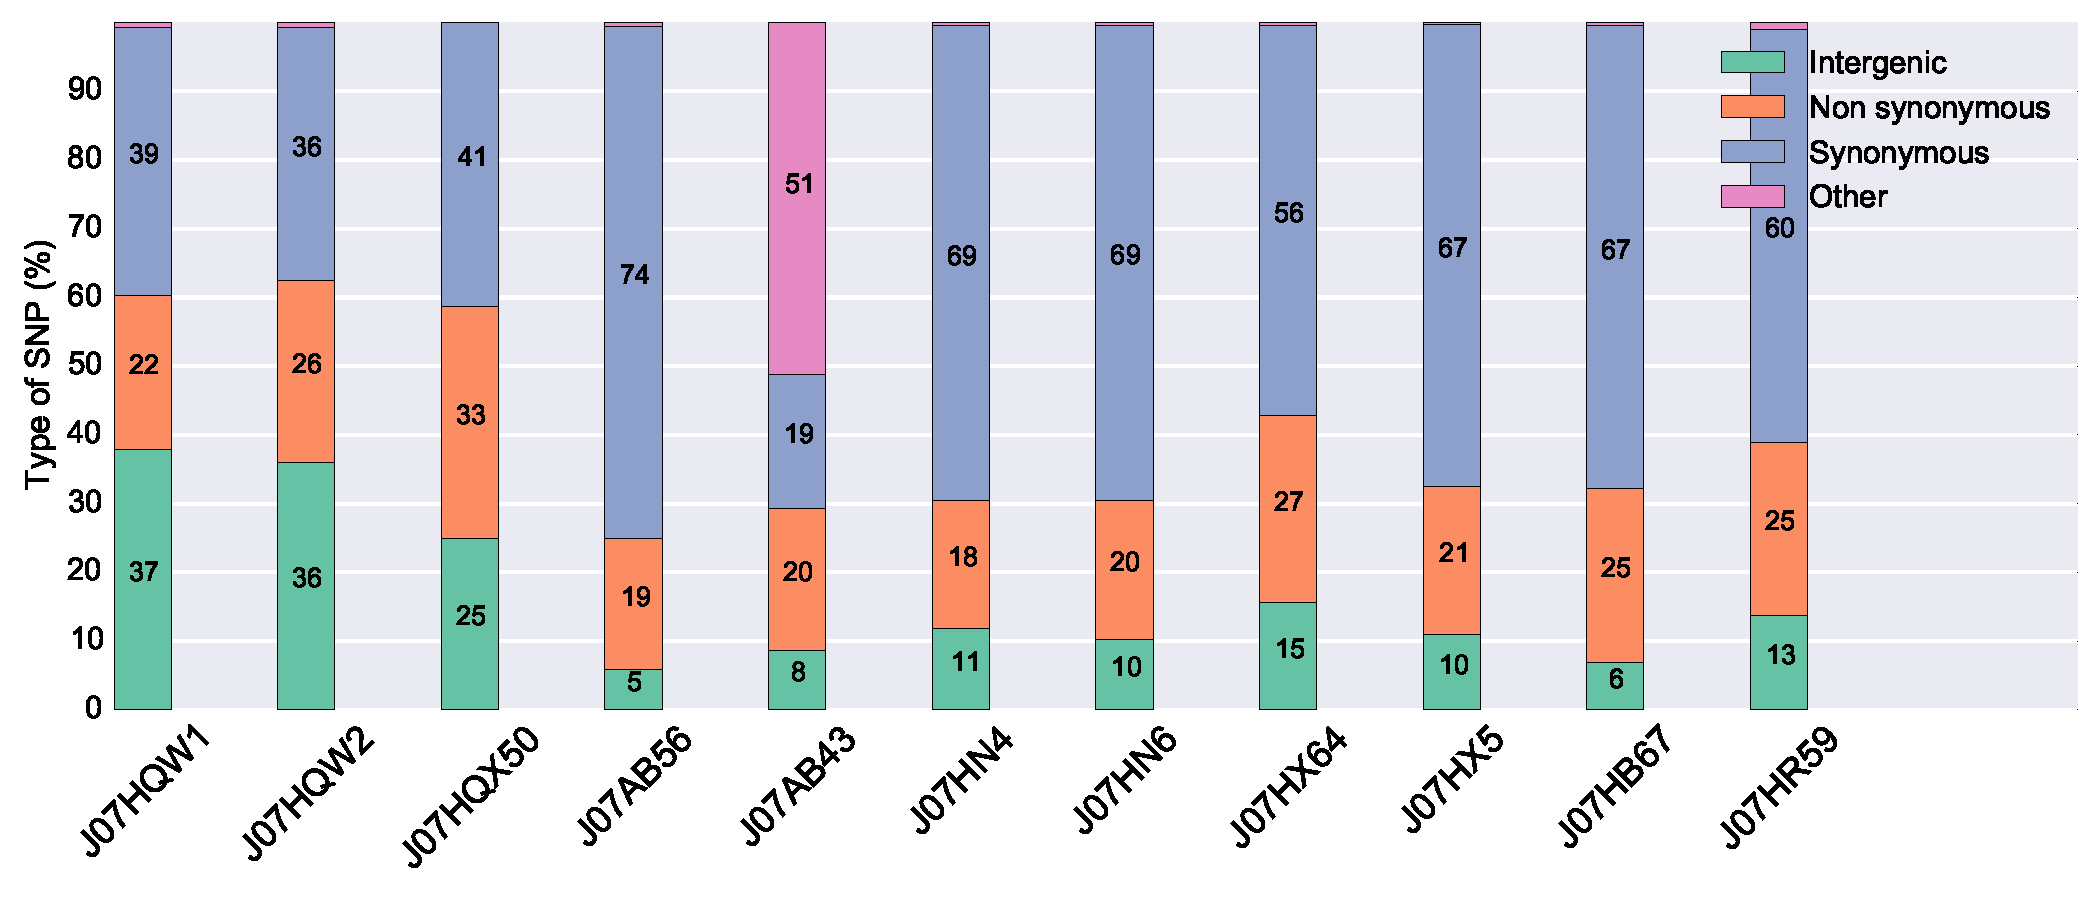
\includegraphics[width=\textwidth]{Chapter5/Figures/ReferenceSNPtypes.pdf}
%	\caption{Classification of the reference SNPs, by type.}
%	\label{ReferenceSNPsType}
%\end{figure}
%
%%FIGURE
%\begin{figure}[!htbp]
%	\centering
%	\subfloat[Total SNPs \label{COG_TotalSNPs}]{%
%		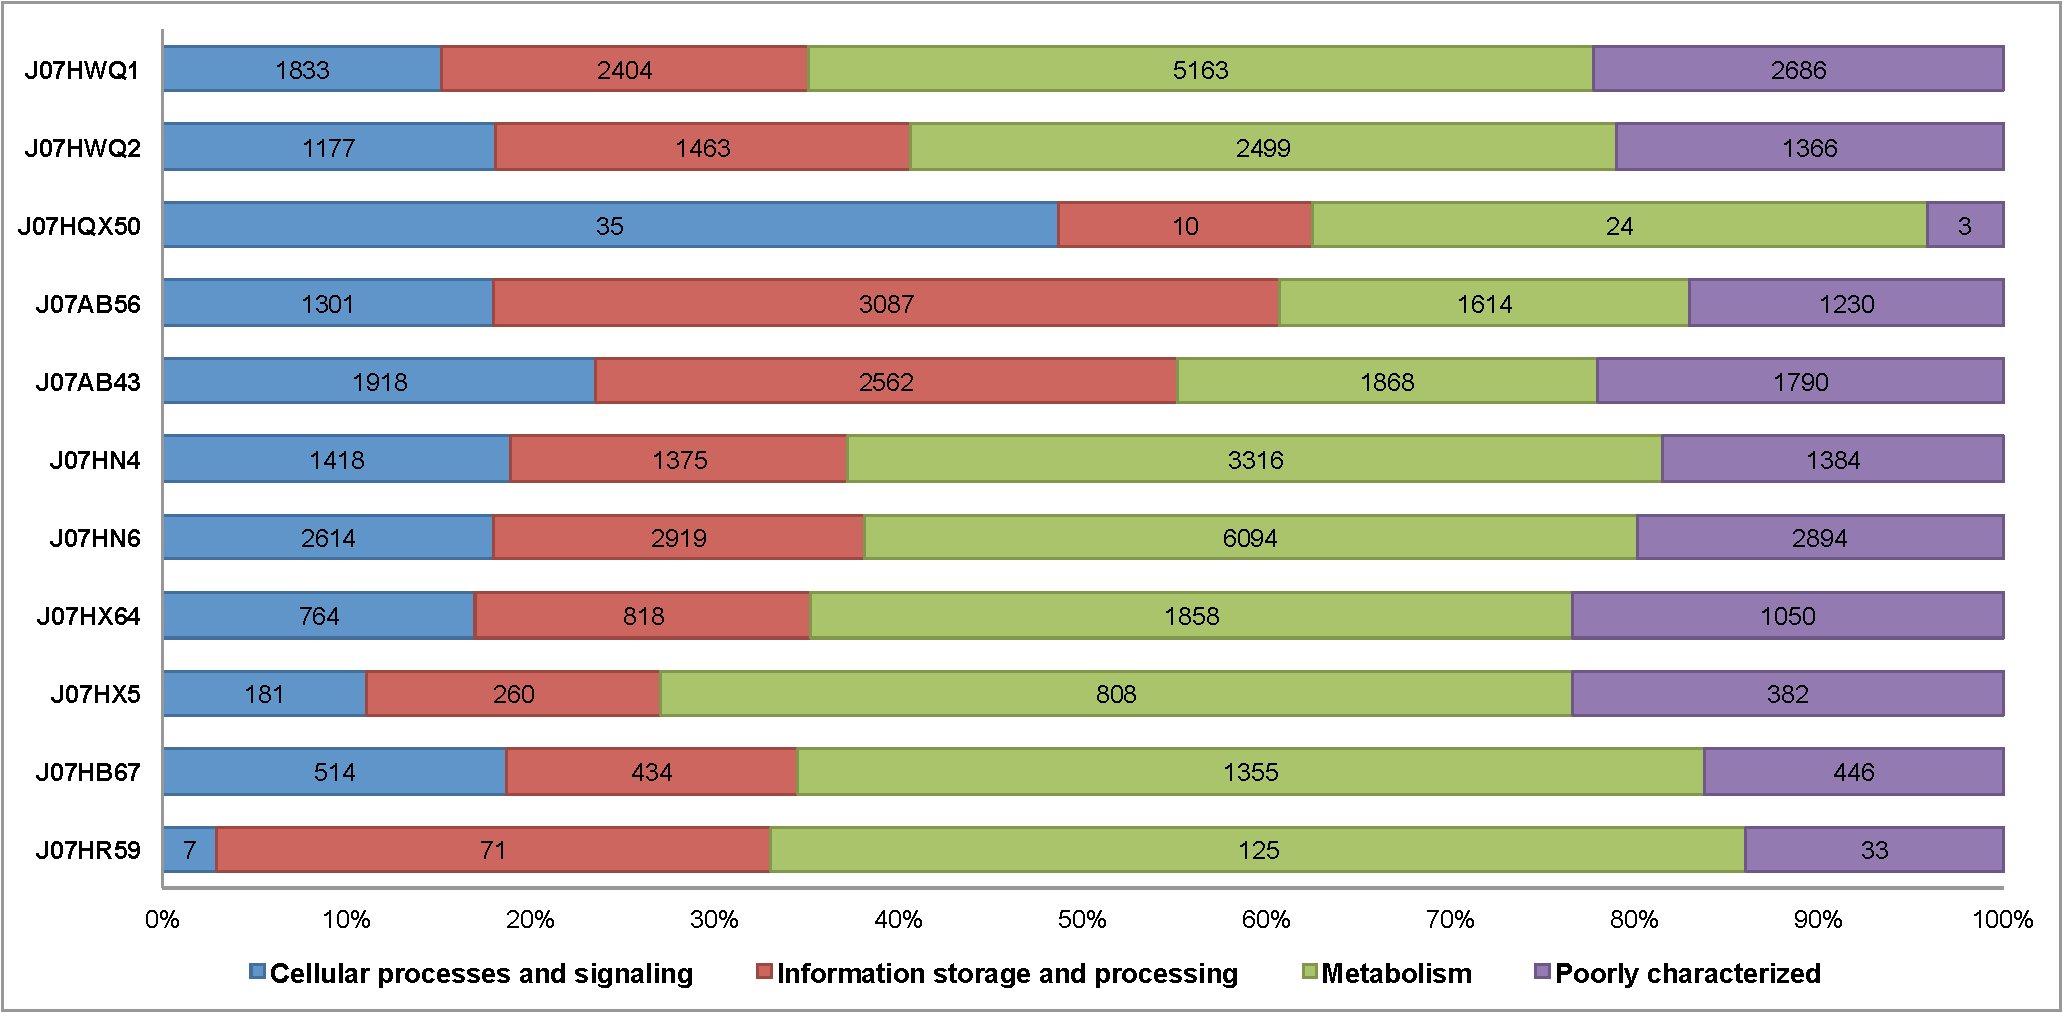
\includegraphics[width=\textwidth]{Chapter5/Figures/ReferenceSNPs_COGsTotal.pdf}
%	}
%	\hfill
%	\subfloat[Non-synonymous SNPs\label{COG_NonSynSNPs}]{%
%		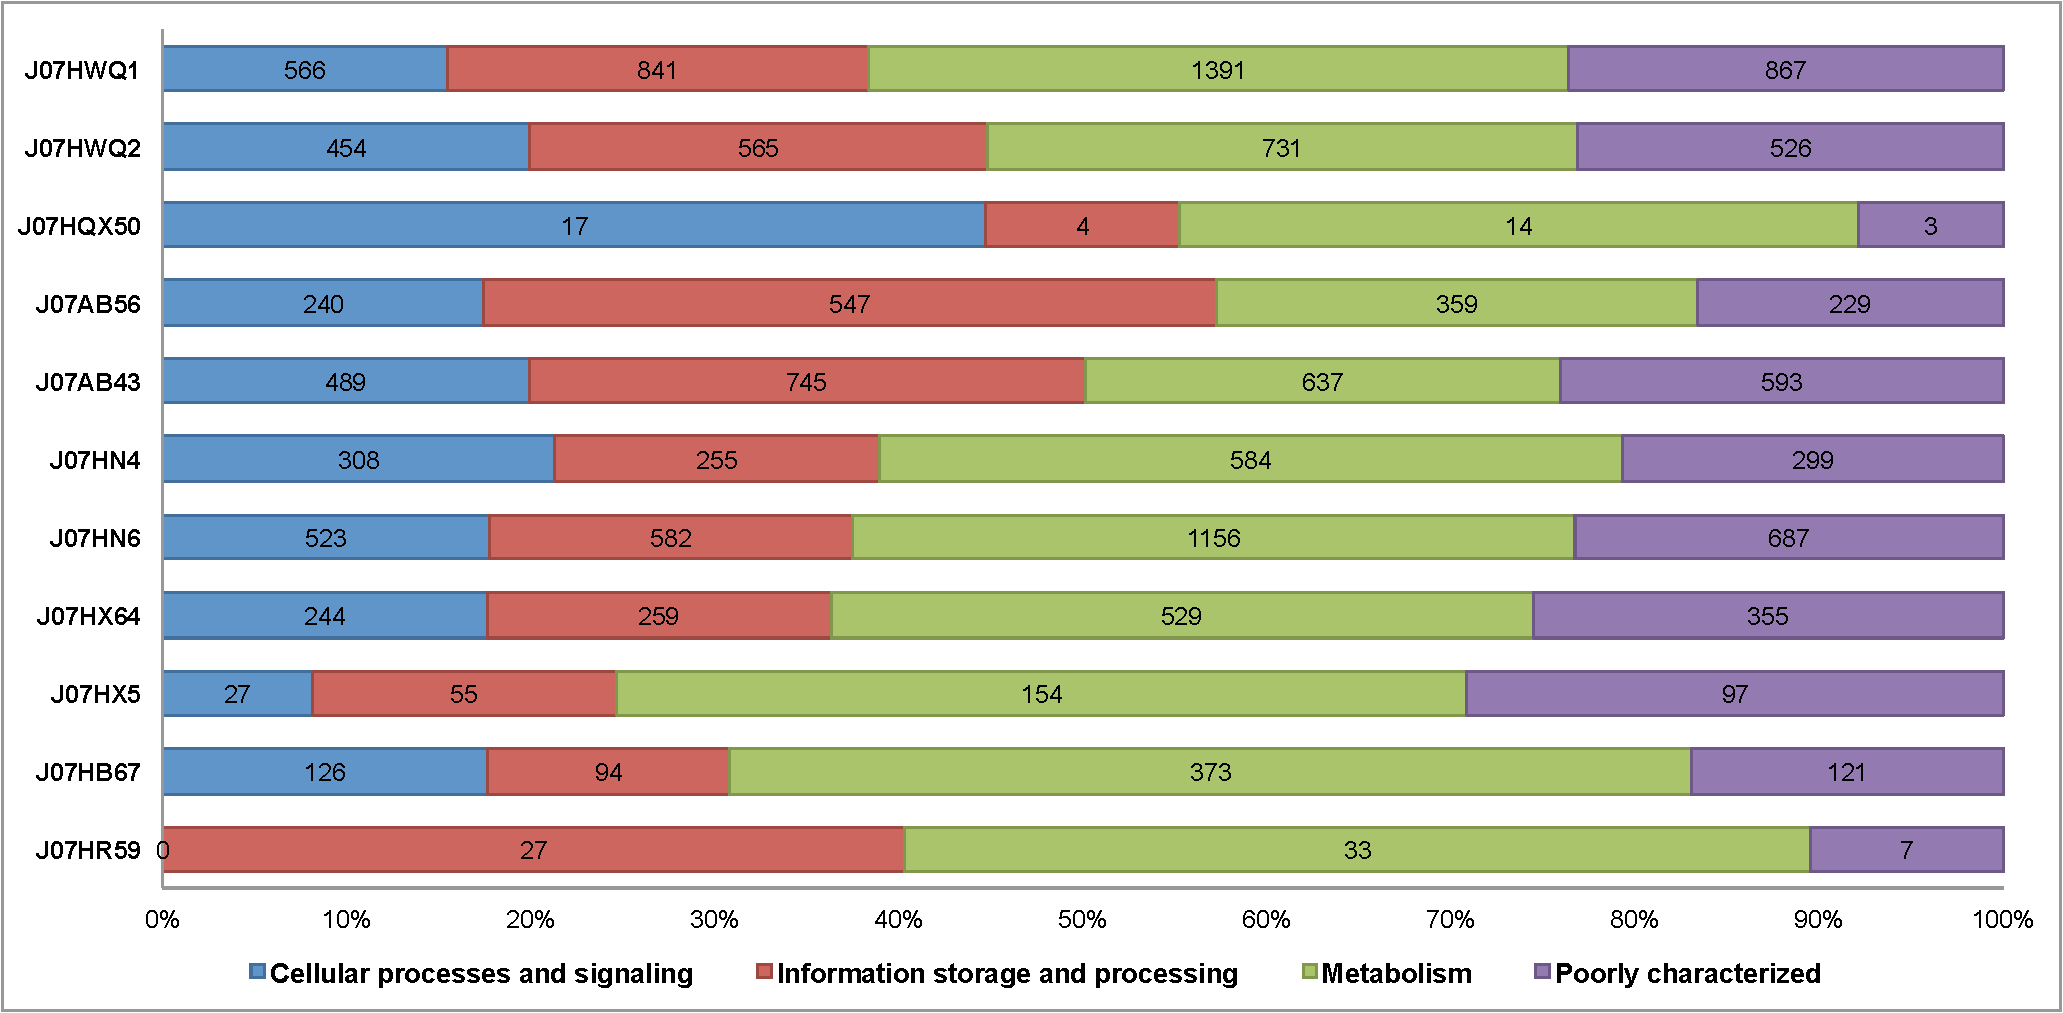
\includegraphics[width=\textwidth]{Chapter5/Figures/ReferenceSNPs_COGs_NS.pdf}
%	}		
%	\caption{Comparison between the total number and the non-synonymous SNPs found in each genome, associated to functional categories from the COG classification }
%	\label{ReferenceSNPs_COGsSummary}
%\end{figure}
%
%%FIGURE
%
%\begin{figure}[!htbp]
%	\centering
%	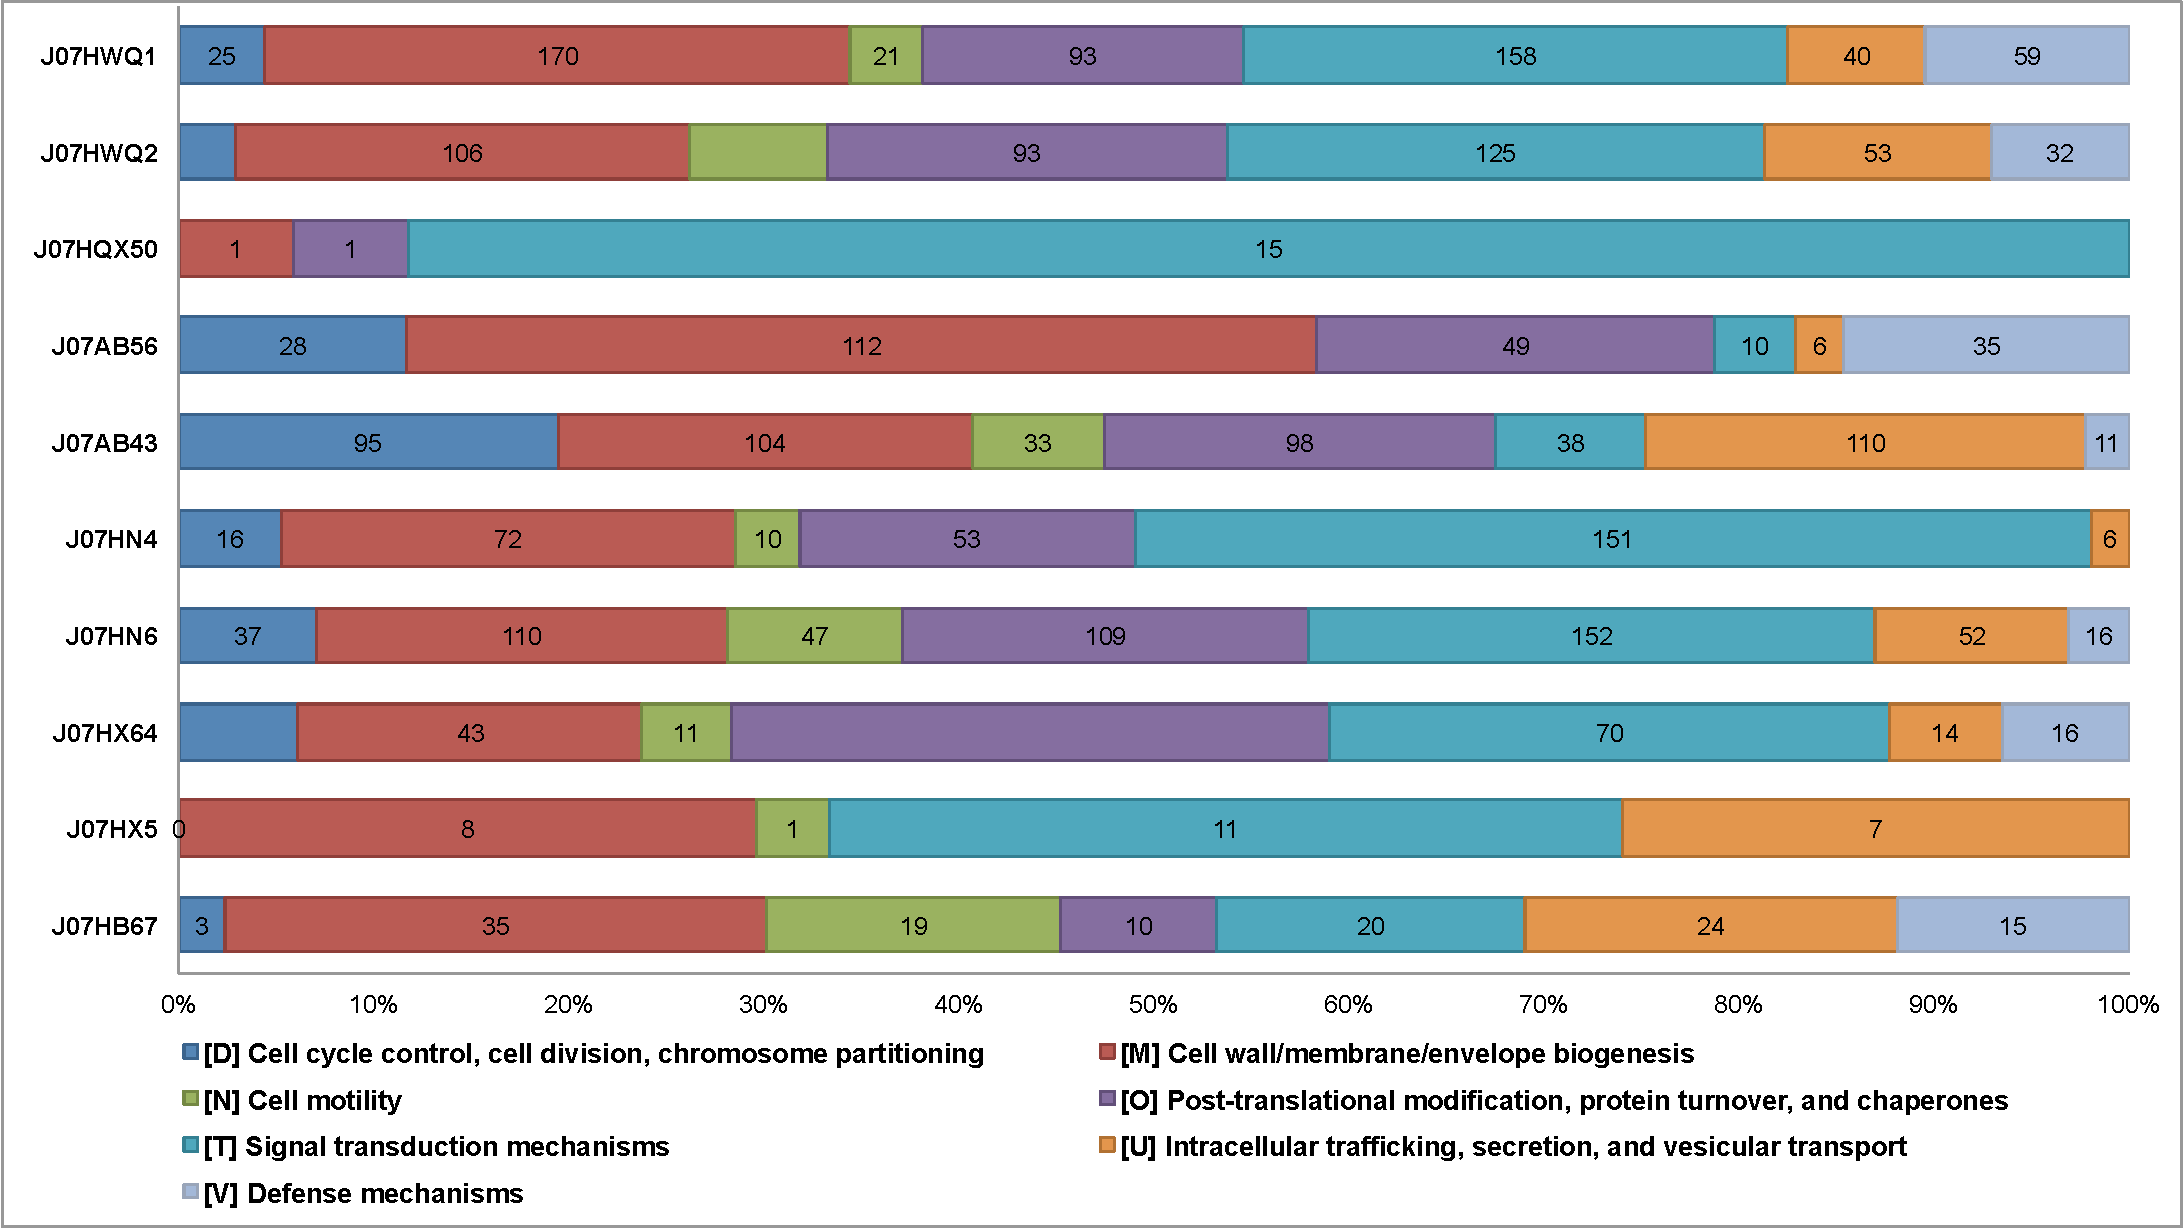
\includegraphics[width=\textwidth]{Chapter5/Figures/ReferenceSNPs_NonSyn_CellularProc.pdf}
%	\caption{Count of non-synonymous SNPs found in COGs categories from the Cellular Processes and Signaling group}
%	\label{ReferenceSNPs_NS_CellularProc}
%\end{figure}
%
%\begin{figure}[!htbp]
%	\centering
%	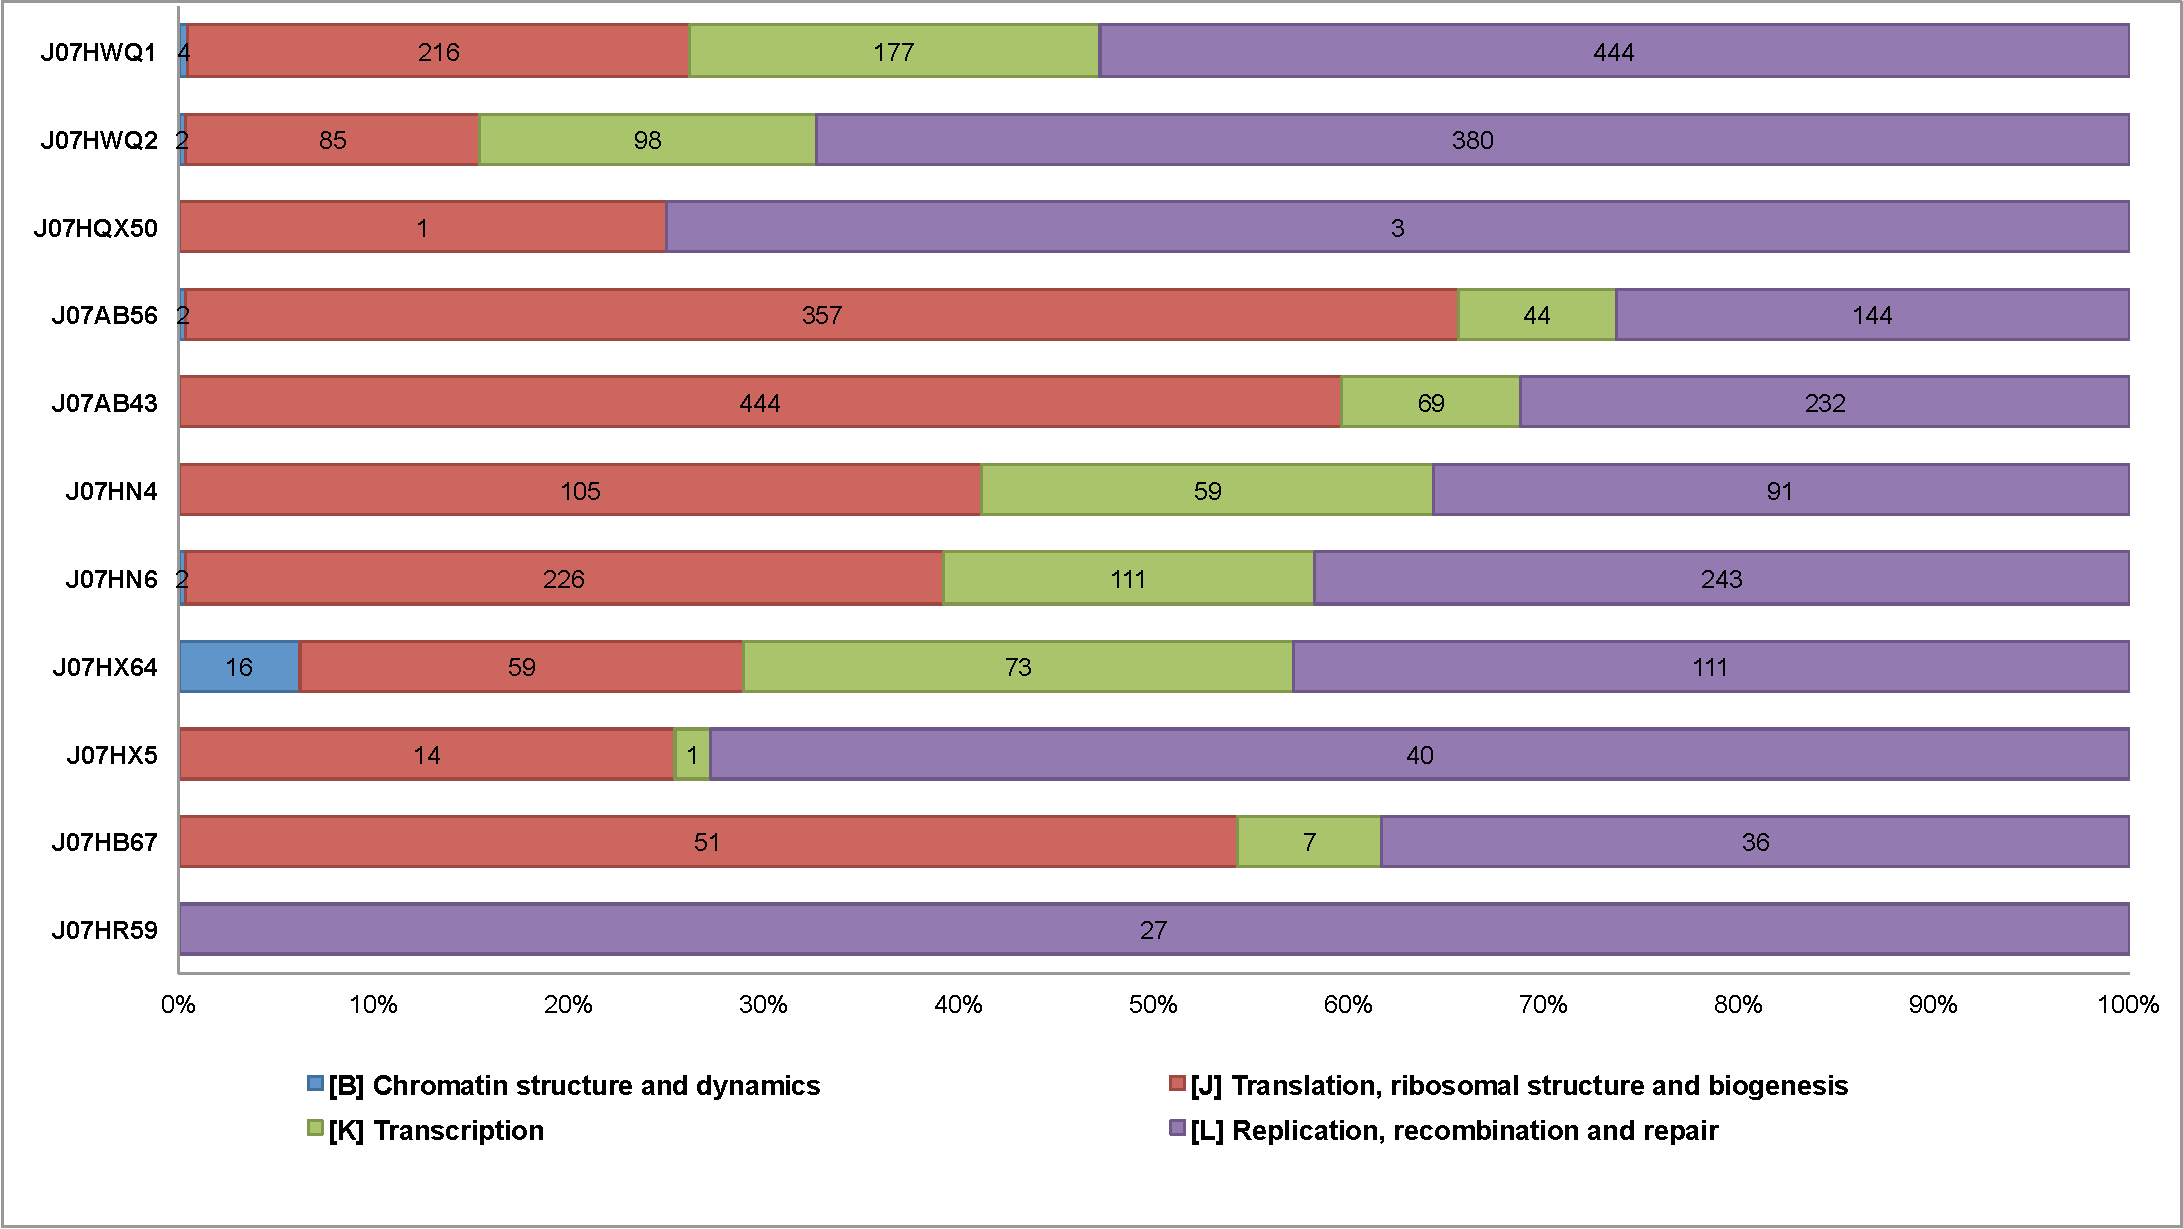
\includegraphics[width=\textwidth]{Chapter5/Figures/ReferenceSNPs_NonSyn_Information.pdf}
%	\caption{Count of non-synonymous SNPs found in COGs categories from the Information Storage and Processing group}
%	\label{ReferenceSNPs_NS_Information}
%\end{figure}
%
%\begin{figure}[!htbp]
%	\centering
%	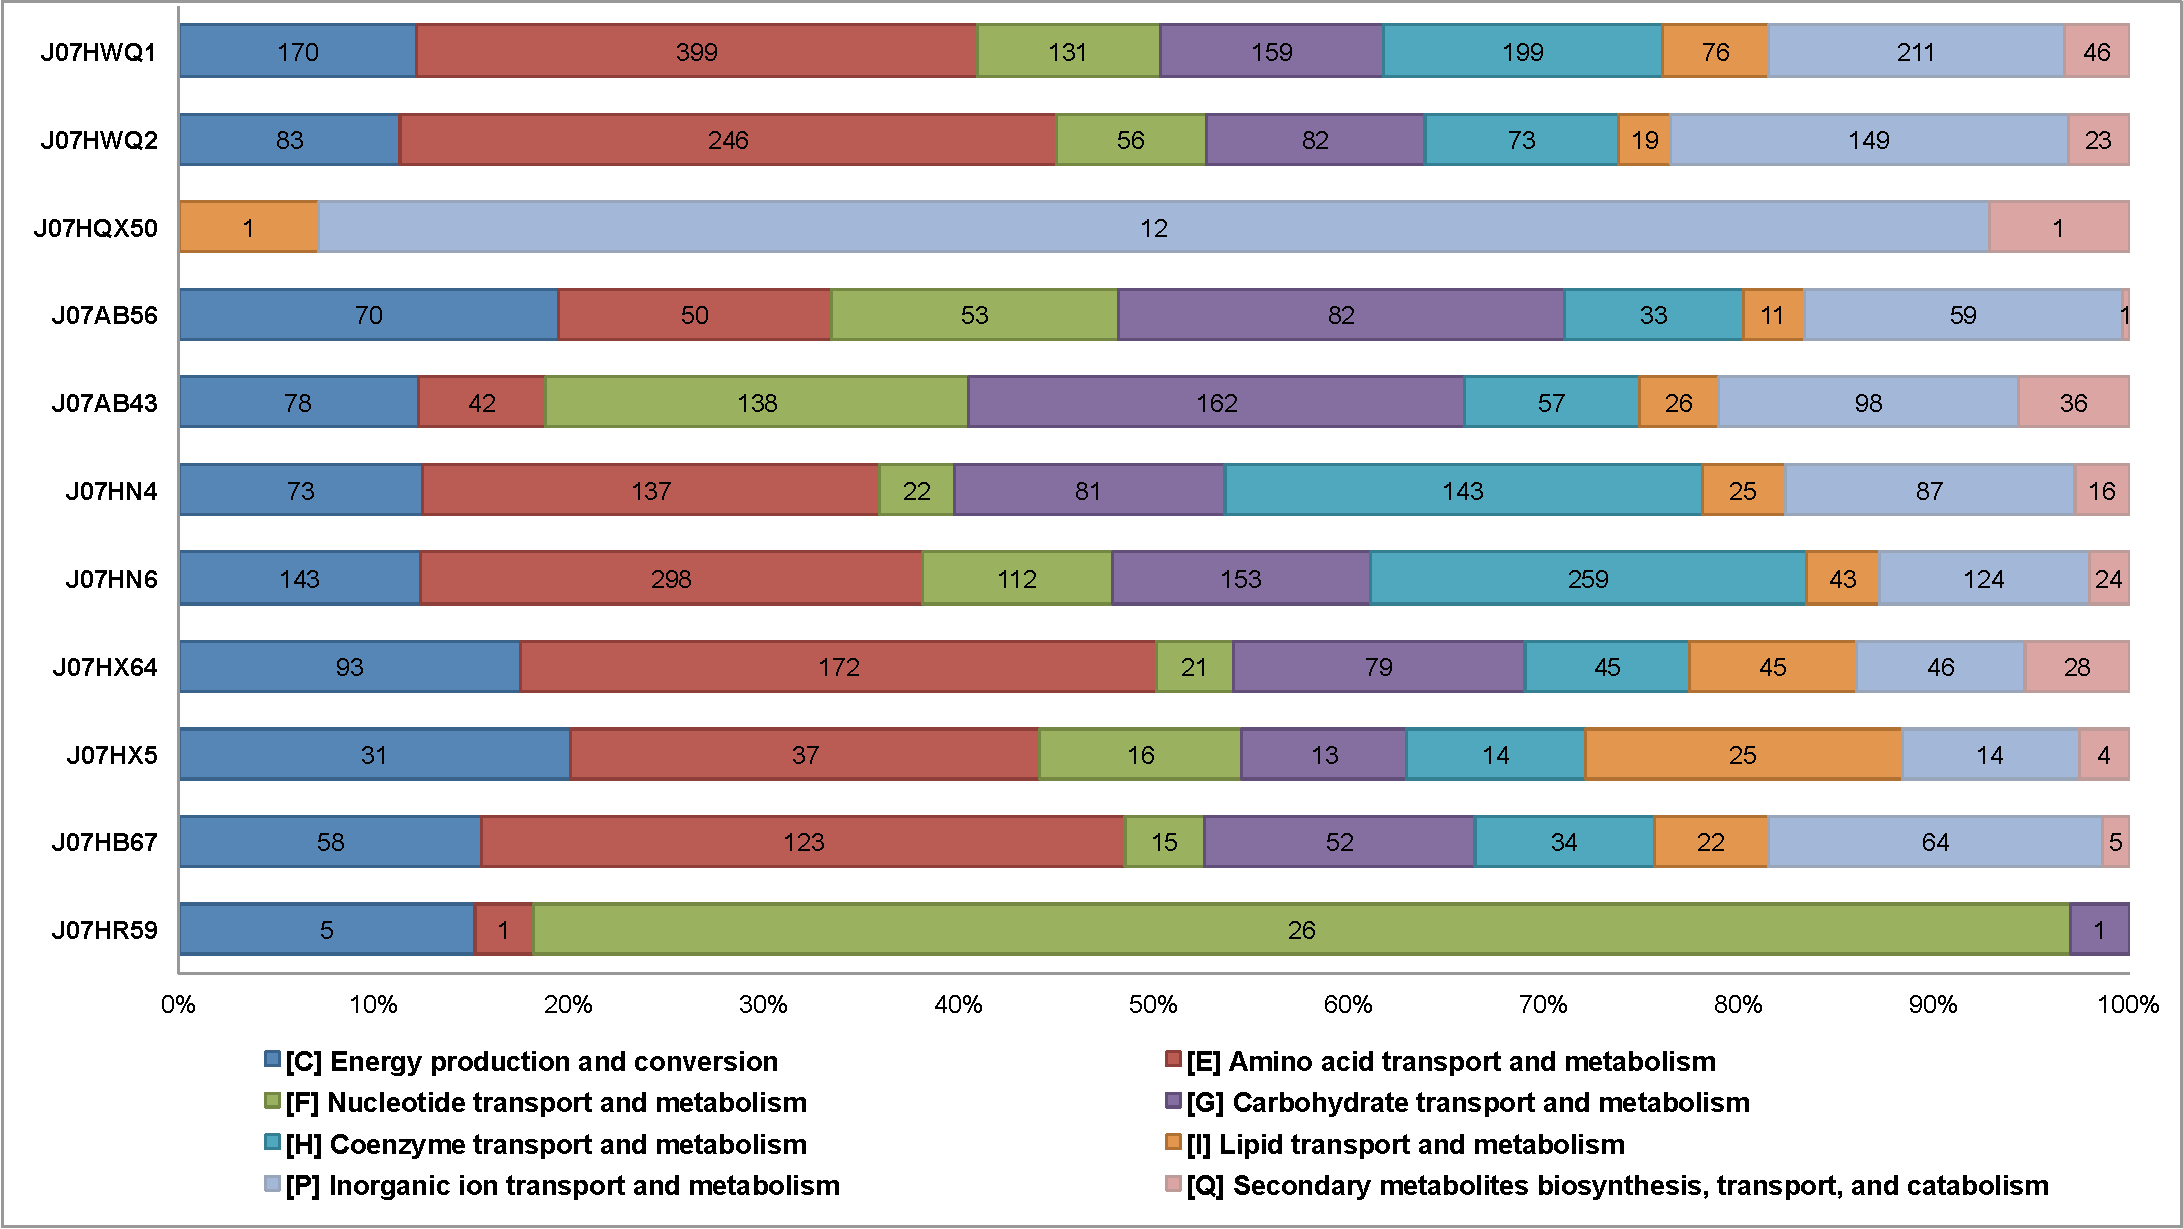
\includegraphics[width=\textwidth]{Chapter5/Figures/ReferenceSNPs_NonSyn_Metabolism.pdf}
%	\caption{Count of non-synonymous SNPs found in COGs categories from the Metabolism group}
%	\label{ReferenceSNPs_NS_Metabolism}
%\end{figure}
%
%
%

%\subsection{Selection analysis of the reference SNPs}
%- Genes found under positive selection
%- Functional differences of the genes under positive selection
%- Categories, etc

%
%
%Comparison between assembly and read mapping
%
%The comparison between the number of reads used in the assembly of the archaeal populations, versus mapping the reads back to these genomes, indicates that only a low percentage of the reads were not recovered by mapping (XX\%) (Figure X). In addition, mapping of the reads allows the recovery of reads that were not incorporated into the assemblies.
%
%Even when the number the depth of coverage is increase when the reads are mapped back to the reference genomes (Table X), the overall distribution of depths along the genome shows a similar trend (Figure X), indicating that even with that more reads are recruited (increasing the depth of coverage and posiblly the number of SNPS presents compared to an assembly-based analysis), we are not overrepreseting areas of the genome.
%
%We observed differences when looking at the coverage of individual genes, where a small percentage in each genome (XX, Table X) showed less coverage than expected. Neverhelss, this is only a small fraction of the total number of genes present (Figure X).
%
%Look at the gene with transport, secretory or motilify functions in detail. Look a the dN/dS ratiosn in a sliding window (201 bp?)
%
%For hypothetica proteins, look at SCOP classification
%


%
%\begin{figure}[htbp]
%	\centering
%	*
%	\caption{Analysis pipeline workflow}
%	\label{WorkflowAnalysisSNPs}
%\end{figure}
%
%
%\begin{figure}[htbp]
%	\centering
%	*
%	\caption{Mapped reads per genome}
%	\label{ReadMappingGenomes}
%\end{figure}
%
%\begin{figure}[htbp]
%	\centering
%	*
%	\caption{Depth of coverage for each genome}
%	\label{DepthCoverageGenomes}
%\end{figure}
%
%\begin{figure}[htbp]
%	\centering
%	*
%	\caption{SNPs in COGs}
%	\label{COGsSNPs}
%\end{figure}
%
%\begin{figure}[htbp]
%	\centering
%	*
%	\caption{Transition transversion rates}
%	\label{TTrates}
%\end{figure}
%
%\begin{figure}[htbp]
%	\centering
%	*
%	\caption{Network diagram SNPs}
%	\label{NetworkSNPs}
%\end{figure}
%
%\begin{figure}[htbp]
%	\centering
%	*
%	\caption{Map of SNPs in contigs}
%	\label{SNPsContigMap}
%\end{figure}
%
%\begin{figure}[htbp]
%	\centering
%	*
%	\caption{SNP rarefaction curve per population}
%	\label{SNPsRarefaction}
%\end{figure}
%
%\begin{figure}[htbp]
%	\centering
%	*
%	\caption{Calculation of pN/pS ratios}
%	\label{pNpS_diagram}
%\end{figure}
%
%\begin{figure}[htbp]
%	\centering
%	*
%	\caption{Histogram of dN/dS ratios}
%	\label{pNpS_hist}
%\end{figure}


%Figure SNPs in genes
%\begin{figure}[h]
%\centering
%\subfloat[January (both dates combined)]{
%    \label{Jan_SNP_boxplot}
%    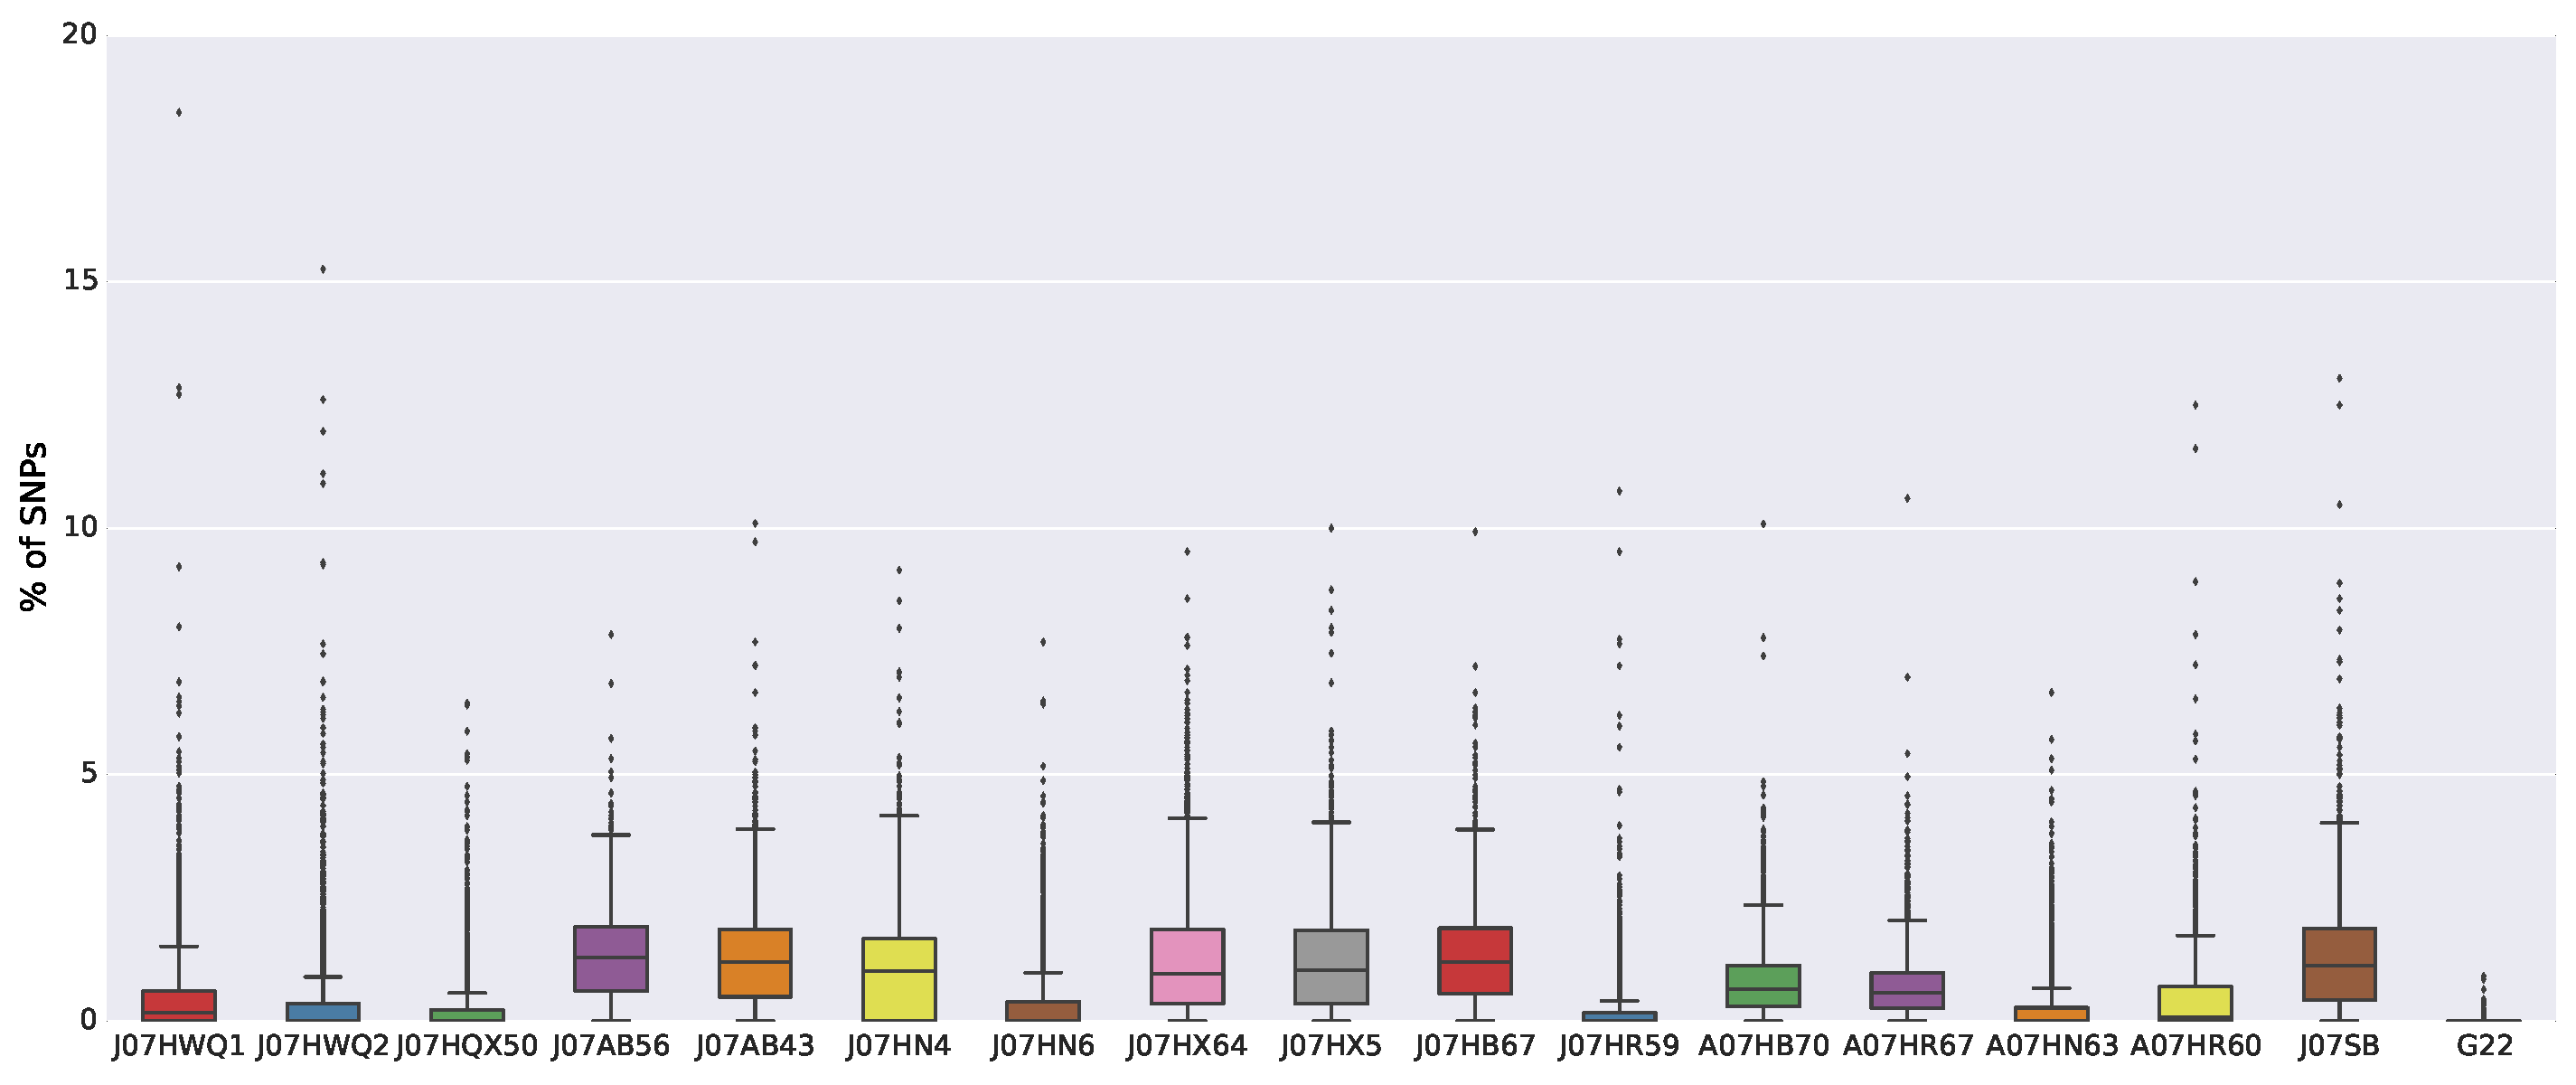
\includegraphics[width=\textwidth]{Chapter5/Figures/Jan_SNP_freq_boxplot.pdf}
%    }
%    \hfill
%\subfloat[August (both dates combined)]{
%    \label{Aug_SNP_boxplot}
%    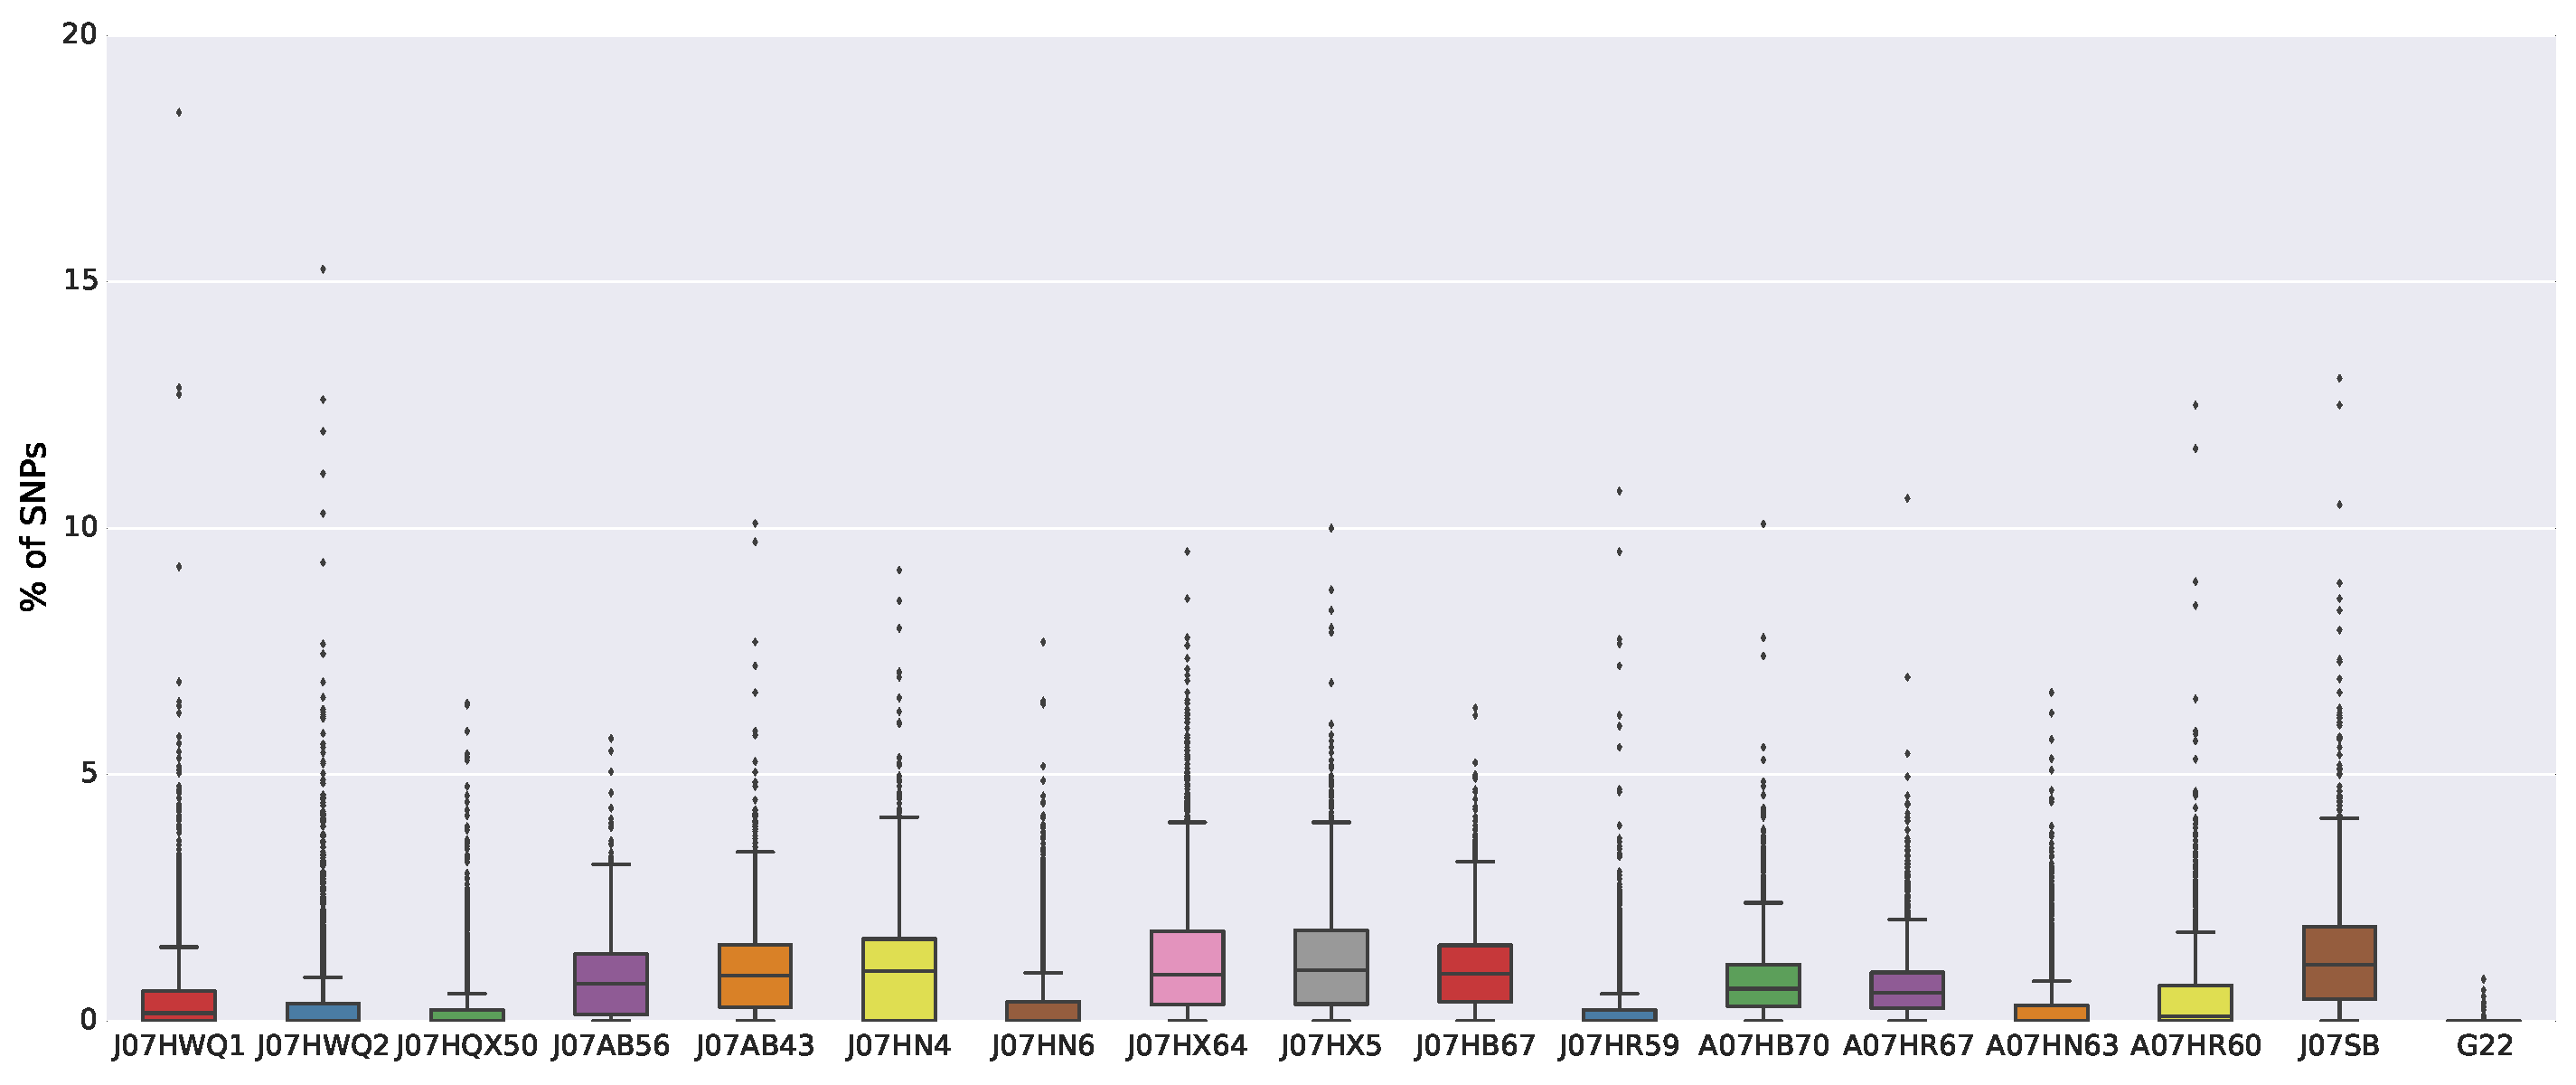
\includegraphics[width=\textwidth]{Chapter5/Figures/Aug_SNP_freq_boxplot.pdf}
%    }
%    \caption{Distribution of genes based on the percentage of SNPs present in them, in the January and August combined libraries.}
%    \label{SNPs_Boxplot}
%\end{figure}


%\bibliographystyle{abbrv}
%\bibliography{CompleteLibrary}